%
%
% UCSD Doctoral Dissertation Template
% -----------------------------------
% https://github.com/ucsd-thesis/ucsd-thesis
%
%
% ----------------------------------------------------------------------
% WARNING: 
%
%   This template has not endorced by OGS or any other official entity.
%   The official formatting guide can be obtained from OGS.
%   It can be found on the web here:
%   http://grad.ucsd.edu/_files/academic-affairs/Dissertations_Theses_Formatting_Manual.pdf
%
%   No guaranty is made that this LaTeX class conforms to the official UCSD guidelines.
%   Make sure that you check the final document against the Formatting Manual.
%  
%   That being said, this class has been routinely used for successful 
%   publication of doctoral theses.  
%
%   The ucsd.cls class files are only valid for doctoral dissertations.
%
%
% ----------------------------------------------------------------------
% GETTING STARTED:
%
%   Lots of information can be found on the project wiki:
%   http://code.google.com/p/ucsd-thesis/wiki/GettingStarted
%
%
%   To make a pdf from this template use the command:
%     pdflatex template
%
%
%   To get started please read the comments in this template file 
%   and make changes as appropriate.
%
%   If you successfully submit a thesis with this package please let us
%   know.
%
%
% ----------------------------------------------------------------------
% KNOWN ISSUES:
%
%   Currently only the 12pt size conforms to the UCSD requirements.
%   The 10pt and 11pt options make the footnote fonts too small.
%
%
% ----------------------------------------------------------------------
% HELP/CONTACT:
%
%   If you need help try the ucsd-thesis google group:
%   http://groups.google.com/group/ucsd-thesis
%
%
% ----------------------------------------------------------------------
% BUGS:
%
%   Please report all bugs at:
%   https://github.com/ucsd-thesis/ucsd-thesis/issues
%
%
% ----------------------------------------------------------------------
% More control of the formatting of your thesis can be achieved through
% modifications of the included LaTeX class files:
%
%   * ucsd.cls    -- Class file
%   * uct10.clo   -- Configuration files for font sizes 10pt, 11pt, 12pt
%     uct11.clo                            
%     uct12.clo
%
% ----------------------------------------------------------------------



% Setup the documentclass 
% default options: 12pt, oneside, final
%
% fonts: 10pt, 11pt, 12pt -- are valid for UCSD dissertations.
% sides: oneside, twoside -- note that two-sided theses are not accepted 
%                            by OGS.
% mode: draft, final      -- draft mode switches to single spacing, 
%                            removes hyperlinks, and places a black box
%                            at every overfull hbox (check these before
%                            submission).
% chapterheads            -- Include this if you want your chapters to read:
%                              Chapter 1
%                              Title of Chapter
%
%                            instead of
%                              1 Title of Chapter
\documentclass[12pt,chapterheads,final]{ucsd}



% Include all packages you need here.  
% Some standard options are suggested below.
%
% See the project wiki for information on how to use 
% these packages. Other useful packages are also listed there.
%
%   http://code.google.com/p/ucsd-thesis/wiki/GettingStarted

\usepackage[acronym]{glossaries}
%\usepackage[automake]{glossaries-extra}

%% AMS PACKAGES - Chances are you will want some or all 
%    of these if writing a dissertation that includes equations.
%  \usepackage{amsmath, amscd, amssymb, amsthm}

%% BONUS MATH
%  \usepackage{mathtools} 

%% MARGIN REQUIREMENTS IN TITLES - Hyphenation in a Section Title does not always respect margin settings in Latex.  To force no hyphentation, uncomment the package below.
%  \usepackage[raggedright]{titlesec} 

%% GRAPHICX - This is the standard package for 
%    including graphics for latex/pdflatex.
\usepackage{scrextend}
\usepackage{pslatex}
\usepackage{graphicx}
\graphicspath{ {./figures/} }

\usepackage[export]{adjustbox}
%\usepackage{verbatimbox}


%% CAPTION
% This overrides some of the ugliness in ucsd.cls and
% allows the text to be double-spaced while letting figures,
% tables, and footnotes to be single-spaced--all OGS requirements.
% NOTE: Must appear after graphics and ams math
\makeatletter
\gdef\@ptsize{2}% 12pt documents
\let\@currsize\normalsize
\makeatother
\usepackage{setspace}
\doublespace
\usepackage[font=small, width=0.9\textwidth]{caption}
%% \usepackage[capposition=bottom]{floatrow} %force captions below figure per OGS requirement
% Table captions go above
%\usepackage{floatrow}

%% SUBFIG - Use this to place multiple images in a
%    single figure.  Subfig will handle placement and
%    proper captioning (e.g. Figure 1.2(a))
% subcaption succeeded subfig
\usepackage{subcaption}

%% TIMES FONT - replacements for Computer Modern
%%   This package will replace the default font with a
%%   Times-Roman font with math support.
% \usepackage[T1]{fontenc}
% \usepackage{mathptmx}

%% INDEX
%   Uncomment the following two lines to create an index: 
% \usepackage{makeidx}
% \makeindex
%   You will need to uncomment the \printindex line near the
%   bibliography to display the index.  Use the command
% \index{keyword} 
%   within the text to create an entry in the index for keyword.
%   To compile a LaTeX document with an index the 'makeindex'
%   command will need to be run.  See the wiki for more details.


%% CITATIONS
% Sets citation format
% and fixes up citations madness
\usepackage{microtype}  % avoids citations that hang into the margin
\microtypesetup{protrusion=false}


%% FOOTNOTE-MAGIC
% Enables footnotes in tables, re-referencing the same footnote multiple times.
\usepackage{footnote}
\makesavenoteenv{tabular}
\makesavenoteenv{table}


%% TABLE FORMATTING MADNESS
% Enable all sorts of fun table tricks
\usepackage{rotating}  % Enables the sideways environment (NCPW)
\usepackage{array}  % Enables "m" tabular environment http://ctan.org/pkg/array
\usepackage{booktabs}  % Enables \toprule  http://ctan.org/pkg/array

%% HYPERLINKS
%   To create a PDF with hyperlinks, you need to include the hyperref package.
%   THIS HAS TO BE THE LAST PACKAGE INCLUDED!
%   Note that the options plainpages=false and pdfpagelabels exist
%   to fix indexing associated with having both (ii) and (2) as pages.
%   Also, all links must be black according to OGS.
%   See: http://www.tex.ac.uk/cgi-bin/texfaq2html?label=hyperdupdest
%   Note: This may not work correctly with all DVI viewers (i.e. Yap breaks).
%   NOTE: hyperref will NOT work in draft mode, as noted above.
\usepackage[hyphens]{url}
\usepackage[colorlinks=true, pdfstartview=FitV, 
             linkcolor=black, citecolor=black, 
             urlcolor=black, plainpages=false,
             pdfpagelabels]{hyperref}
\hypersetup{ pdfauthor = {Owen Chapman}, 
              pdftitle = {Inter- and intratumoral heterogeneity of circular extrachromosomal DNA in
medulloblastoma and other pediatric cancers}, 
              pdfkeywords = {ecDNA, medulloblastoma, genomics, epigenomics}, 
              pdfcreator = {pdfLaTeX with hyperref package}, 
              pdfproducer = {pdfLaTeX} }
\urlstyle{same}
\usepackage{bookmark}

\usepackage [utf8]{inputenc}
\usepackage{textgreek} % \textmugreek
\usepackage{gensymb} % \degree
\usepackage{bibentry} % \bibentry
\nobibliography*


%% define section names
\newcommand{\abbrevtitle}{List of Abbreviations}
\newcommand{\introtitle}{Introduction}
\newcommand{\medullotitle}{CLINICAL IMPORT OF CIRCULAR ECDNA IN MEDULLOBLASTOMA AND OTHER PEDIATRIC CANCERS}
\newcommand{\singlecelltitle}{INTRATUMORAL HETEROGENEITY OF  ECDNA AT SINGLE-CELL RESOLUTION}
\newcommand{\epigeneticstitle}{TRANSCRIPTIONAL REGULATION OF ECDNA-AMPLIFIED GENE EXPRESSION IN MEDULLOBLASTOMA}
\newcommand{\pedpancantitle}{THE GENOMIC LANDSCAPE OF ECDNA ACROSS PEDIATRIC CANCERS}
\newcommand{\ackfunding}{This work is supported by a generous endowment by the Clayes foundation to the Research Center for Neuro-Oncology and Genomics within the Rady Children’s Institute for Genomic Medicine, a Hannah’s Heroes St. Baldrick’s Scholar Award (LC), a grant from The National Brain Tumour Society (PSM) and funding from the NIH National Institute of Neurological Disorders and Stroke Institute NS122339 (RWR), R21 NS116455 (LC) and R21 NS120075 (LC), the NIH National Cancer Institute R01 CA159859 (RWR), R01 CA238249 (PSM), U01 CA184898 (JPM), U01 CA253547 (JPM and EF) F31 CA271777 (OSC) and U24 CA264379 (VB, PSM and JPM), the NIH National Institute of General Medical Sciences R01 GM074024 (JPM) and R01 GM114362 (VB and JPM), the NIH National Library of Medicine T15 LM011271 (OSC), a Moores Cancer Center Pilot Grant (LC, VB, JPM, and PSM), Cancer Grand Challenges grant CGCSDF-2021/100007, with support from Cancer Research UK and the National Cancer Institute (HYC, VB, PSM). Microscopy work was supported by funding from the NIH National Institute of Neurological Disorders and Stroke P30 NS047101 (UCSD Microscopy Core). This work used the Extreme Science and Engineering Discovery Environment (XSEDE), which is supported by National Science Foundation grant number ACI-1548562. DNA methylation array analysis was conducted at the IGM Genomics Center, University of California, San Diego, La Jolla, CA (P30 CA023100). This research was conducted using data made available by The Children’s Brain Tumor Network (formerly the Children’s Brain Tumor Tissue Consortium). HYC is an Investigator of the Howard Hughes Medical Institute.}

\newcommand\comment[1]\null



% define acronyms
\setacronymstyle{long-short}

\newacronym{ecDNA}{ecDNA}{extrachromosomal DNA}
\newacronym{HSR}{HSR}{homogeneously staining region}
\newacronym{FISH}{FISH}{fluorescence \textit{in situ} hybridization}
\newacronym{FFPE}{FFPE}{formalin fixed paraffin embedded}
\newacronym{bp}{bp}{base pairs}
\newacronym{snRNA+ATAC}{snRNA+ATAC}{single-nucleus multiome RNA-seq and ATAC-seq (10X Genomics)}
\newacronym{ETMR}{ETMR}{embryonal tumor with multilayered rosettes}
\newacronym{OS}{OS}{osteosarcoma}
\newacronym{PB}{PB}{pineoblastoma}
\newacronym{EPN}{EPN}{ependymoma}
\newacronym{NB}{NB}{neuroblastoma}
\newacronym{HGG}{HGG}{high-grade glioma}
\newacronym{RMS}{RMS}{rhabdomyosarcoma}
\newacronym{MFH}{MFH}{malignant fibrous histiocytoma}
\newacronym{MM}{MM}{multiple myeloma}
\newacronym{LMS}{LMS}{leiomyosarcoma}
\newacronym{RB}{RB}{retinoblastoma}
\newacronym{ACC}{ACC}{adrenocortical carcinoma}
\newacronym{CPC}{CPC}{choroid plexus carcinoma}
\newacronym{LGG}{LGG}{low-grade glioma}
\newacronym{MPNST}{MPNST}{malignant peripheral nerve sheath tumor}
\newacronym{CPG}{CPG}{craniopharyngioma}
\newacronym{GG}{GG}{ganglioglioma}
\newacronym{MB}{MB}{medulloblastoma}
\newacronym{SMS}{SMS}{Smith-Magenis syndrome}
\newacronym{CMT1A}{CMT1A}{Charcot-Marie-Tooth disease type 1A}
\newacronym{ecDNA+}{ecDNA+}{ecDNA-containing}
\newacronym{cna}{CNA}{copy-number alteration}
\newacronym{icgc}{ICGC}{International Cancer Genome Consortium}
\newacronym{pcawg}{PCAWG}{the Pan Cancer Analysis of Whole Genomes}
\newacronym{kf}{KF-DRC}{the Kids First Data Resource Commons}
\newacronym{pcgp}{PCGP}{Pediatric Cancer Genome Project}
\newacronym{rtcg}{RTCG}{Real-Time Clinical Genomics}
\newacronym{cbtn}{CBTN}{Children's Brain Tumor Network}
\newacronym{AA}{AA}{AmpliconArchitect}
\newacronym{wgs}{WGS}{whole genome sequencing}
\newacronym{pdx}{PDX}{patient-derived xenograft}
\newacronym{rcmb56-ht}{RCMB56-ht}{RCMB56 primary human tumor}
\newacronym{rcmb56-pdx}{RCMB56-pdx}{RCMB56 patient-derived xenograft}
\newacronym{km}{KM}{Kaplan-Meier}
\newacronym{cph}{CPH}{Cox Proportional Hazards}
\newacronym{aft}{AFT}{accelerated failure time}
\newacronym{os}{OS}{overall survival}
\newacronym{pfs}{PFS}{progression-free survival}
\newacronym{ogm}{OGM}{optical genome mapping, Bionano Genomics}
\newacronym{uhmw dna}{UHMW DNA}{ultrahigh molecular weight DNA}
\newacronym{mle}{MLE}{maximum likelihood estimation}
\newacronym{pfge}{PFGE}{pulsed-field gel electrophoresis}
\newacronym{opc}{OPC}{oligodendrocyte precursor cell}

\newacronym{H3K27mut}{H3K27\textsuperscript{mut}}{histone 3 lysine 27 mutant}
\newacronym{H3G34mut}{H3G34\textsuperscript{mut}}{histone 3 glycine 34 mutant}
\newacronym{IDHmut}{IDH\textsuperscript{mut}}{\textit{IDH} mutant}
\newacronym{H3/IDHwt}{H3/IDH\textsuperscript{mut}}{\textit{H3} wild-type \textit{IDH} wild-type}

\newcommand{\glsgene}[2][]{{\let\acronymfont\textit\gls[#1]{#2}}}
\newacronym{TP53}{TP53}{tumor suppressor protein p53}
\newacronym{DNTTIP2}{DNTTIP2}{Deoxynucleotidyltransferase Terminal-Interacting Protein 2}
\newacronym{KMT2E}{KMT2E}{Lysine Methyltransferase 2E}
\newacronym{ETV1}{ETV1}{ETS Variant Transcription Factor 1}
\makeglossaries


\begin{document}

%
%
% UCSD Doctoral Dissertation Template
% -----------------------------------
% http://ucsd-thesis.googlecode.com
%
%


%% REQUIRED FIELDS -- Replace with the values appropriate to you

% No symbols, formulas, superscripts, or Greek letters are allowed
% in your title.
\title{Inter- and intratumoral heterogeneity of circular extrachromosomal DNA in medulloblastoma and other pediatric cancers}

\author{Owen Chapman}
\degreeyear{2023}

% Master's Degree theses will NOT be formatted properly with this file.
\degreetitle{Doctor of Philosophy}

\field{Bioinformatics and Systems Biology}
\specialization{Biomedical Informatics}  % If you have a specialization, add it here

\chair{Professor Jill Mesirov}
% Uncomment the next line iff you have a Co-Chair
\cochair{Professor Bing Ren}
%
% Or, uncomment the next line iff you have two equal Co-Chairs.
%\cochairs{Professor Chair Masterish}{Professor Chair Masterish}

%  The rest of the committee members  must be alphabetized by last name.
\othermembers{
Professor Vineet Bafna\\
Professor Lukas Chavez\\
Professor Paul Mischel\\
}
\numberofmembers{5} % |chair| + |cochair| + |othermembers|


%% START THE FRONTMATTER
%
\begin{frontmatter}

%% TITLE PAGES
%
%  This command generates the title, copyright, and signature pages.
%
\makefrontmatter

%% DEDICATION
%
%  You have three choices here:
%    1. Use the ``dedication'' environment.
%       Put in the text you want, and everything will be formated for
%       you. You'll get a perfectly respectable dedication page.
%
%
%    2. Use the ``mydedication'' environment.  If you don't like the
%       formatting of option 1, use this environment and format things
%       however you wish.
%
%    3. If you don't want a dedication, it's not required.
%
%
\begin{dedication}
To the anonymous pediatric patients whose tumor tissue I have studied for the past five years. May your generosity one day save someone's life.
\end{dedication}


% \begin{mydedication} % You are responsible for formatting here.
%   \vspace{1in}
%   \begin{flushleft}
% 	To me.
%   \end{flushleft}
%
%   \vspace{2in}
%   \begin{center}
% 	And you.
%   \end{center}
%
%   \vspace{2in}
%   \begin{flushright}
% 	Which equals us.
%   \end{flushright}
% \end{mydedication}



%% EPIGRAPH
%
%  The same choices that applied to the dedication apply here.
%
\begin{epigraph} % The style file will position the text for you.
  \emph{I think that if ever a mortal heard the word of God, it would be in a garden at the cool of the day.}\\
  ---F. Frankfort Moore
\end{epigraph}

%% SETUP THE TABLE OF CONTENTS
%
\tableofcontents

%% List of Abbreviations
\newpage
\addcontentsline{toc}{chapter}{\abbrevtitle}
\begin{center}\expandafter\MakeUppercase\expandafter{\abbrevtitle}\end{center}
\let\clearpage\relax
\vspace*{-2cm}
\printglossary[type=\acronymtype,title={}]


\listoffigures  % Comment if you don't have any figures
\listoftables   % Comment if you don't have any tables



%% ACKNOWLEDGEMENTS
%
%  While technically optional, you probably have someone to thank.
%  Also, a paragraph acknowledging all coauthors and publishers (if
%  you have any) is required in the acknowledgements page and as the
%  last paragraph of text at the end of each respective chapter. See
%  the OGS Formatting Manual for more information.
%
\begin{acknowledgements}
I would like to thank everyone who has supported me during my PhD in ways great and small. This work would not be possible without my colleagues in the BISB program, in the Mesirov and Chavez labs, and in the labs of our close collaborators. Thanks to Jens Luebeck, Konstantin Okonechnikov, Tobi Ehrenberger, Niema Moshiri, and Michelle Dow for guidance during my early years in the program. Thanks to Alex Wenzel, Meghana Pagadala, Andrea Castro, Cynthia Wu, Andrey Bzikadze, Michelle Ragsac, Clarence Mah, Adam Officer and George Armstrong for support and example as they have navigated their training alongside me. 

\par Thanks also to the many collaborators who have contributed to this project. Special thanks to my PhD advisers Jill Mesirov and Lukas Chavez, who have invested in me and my work since I joined their labs in 2018. Thanks also for support from the other members of my doctoral committee, Vineet Bafna, Paul Mischel, and Bing Ren.  Special acknowledgment also to my desk neighbor and project co-leader, Sunita Sridhar, who has led our investigations on ecDNA in pediatric cancers beyond medulloblastoma. To each of my co-authors, a thousand thanks for contributions innumerable and essential. The science herein is as much a reflection of their skill and experience as mine.  I hope it marks the first milestone in many long and fruitful collaborations.

\par I thank the BISB faculty I rotated with in my first year, Rob Knight and Jonathan Sebat. 

\par Finally, I extend my heartfelt gratitude towards family, friends, loved ones and mentors who have walked life's path alongside me.

\par Chapter 1, in full, is adapted from the following manuscript currently being prepared for publication: "Circular extrachromosomal DNA promotes inter- and intratumoral heterogeneity in high-risk medulloblastoma." Chapman, Owen; Luebeck, Jens; Sridhar, Sunita; Wong, Ivy T.L.; Dixit, Deobrat; Wang, Shanqing; Prasad, Gino; Rajkumar, Utkrisht; Pagadala, Meghana; Larson, Jon D.; He, Britney J.; Hung, King L.; Lange, Joshua T.; Dehkordi, Siavash R.; Chandran, Sahaana; Adam, Miriam; Morgan, Ling; Wani, Sameena; Tiwari, Ashutosh; Guccione, Caitlin; Lin, Yingxi; Dutta, Aditi; Lo, Yan Yuen; Juarez, Edwin; Robinson, James T.; Malicki, Denise M.; Coufal, Nicole G.; Levy, Michael; Hobbs, Charlotte; Scheuermann, Richard H.; Crawford, John R.; Pomeroy, Scott L.; Rich, Jeremy; Zhang, Xinlian; Chang, Howard Y.; Dixon, Jesse R.; Bagchi, Anindya; Deshpande, Aniruddha J.; Carter, Hannah; Fraenkel, Ernest; Mischel, Paul S.; Wechsler-Reya, Robert J.; Bafna, Vineet; Mesirov, Jill P.; Chavez, Lukas. The dissertation author was the primary investigator and author of the manuscript.
\par Chapter 2, in part, is reproduced from Chapman \textit{et al.} above.
\par Chapter 3, in full, is reproduced from Chapman \textit{et al.} above.
\par Chapter 4, in full, is adapted from the following manuscript currently being prepared for publication: "Extrachromosomal DNA promotes oncogene amplification across multiple pediatric cancer types." Sridhar, Sunita; Chapman, Owen S; Dutta, Aditi; Wang, Shanqing; Luebeck, Jens; Bafna, Vineet; Mesirov, Jill P; Chavez, Lukas.
The dissertation author was the second investigator and author of the manuscript.
\end{acknowledgements}


%% VITA
%
%  A brief vita is required in a doctoral thesis. See the OGS
%  Formatting Manual for more information.
%
\begin{vitapage}
\begin{vita}
  \item[2017] B.~A. in Computer Science \emph{cum laude}, Pomona College, Claremont
  \item[2018-2020] Graduate Teaching Assistant, University of California San Diego
  \item[2020-\the\year] Graduate Research Assistant, University of California San Diego
  \item[\the\year] Ph.~D. in Bioinformatics and Systems Biology, University of California San Diego
\end{vita}
\begin{publications}
  \item \bibentry{banerjee_2019}.
  \item \bibentry{okonechnikov_2023}.
  \item \bibentry{tiwari_2022}.
  \item \bibentry{Chapman}.
  \item \bibentry{Sridhar}.
\end{publications}

\end{vitapage}


%% ABSTRACT
%
%  Doctoral dissertation abstracts should not exceed 350 words.
%   The abstract may continue to a second page if necessary.
%
\begin{abstract}
\gls{ecDNA} is an important driver of aggressive adult cancers, but its role in pediatric tumors is not yet well-understood. To survey the genomic landscape of ecDNA amplifications across pediatric cancers, we applied computational methods to detect ecDNA in the genomes of a cohort of 1670 pediatric tumors from 1481 patients. ecDNA was detected in at least 10\% of pediatric ETMR, osteosarcoma, rhabdomyosarcoma, high-grade glioma, retinoblastoma, and medulloblastoma (MB) tumors. To assess the clinical importance of ecDNA in MB, the most common malignant pediatric brain tumor, we applied the same methods to a cohort of 468 MB patients. ecDNA was detected in 18\% of MB tumors and carried a threefold greater risk of mortality within 5 years. Affected genomic loci harbor up to hundredfold amplification of oncogenes including \textit{MYC}, \textit{MYCN}, \textit{TERT}, and other novel putative oncogenes. To elucidate the functional regulatory landscapes of ecDNAs in MB, we generated transcriptional (RNA-seq), accessible chromatin (ATAC-seq), and chromatin interaction (Hi-C) profiles of 6 MB tumor samples. In each case, we identified regulatory interactions that cross fusion breakpoints on the ecDNA, representing potential ``enhancer rewiring'' events which may contribute to transcriptional activation of co-amplified oncogenes. To test this hypothesis, we conducted an \textit{in vitro} CRISPRi screen targeting regulatory regions on the ecDNA of a MB cell line and identified distal enhancers which promote proliferation. Using single-cell sequencing, we have also developed methods to explore intratumoral heterogeneity of ecDNA in a p53-mutant SHH MB patient tumor and its corresponding PDX model. In summary, our study analyzes the frequency, diversity, and functional relevance of ecDNA across MB subgroups and provides strong justification for continued mechanistic studies of ecDNA in MB with the potential to uncover new therapeutic approaches.
\end{abstract}


\end{frontmatter}

\addcontentsline{toc}{chapter}{\introtitle}
\chapter*{\introtitle}
\label{sec:introduction}
\clearpage
\glsresetall

\par Cancer is a heterogeneous disease of common phenotypes but diverse genetic roots. To become malignant, a tumor must overcome several molecular hurdles known as the ``Hallmarks of Cancer'', including sustaining proliferative signalling, evading immune destruction, resisting cell death, and evading growth suppressors, among others \cite{Hallmarks}. The possible genetic mechanisms for achieving these transformations, however, are extremely diverse. Accordingly, the standard of care for cancer treatment varies by tissue, cell of origin, and genetic, epigenetic, and molecular features of the tumor. The practice of personalized oncology, or the tailoring of therapy to the unique combination of molecular features present in a tumor, has become increasingly feasible in recent decades with the advent of genomic data science. Specific molecular targeting of tumor dependency genes has led to improved prognoses of many molecular subtypes of cancer \cite{Vasan_2019}; however, some tumors evade molecular therapy and prognoses for these patients remain poor. 

\par Cancers harboring circular \gls{ecDNA} comprise one such class of tumors for which current therapies often fail. \gls{ecDNA+} tumors are associated with poorer overall survival across many histological tumor types \cite{Kim_2020}, including gliomas \cite{Nikolaev_2014}, neuroblastoma \cite{Koche_2020}, leukemias \cite{Storlazzi_2006}, lung cancer \cite{pongor_2023}, and breast cancer \cite{Vicario_2015}. \textit{In vitro} experiments have shown that \gls{ecDNA} amplification mediates drug resistance in colon cancer \cite{Morales_2009} and glioblastoma \cite{Nathanson_2014} cell lines. Recent continued work on the same glioblastoma cell line showed that \gls{ecDNA} copy number is modulated in response to administration or subsequent withdrawal of targeted therapy, and a similar pattern may be observed in sequential biopsies of \gls{ecDNA+} treatment-na{\"i}ve and post-treatment patient tumors treated with targeted therapies \cite{Lange_2021}. These results constitute strong evidence that \gls{ecDNA} contributes to the evolution of therapy resistance.

\par The mechanistic link between \gls{ecDNA} and poor prognosis is most likely explained by sequence dynamics of \gls{ecDNA} molecules under selective pressure. \gls{ecDNA}s are defined as circular, acentric (ie., lacking a centromere) chromatin bodies hundreds of kilobases to tens of megabases in length \cite{Verhaak_2019}. Tumors containing ecDNA commonly have been observed to accumulate ten- or hundredfold  \gls{cna} per cell of the circularized sequence, driving high oncogenic expression of one or more genes amplified on the ecDNA \cite{Turner_2017}. Because \gls{ecDNA}s lack centromeres, they segregate randomly rather than equally during cell division \cite{Lange_2021}. This non-Mendelian pattern of inheritance allows a tumor to acquire intratumoral copy-number heterogeneity with each cell division, which in turn enables rapid tumor evolution in response to selective pressure \cite{Verhaak_2019,Gu_2020,Lange_2021}.

\par There is accumulating evidence that ecDNA is subject to unique patterns of epigenetic regulation as well. Experiments in glioblastoma and other cell line models have shown that \gls{ecDNA}s have highly accessible chromatin \cite{Wu_2019} and bring functional regulatory elements, or enhancers, in contact with co-amplified oncogene promoters \cite{Morton_2019,Helmsauer_2020}. Furthermore, ecDNA-amplified enhancers have been observed to bind in \textit{trans} to promoters on entirely different molecules, namely chromosomal promoters \cite{Zhu_2021} and other distinct lineages of ecDNA \cite{hung_2021}. Thus, co-amplified regulatory elements on \gls{ecDNA} appear to play previously underappreciated oncogenic roles.
\par New and emerging technologies have powered these recent advances in ecDNA biology. The growth of large cancer genomics cloud data resources such as \gls{pcawg} \cite{pcawg}, St Jude Cloud \cite{stjude}, and \gls{kf} \cite{kidsfirst} have made thousands of cancer genomes available for public research, alongside high-quality clinical metadata. Concurrently, the algorithmic softwares \gls{AA} \cite{AA} and AmpliconClassifier \cite{Kim_2020} have enabled robust and reproducible detection of \gls{ecDNA} from whole genome sequencing. Finally, new technologies facilitate investigation of \gls{ecDNA} sequence and gene transcription: CRISPR-CATCH (ecDNA length and circularity) \cite{crispr-catch}, ATAC-seq (accessible chromatin) \cite{atac-seq}, Hi-C (chromatin interactions) \cite{rao_2014}, single-cell multiome sequencing (single cell resolution gene regulation) \cite{scRNA+ATAC_protocol}, and others. These technologies have enabled investigation of the roles of ecDNA in oncogenesis at ever-greater resolution.

\par While the frequency of ecDNA is known in most adult cancer types and some pediatric tumor types, only isolated case reports describe ecDNA in rare pediatric cancers. Here, The accumulation of \gls{wgs} data in cloud genomic data platforms now offers the opportunity to examine ecDNA in pediatric patient populations at unprecedented resolution. In Chapter~\ref{chap:medullo}, I apply \gls{AA} to a large retrospective cohorts of medulloblastomas to identify and characterize ecDNA across pediatric tumor types. I perform survival analysis with respect to ecDNA and other clinical and genomic metadata to establish association between ecDNA and patient outcomes. 
\par In Chapter~\ref{chap:heterogeneity}, I present new methods to characterize intratumoral heterogeneity of ecDNA in \gls{MB} tumors. Using \gls{FISH}, we label genomic copies of a marker gene on ecDNA in archival \gls{FFPE} tissue of patient tumors, then apply an automated computational pipeline to estimate ecDNA copy number across thousands of cells. This analysis establishes that the ecDNA has greater average copy number and greater variance in copy number per cell than other focal amplifications, consistent with previous reports of copy number heterogeneity in cell lines\cite{Lange_2021}. In addition, we perform high-throughput sequencing of single cells to characterize the transcriptomes of cell types present in ecDNA+ tumors. We show that this approach enables detection and characterization of a distinct \gls{ecDNA+} cell population within a heterogeneous tumor. We anticipate that further application of these approaches may illuminate the evolutionary dynamics of \gls{ecDNA+} tumors under therapeutic pressure.
\par In Chapter ~\ref{chap:epigenomics}, we map the transcriptomes, accessible chromatin, and chromatin interactions of \gls{ecDNA} sequences in patient and model tumors. In doing so, we reveal ectopic chroamatin interactions linking accessible transcriptional enhancer elements to highly-expressed gene loci, both co-amplified on the same ecDNA sequences.  The frequency and diversity of these putative ``enhancer rewiring'' events suggests that dysregulation of gene transcription likely contributes to oncogenic activation of ecDNA-amplified genes.
%\include{section_pedpancan}
\chapter{\medullotitle}
\label{chap:medullo}
\glsresetall
\clearpage

\section{Abstract}
\par\textit{Motivation ---} \Gls{MB} is the most common malignant pediatric brain tumor. The current standard of care for \gls{MB} consists of maximal safe resection followed by chemotherapy and/or radiation, and carries substantial risk of co-morbidity and secondary neoplasms. So far, targeted molecular therapies have failed to reliably achieve sustained remission. Notably, the genomic features of \gls{MB} subgroups with the worst prognoses, namely \textit{TP53} inactivation and \textit{MYC} family amplification, are also associated with ecDNA in other tumor types. We therefore asked whether \gls{ecDNA} may be a prognostic biomarker of patient survival in \gls{MB}, and investigated the genomes of \gls{ecDNA} sequences found in \gls{MB} patient tumors to elucidate their possible oncogenic roles.
\par\textit{Results ---} In \gls{MB}, the presence of ecDNA in a tumor sample correlates with other known molecular prognostic indicators, namely \textit{TP53} mutation and \textit{MYC} gene family amplification, and is itself strongly associated with poor progression-free survival. We propose a causal model whereby \textit{TP53} inactivation promotes genome instability, which may affect response to therapy by the formation of ecDNA or by the formation of other structural variants.
\par\textit{Availability and implementation ---} This chapter summarizes work from the following publication: \cite{Chapman}
Code is available at \url{https://github.com/auberginekenobi/medullo-ecdna}.  

\section{Introduction}
\par Circular extrachromosomal DNA (ecDNA), defined as circular, acentric megabase-scale genomic DNA found exclusively in cancer cells \cite{Verhaak_2019, bafna_2022}, has been associated with high-copy oncogenic amplification \cite{Turner_2017}, intratumoral heterogeneity \cite{Lange_2021, xu_2019}, evolution of targeted therapy resistance \cite{decarvalho_2018,Nathanson_2014}, and poor patient outcomes across various tumor types \cite{Kim_2020, Koche_2020}. Although the frequency, sequence content, and prognostic value of ecDNA is well-described in various adult solid tumor types \cite{Kim_2020} and pediatric neuroblastoma \cite{Koche_2020}, the clinical presentation of ecDNA in \gls{MB} has not yet been described. Therefore, there is compelling need to survey the frequency, genomic sequence, and prognostic utility of ecDNA across the molecular subgroups of \gls{MB}, to determine how extrachromosomal amplification may affect the response of a tumor to the current standards of care. Here we computationally screen for ecDNA across a large cohort of \gls{wgs} of pediatric solid tumors from the St. Jude Cloud \cite{stjude}, \gls{icgc}, and \gls{cbtn} \cite{cbtn}, and identify key clinical and genomic features of ecDNA in \gls{MB}.

\par Medulloblastomas were represented among the first patient case reports describing ecDNA \cite{Cox_1966,Herbert_1965}, and several patient-derived cell line models of MB are known to contain ecDNA \cite{Morton_2019}. Few effective targeted molecular treatments exist for MB, and the current standard of care carries substantial risk of developmental disorder, neurological damage, and secondary metastasis \cite{Salloum_2019}. There are four major molecular subgroups of MB: WNT, SHH, Group 3 (G3) and Group 4 (G4) \cite{Juraschka_2019}. Prognosis is especially poor for a subset of aggressive MYC-activated Group 3 tumors, and for p53-mutant SHH subgroup tumors \cite{Northcott_2017,Ramaswamy_2016}. Both \textit{MYC} amplification and p53 mutation have been co-reported alongside ecDNA in MB \cite{Ryan_2012,Rausch_2012}, but the strength of any possible association has not yet been quantified in a patient population. Although the genomic landscape of medulloblastoma subgroups has been largely characterized \cite{Northcott_2017}, it remains unknown how frequently ecDNA occurs in MB patients, and whether the presence of ecDNA may affect prognosis or correlate with other molecular features. 

\section{Results}

\subsection{ecDNA amplifies known and putative medulloblastoma oncogenes.}
To examine the landscape of ecDNA in medulloblastoma, we accessed \acrshort{wgs} data available in three cancer cloud genomics platforms: St Jude Cloud \cite{stjude}, the \acrfull{cbtn} \cite{cbtn}, and the \acrfull{icgc} \cite{pcawg}. In addition, we included 43 tumors from a previous proteomic analysis \cite{archer_2017} and 8 tumors from MB patients diagnosed at the Rady Children's Hospital, San Diego. In total, we analyzed a retrospective cohort of WGS data of 481 tumor biopsies from 468 different patients. Using DNA fingerprint analysis, we ensured that the combined cohort WGS data contained no duplicate specimens (see section \ref{chap1:methods}). Clinical metadata were available for most patients and included age at diagnosis, sex, MB molecular subgroup, and survival (Suppl. Tbl. 1 from \cite{Chapman}). To detect ecDNA, we applied AmpliconArchitect (AA), an algorithm that detects ecDNA using paired-end WGS data \cite{AA}. 102 putative ecDNA sequences were detected in tumor samples from 82 of 468 (18\%) patients. By molecular subgroup, ecDNA+ patients were distributed as follows: WNT 0/22, SHH 30/112 (27\%), Group 3 19/107 (18\%), and Group 4 26/181 (14\%) (Fig. \ref{fig:1a}). SHH subgroup tumors were significantly more likely to contain ecDNA than tumors from the other MB subgroups ($\chi^2=7.66$, $p=0.006$). Among the ecDNA-amplified genes occurring in two or more samples in this cohort were known or suspected MB oncogenes \textit{MYC}, \textit{MYCN}, \textit{MYCL1}, \textit{TERT}, \textit{GLI2}, \textit{CCND2} (Cyclin D2) \cite{garancher_2018}, \textit{PPM1D} (WIP1) \cite{Wen_2016}, and \textit{ACVR2B} \cite{morabito_2019}; members of signaling pathways commonly dysregulated in cancer, such as DNA repair (\textit{RAD51AP1} and \textit{RAD21}); and p53 pathway inhibitors (\textit{PPM1D} \cite{lu_2008} and \textit{CDK6} \cite{bellutti_2018}) (Fig. \ref{fig:1b}). Of \textit{MYC} gene family amplifications, 19/23 \textit{MYCN}, 11/18 \textit{MYC}, and 3/3 \textit{MYCL1} were on ecDNA, as were all amplifications of \textit{CCND2}, \textit{GLI2} and \textit{TERT}. These results reveal that known MB oncogenes are frequently amplified as ecDNA in MB patients, potentially providing future therapeutic opportunities to target ecDNA-specific properties such as their generation \cite{shoshani_2020}, inheritance \cite{Lange_2021}, micronucleation \cite{shimizu_1998}, or aggregation \cite{van_leen_2022,hung_2021}.

\begin{figure}[!h]
    \centering
    %\includesvg[width=0.6\columnwidth]{figures/f1.svg}
    %\def\svgwidth{\columnwidth}
    %\sffamily
    %\fontsize{7pt}{8pt}\selectfont
    %\input{figures/f1.pdf_tex}
    %\rmfamily
    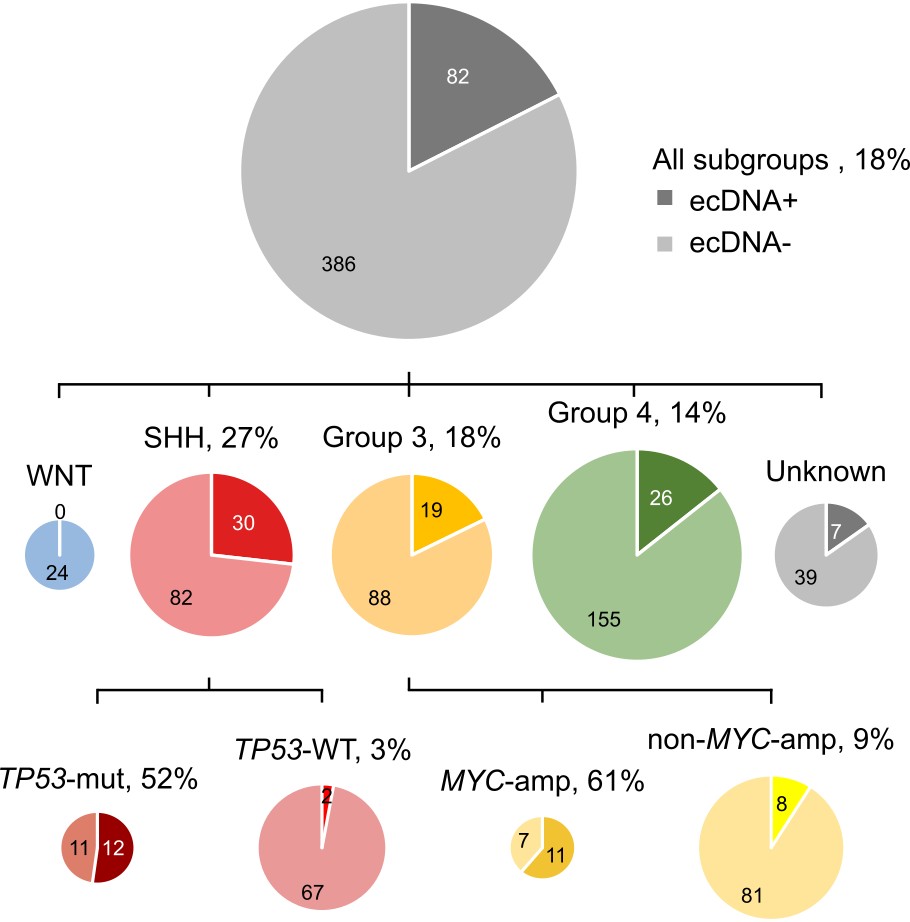
\includegraphics[]{figures/1-1.png}
    \caption[Presence of ecDNA by molecular subgroup across 468 MB patient tumors.]{\textbf{Presence of ecDNA by molecular subgroup across 468 MB patient tumors.} \textit{TP53}-mut/WT: \textit{TP53}-mutant/wild-type. \textit{MYC}-amp: \textit{MYC} copy number $\geq 5$ estimated from \gls{wgs}.}  
    \label{fig:1a}
\end{figure}

\begin{figure}[!h]
    \centering
    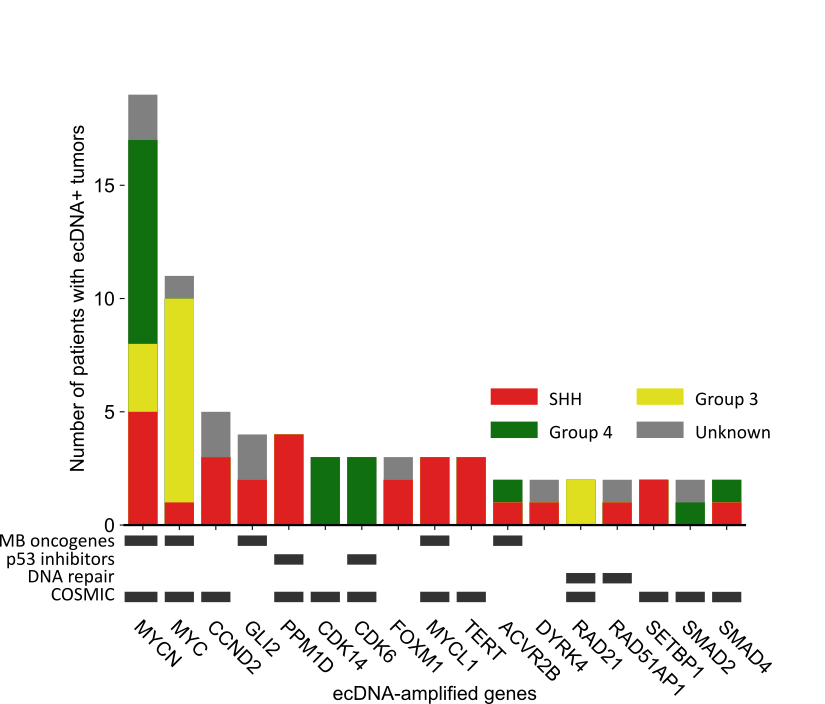
\includegraphics[]{figures/1-2.png}
    \caption[Recurrently amplified genes on ecDNA in MB.]{\textbf{Recurrently amplified genes on ecDNA in MB.} A subset of recurrently ($n \geq 2$) amplified genes on ecDNA in this patient cohort. p53 inhibitors: negative regulators of p53 pathway activity; COSMIC: genes listed as tier 1 or 2 of the COSMIC Cancer Gene Census \cite{cosmic}.}
    \label{fig:1b}
\end{figure}

\subsection{ecDNA predicts poor prognosis in medulloblastoma.}
To evaluate ecDNA as a potential prognostic marker in MB, we performed survival analyses across patients for whom clinical metadata were available. Patients with \gls{ecDNA+} tumors had significantly worse overall and progression-free 5-year survival (OS, PFS) compared to patients with ecDNA-negative tumors (ecDNA-) (log-rank test, $p < 0.005$; Fig. \ref{fig:km}). Stratified by molecular subgroup, ecDNA+ patients had worse overall survival in the SHH, Group 3 and Group 4 MB subgroups ($p<0.05$ for all subgroups; Fig. \ref{fig:km-subgroup}). Survival of WNT subgroup patients was not analyzed because no WNT tumors in our patient cohort were ecDNA+. To determine whether ecDNA+ patients had worse outcomes than patients with tumors harboring other types of focal somatic copy number amplification (fSCNA), we stratified patients by the topology of the amplification(s) present in the tumor genomes, using previously published methods \cite{Kim_2020}. As expected, ecDNA+ patients had the poorest clinical outcomes, significantly worse compared to patients without fSCNAs or with linear amplifications ($p<0.005$, Fig. \ref{fig:km-cna}). 

\begin{figure}[!h]
    \centering
    \begin{subfigure}{0.49\textwidth}
        \centering
        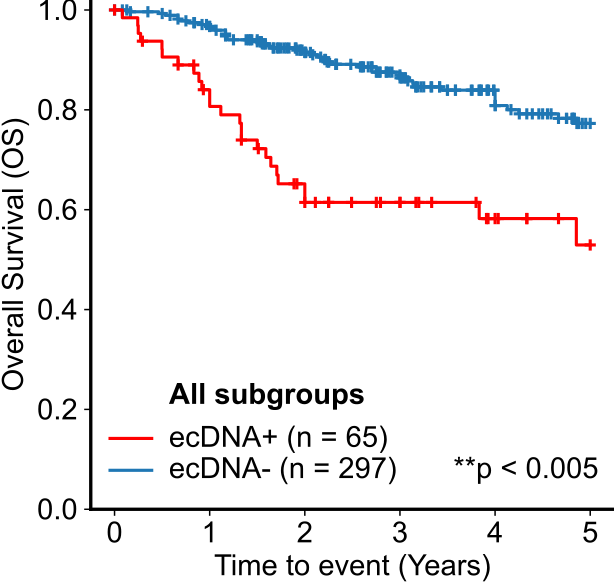
\includegraphics{p-KM-OS}
        \caption{}
        \label{subfig:os}
    \end{subfigure}
    \begin{subfigure}{0.49\textwidth}
        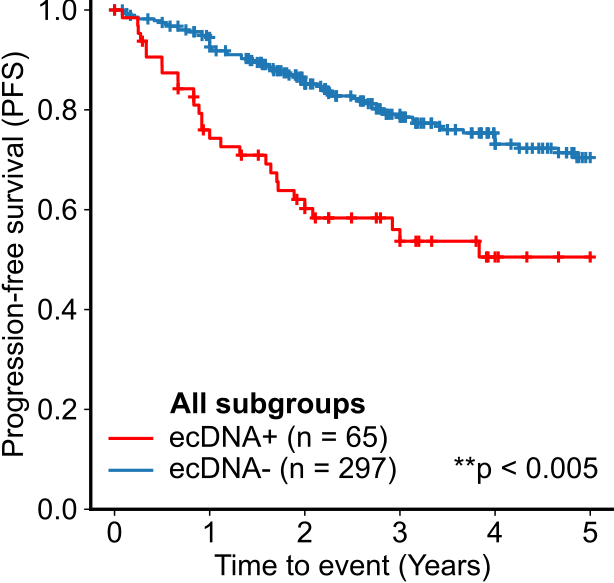
\includegraphics{p-KM-PFS}
        \caption{}
        \label{subfig:pfs}
    \end{subfigure}
    \caption[Survival of ecDNA+ and ecDNA- MB patients.]{\textbf{Survival of ecDNA+ and ecDNA- MB patients.} (\textbf{a}) 5-year overall survival and (\textbf{b}) progression-free survival of ecDNA+ and ecDNA- MB patients.}
    \label{fig:km}
\end{figure}

\begin{figure}[!h]
    \centering
    \begin{subfigure}{0.32\textwidth}
        \centering
        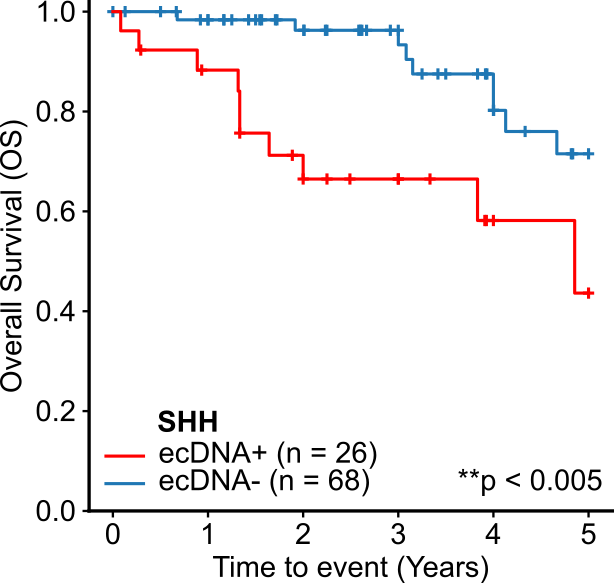
\includegraphics{p-KM-OS-SHH}
        \caption{}
        \label{subfig:os-shh}
    \end{subfigure}
    \begin{subfigure}{0.32\textwidth}
        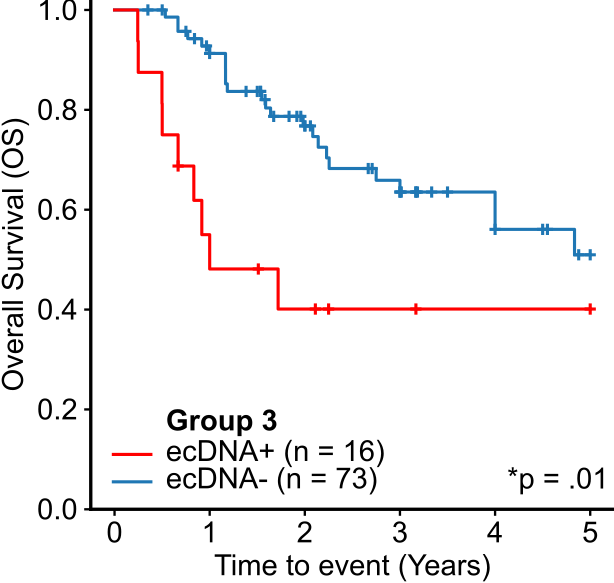
\includegraphics{p-KM-OS-G3}
        \caption{}
        \label{subfig:os-g3}
    \end{subfigure}
    \begin{subfigure}{0.32\textwidth}
        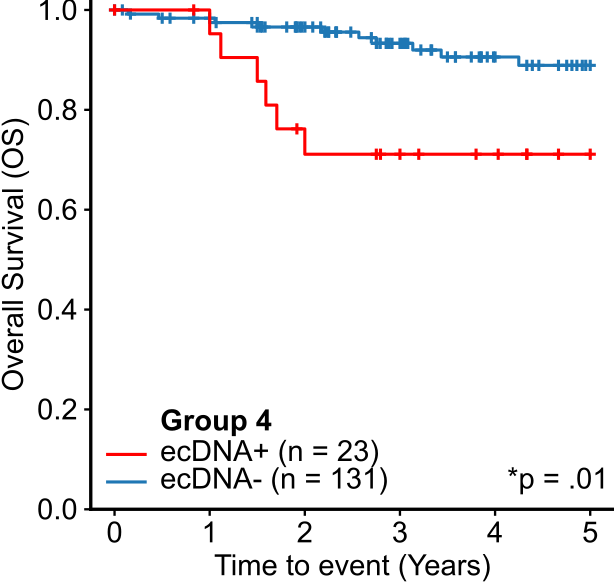
\includegraphics{p-KM-OS-G4}
        \caption{}
        \label{subfig:os-g4}
    \end{subfigure}
        \begin{subfigure}{0.32\textwidth}
        \centering
        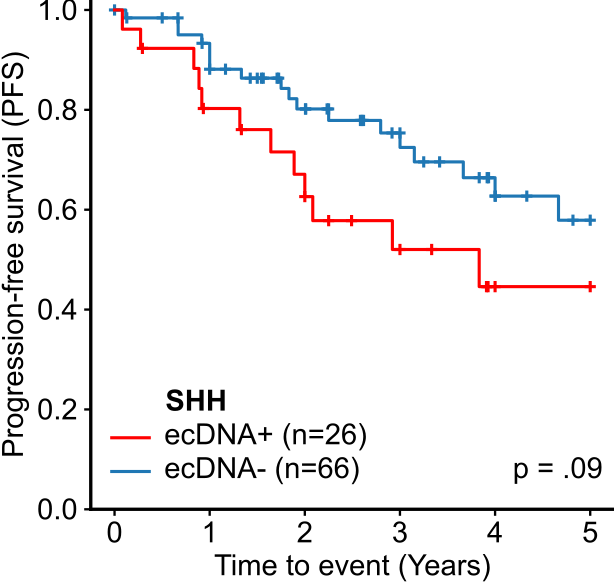
\includegraphics{p-KM-PFS-SHH}
        \caption{}
        \label{subfig:pfs-shh}
    \end{subfigure}
    \begin{subfigure}{0.32\textwidth}
        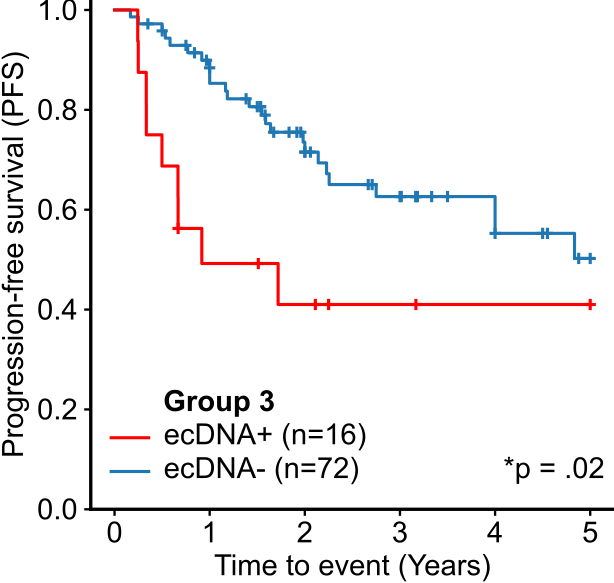
\includegraphics{p-KM-PFS-G3}
        \caption{}
        \label{subfig:pfs-g3}
    \end{subfigure}
    \begin{subfigure}{0.32\textwidth}
        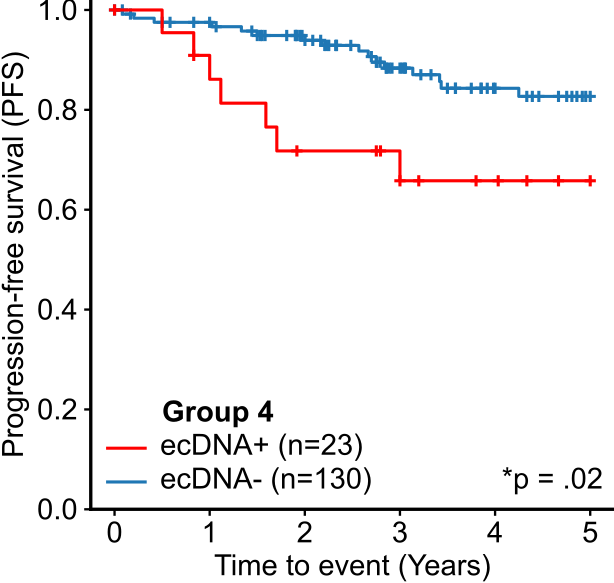
\includegraphics{p-KM-PFS-G4}
        \caption{}
        \label{subfig:pfs-g4}
    \end{subfigure}
    \caption[Survival of ecDNA+ and ecDNA- MB patients, stratified by molecular subgroup.]{\textbf{Survival of ecDNA+ and ecDNA- MB patients, stratified by molecular subgroup.} Survival curves indicating (\textbf{a-c}) 5-year overall survival and (\textbf{d-f}) progression-free survival of ecDNA+ and ecDNA- MB patients. \textbf{a-b}: SHH. \textbf{c-d}: Group 3. \textbf{e-f}: Group 4. WNT subgroup was not analyzed because ecDNA was not detected in WNT MB tumors.}
    \label{fig:km-subgroup}
\end{figure}

\begin{figure}[!h]
    \centering
    \begin{subfigure}{0.49\textwidth}
        \centering
        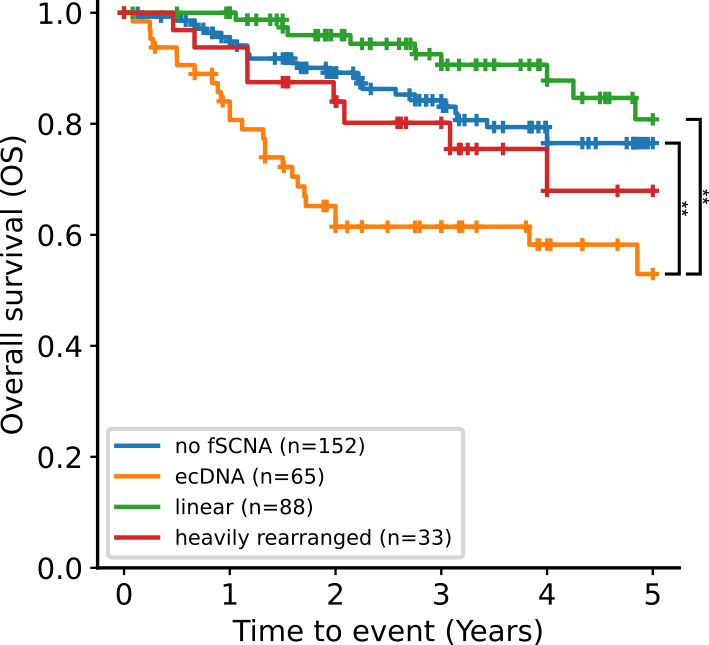
\includegraphics{p-KM-OS-subtypes}
        \caption{}
        \label{subfig:}
    \end{subfigure}
    \begin{subfigure}{0.49\textwidth}
        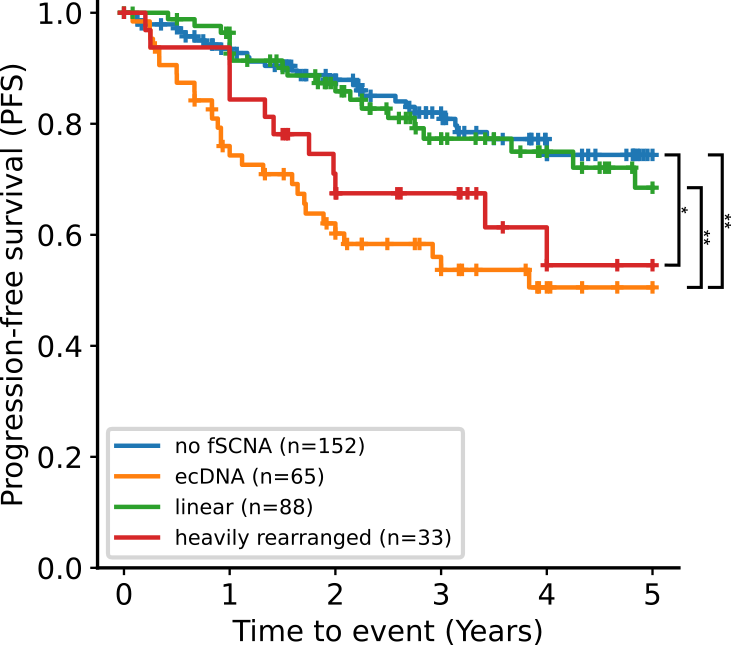
\includegraphics{p-KM-PFS-subtypes}
        \caption{}
        \label{subfig:}
    \end{subfigure}
    \caption[Survival of ecDNA+ and ecDNA- MB patients, stratified by focal somatic amplification(s) present.]{\textbf{Survival of ecDNA+ and ecDNA- MB patients, stratified by focal somatic amplification(s) present} in the tumor as classified by AmpliconClassifier \cite{Kim_2020}. ecDNA: tumor harbors a circular extrachromosomal amplification. Heavily rearranged: Tumor harbors an amplification classified as complex non-cyclic, but no cyclic ecDNA or BFB amplifications. Linear: Tumor harbors a linear amplification, but no highly-rearranged, BFB, or ecDNA amplifications. no fSCNA: no focal somatic copy number amplification detected.}
    \label{fig:km-cna}
\end{figure}

To further estimate the prognostic value of ecDNA, we conducted Cox proportional hazards models controlling for sex, age, and molecular subgroup. Patients with ecDNA+ tumors had greater estimated risk for progression (hazard ratio 2.36, $p < 0.005$) and mortality ($HR = 2.99$, $p < 0.005$) compared to patients with ecDNA- tumors (Fig. \ref{fig:cph-ssa}, Supplementary Table 2 of \cite{Chapman}). 

\begin{figure}[!h]
    \centering
    \begin{subfigure}{0.49\textwidth}
        \centering
        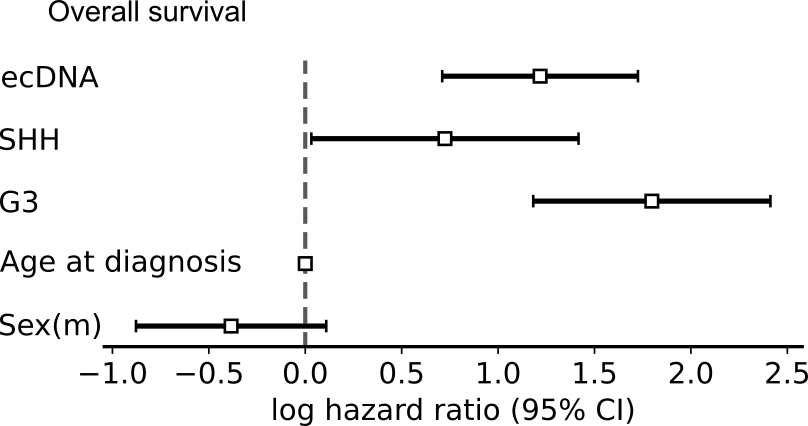
\includegraphics{p-CPH-OS-ssa}
        \caption{}
        \label{fig:cph-os-ssa}
    \end{subfigure}
    \begin{subfigure}{0.49\textwidth}
        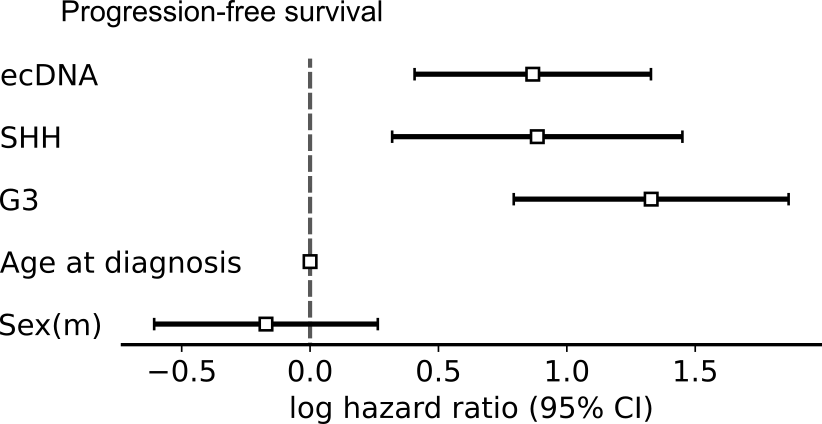
\includegraphics{p-CPH-PFS-ssa}
        \caption{}
        \label{fig:cph-pfs-ssa}
    \end{subfigure}
    \caption[Survival regressions on \gls{ecDNA}, MB subgroup, age and sex.]{\textbf{Survival regressions on \gls{ecDNA}, MB subgroup, age and sex.} Log hazard ratios for ecDNA status, MB subgroup, age and sex estimated by Cox proportional hazards regression on (\textbf{a}) overall survival and (\textbf{b}) progression-free survival. Model was fitted using \gls{mle}. Bars indicate 95\% confidence intervals. Estimated hazard ratios for ecDNA are $HR_{OS} = 2.99$, $p < 0.005$ and $HR_{PFS} = 2.36$, $p < 0.005$. }
    \label{fig:cph-ssa}
\end{figure}

\subsection{\textit{TP53} alterations are associated with ecDNA in SHH MB tumors.}
The tumor suppressor protein p53 (\textit{TP53}) is involved in DNA damage sensing, cell cycle arrest and apoptosis, and is frequently affected by somatic mutations and pathogenic germline variants in SHH MB \cite{Ramaswamy_2016, li-fraumeni_1988, waszak_2018}. Moreover, SHH-subgroup MBs with inactivating \textit{TP53} mutations are known to be associated with chromothripsis \cite{Rausch_2012}, a process of catastrophic shattering of a chromosome that has been shown to precede ecDNA formation in cell line models \cite{shoshani_2020, umbreit_2020}. To test whether \textit{TP53} mutations were associated with the presence of ecDNA in MB, we accessed the somatic and germline \textit{TP53} mutation status available for 92 SHH MBs. We found significant enrichment of \textit{TP53} alterations in ecDNA+ SHH MB tumors (12 of 23, 52\%) compared to ecDNA- SHH MB tumors (2 of 69, 3\%; $p=1.3e-7$, Fisher exact test; Table \ref{tab:shh-tp53}). We did not find a significant association between \textit{TP53} alterations and ecDNA either in the other MB subgroups or across the entire MB cohort, suggesting that in MB, a possible functional relationship between \textit{TP53} alterations and ecDNA is restricted to the SHH subgroup. 

%%%% TABLE 1 %%%%
\begin{table}[!ht]
\caption[\textit{TP53} mutation is associated with ecDNA in SHH subgroup MBs.]{\textbf{\textit{TP53} mutation is associated with ecDNA in SHH subgroup MBs.} We acquired somatic and germline mutation status of 92 SHH MBs from our patient cohort. Nearly every \textit{TP53}-mutant patient tumor contained ecDNA (12/14). The two without ecDNA showed evidence of breakage-fusion-bridge (BFB) amplification, a hypothesized precursor to ecDNA formation.}
\begin{center}
\begin{tabular}{ p{1in} p{1in} p{1in} }
\hline
 & \gls{ecDNA+} & ecDNA- \\
\hline
\textit{TP53}\textsubscript{mut} & 12 & 2 \\
\textit{TP53}\textsubscript{WT} & 11 & 67 \\
\hline
\end{tabular}
\end{center}
\label{tab:shh-tp53}
\end{table}

\par We hypothesized that the established effect of p53 mutation on SHH MB patient survival \cite{zhukova_2013} may be mediated, at least partially, by ecDNA (Fig. \ref{fig:aft}). To test this, we conducted mediation analyses using the Baron Kenny approach \cite{baron-kenny_1986}. Briefly, variable $M$ (ie, ecDNA status) is considered a mediator of the effect of independent variable $X$ (ie, p53 mutation) on outcome $Y$ (ie, patient survival) if (1) $X$ significantly predicts $Y$; (2) $X$ significantly predicts $M$; and (3) in a multiple regression of $Y$ on $X$ and $M$, $M$ significantly predicts $Y$ and the effect of $X$ on $Y$ is reduced relative to (1) (Fig. \ref{subfig:aft-model}) \cite{jung_2012}. To test (1), we fitted a log-normal \gls{aft} regression of \gls{pfs} parameterized on age, sex, molecular subgroup and p53 mutation status, using \gls{mle}. Without information on ecDNA, this model estimates that p53 mutation significantly reduces survival time by 77\% ($\mu = -1.46$, $p < 0.005$, Wald test; Fig. \ref{subfig:aft-p53}). For (2), we have already shown that p53 mutation strongly predicts the presence of ecDNA given molecular subgroup. To test (3), we refitted our AFT model parameterized on age, sex, molecular subgroup, p53 mutation, and ecDNA status. This model estimates that ecDNA significantly reduces survival time by 56\% ($\mu = -0.81$, $p < 0.005$; Fig. \ref{subfig:aft-p53-ecdna}). The same model estimates an insignificant reduction in survival time for p53 mutation, with a coefficient of lesser magnitude than that of (1) ($\mu = -0.94$, $p = 0.06$). We therefore concluded that the known prognostic effect of p53 mutation on survival may be partially  explained by an effect of ecDNA on prognosis and by the frequent co-occurrence of ecDNA in p53-mutant tumors.

\begin{figure}[!h]
    \centering
    \begin{subfigure}{\textwidth}
        \centering
        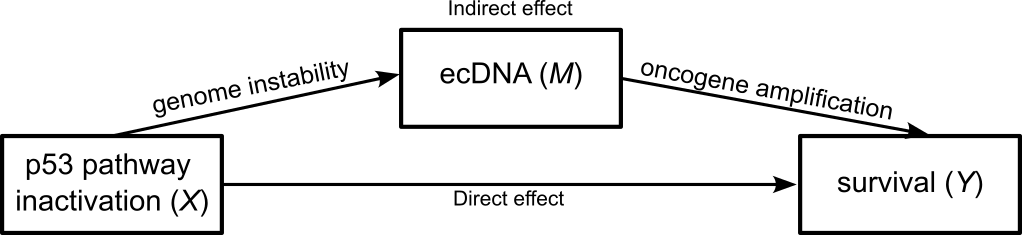
\includegraphics{1-4-1-mediation}
        \caption{}
        \label{subfig:aft-model}
    \end{subfigure}
    \centerline{%
    \begin{subfigure}{0.55\textwidth}
        \centering
        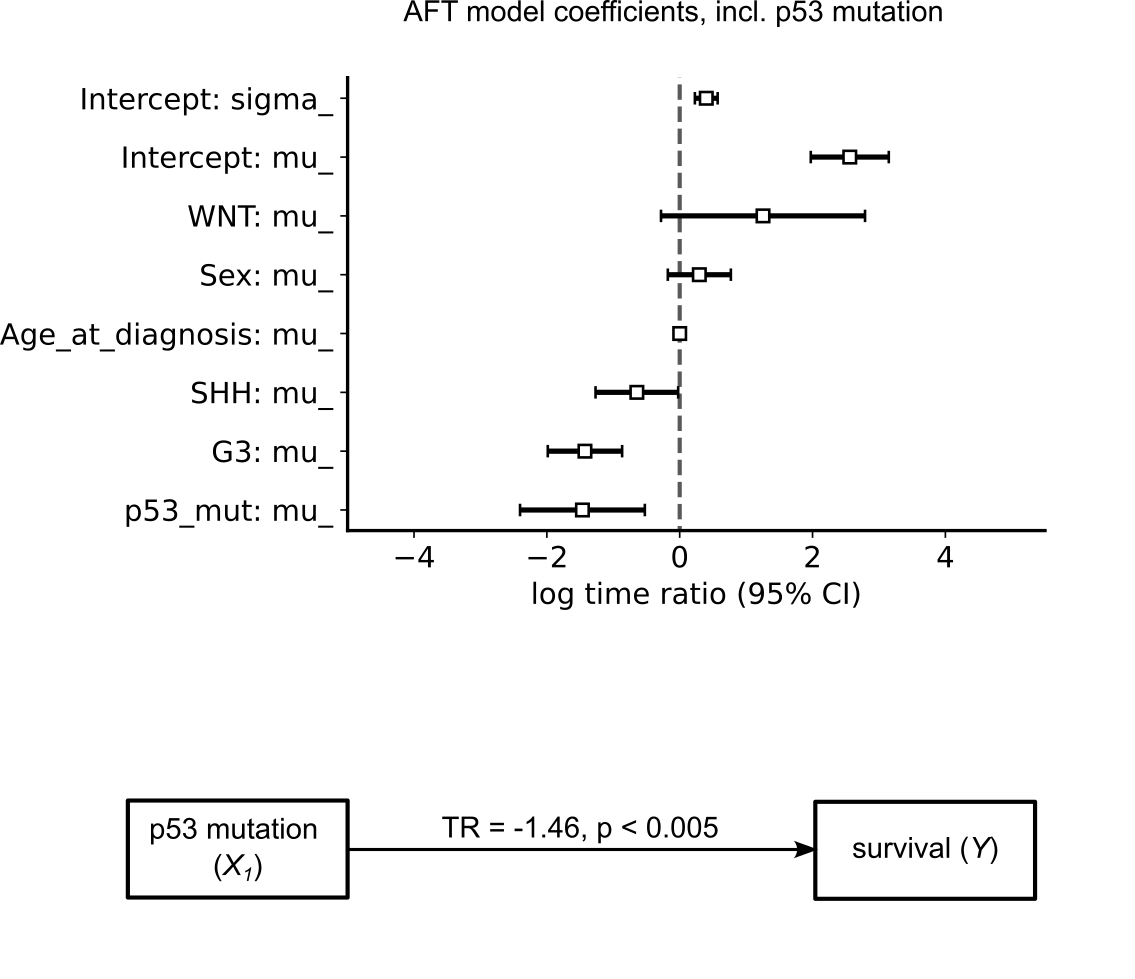
\includegraphics{p-AFT-PFS-p53}
        \caption{}
        \label{subfig:aft-p53}
    \end{subfigure}
    \begin{subfigure}{0.55\textwidth}
        \centering
        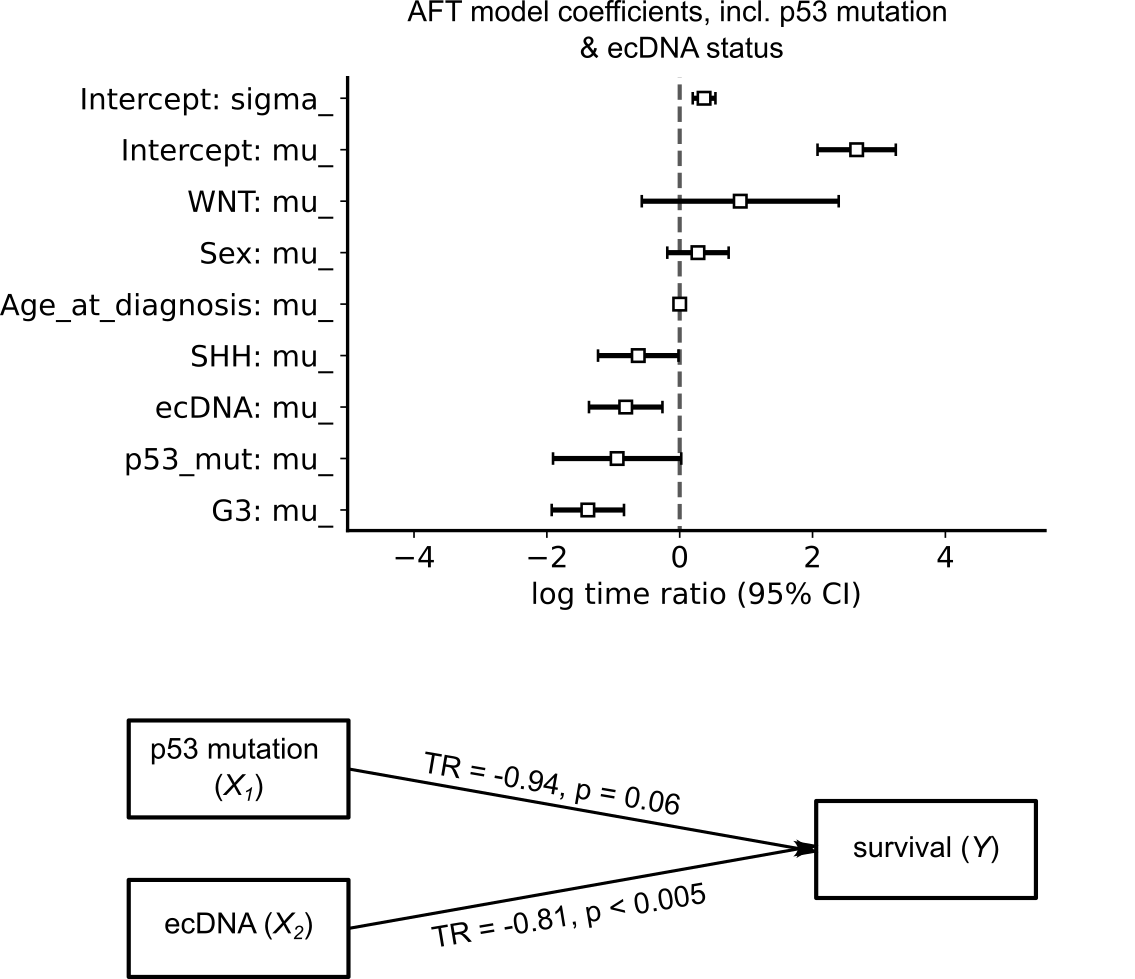
\includegraphics{p-AFT-PFS-p53-ecDNA}
        \caption{}
        \label{subfig:aft-p53-ecdna}
    \end{subfigure}%
    }
    \caption[Classical mediation analysis of associations between p53 mutation, \gls{ecDNA}, and patient outcomes.]{\textbf{Mediation analysis of p53 mutation, ecDNA, and progression-free survival.} (\textbf{a}) Model diagram of the proposed mediation relationship. p53 inactivation may predispose a tumor to form ecDNA, which then affects survival; p53 may also have ecDNA-independent effects on survival, eg. by formation of other structural variants. (\textbf{b}) Top: estimated time ratios for effects of age, sex, molecular subgroup and p53 mutation on \gls{pfs}. Bottom: effect size and p-value for p53 mutation are illustrated in the diagram below. (\textbf{c}) Top: estimated time ratios for effects of age, sex, molecular subgroup, p53 mutation, and ecDNA on \gls{pfs}. Bottom: effect size and p-values for p53 mutation and ecDNA are illustrated in the diagram below. The effect size of p53 on survival is decreased when controlling for ecDNA as a covariate, suggesting that ecDNA partially mediates the effect of p53 on survival.}
    \label{fig:aft}
\end{figure}

\par To evaluate whether there is a \textit{TP53}-independent effect of ecDNA on survival, we performed Cox regression including \textit{TP53} alteration as a covariate and controlling for collinearity. The effect of ecDNA on survival remains significant but diminished when we include p53 alteration as a covariate in our Cox models ($HR_{PFS} = 1.87, p = 0.01$; $HR_{OS} = 2.32, p < 0.005$; Fig. \ref{fig:cph-ssap}), indicating that there is an effect of ecDNA on survival that cannot be explained by p53 mutation alone. Such an effect may be explainable by a p53-independent mechanism of ecDNA formation, or by inactivation of the p53 pathway by other means such as \textit{CDKN2A} deletion or \textit{PPM1D}, \textit{CDK6}, \textit{MDM4} or \textit{MDM2} amplification \cite{mclendon_2008}. Although causality cannot be inferred from these data alone, our survival analyses identify \textit{TP53} alteration and ecDNA as clinically relevant biomarkers for a subset of highly aggressive SHH MB tumors. 

\begin{figure}[!h]
    \centering
    \centerline{%
    \begin{subfigure}{0.55\textwidth}
        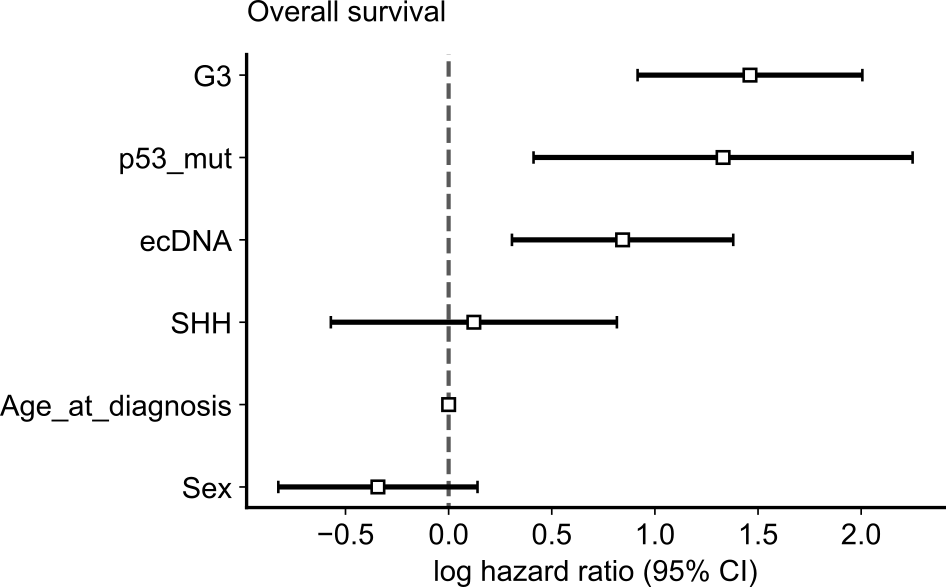
\includegraphics[right]{p-CPH-OS-ssap}
        \caption{}
        \label{subfig:cph-os-ssap}
    \end{subfigure}
    \begin{subfigure}{0.55\textwidth}
        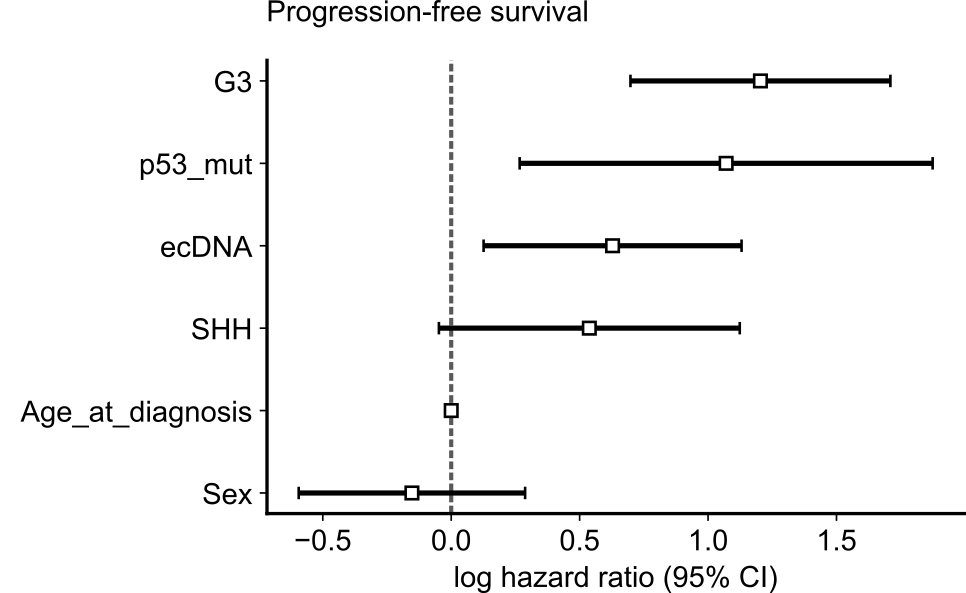
\includegraphics[left]{p-CPH-PFS-ssap}
        \caption{}
        \label{subfig:cph-pfs-ssap}
    \end{subfigure}%
    }
    \caption[Survival regressions on \gls{ecDNA} status, MB subgroup, age, sex, and p53 mutation.]{\textbf{Survival regressions on \gls{ecDNA} status, MB subgroup, age, sex, and p53 mutation.} Log hazard ratios for ecDNA status, MB subgroup, age, sex, and p53 mutation estimated by Cox proportional hazards regression on (\textbf{a}) overall survival and (\textbf{b}) progression-free survival. Model was fitted using ridge regression to control for collinearity. Bars indicate 95\% confidence intervals. Estimated hazard ratios for ecDNA are $HR_{OS} = 2.32, p < 0.005$; $HR_{PFS} = 1.87, p = 0.01$. }
    \label{fig:cph-ssap}
\end{figure}

\section{Discussion}

\par As in other cancers \cite{Turner_2017,Kim_2020,luebeck_2022}, ecDNA frequently amplifies known oncogenic MB driver genes. Our results identify ecDNA as a frequent feature of \textit{MYC}-amplified Group 3 and p53-mutant SHH tumors, which share exceptionally poor prognoses \cite{Ryan_2012,Rausch_2012} but few other recurrent driver mutations. Recent longitudinal analysis of Barrett’s esophagus suggests that \textit{TP53} alteration is an early event in ecDNA-driven malignant transformation \cite{luebeck_2022}. However, the absence of detectable ecDNA in \textit{TP53}-mutant WNT subgroup tumors, and the frequent occurrence of ecDNA in Group 3 tumors with wild type \textit{TP53}, suggest that the mechanisms for the generation and selection of tumor cells with ecDNA are MB subgroup-specific and thus may be modulated by the different cellular contexts of MB progenitor cells.

\par A long-standing problem in the clinical management of medulloblastoma tumors has been the paucity of effective targeted molecular treatments for MB, especially in relapsed cases. For example, the SMO inhibitor vismodegib, one of few targeted drugs approved for SHH medulloblastoma, is ineffective against \textit{TP53}-mutant, \textit{MYCN}-amplified or \textit{GLI2}-amplified tumors \cite{robinson_2015}, each a recurrent feature of ecDNA+ MB in our patient cohort. Through a retrospective analysis of one of the largest cohorts of \gls{wgs} and clinical outcome data from MB patients assembled to date, we demonstrate that the occurrence of ecDNA significantly associates with poor outcome across the entire cohort and within individual MB subgroups. Our survival analysis estimates that relative to ecDNA- patients, ecDNA+ MB patients are more than twice as likely to relapse and three times as likely to die during the follow-up interval. The identification of MB patients with ecDNA is therefore crucial to pave the way for precision medicine approaches targeting ecDNA-specific properties.

\section{Methods}
\label{chap1:methods}
\subsection{Statistical methods}
Statistical test, test statistic and p-values are indicated where appropriate in the main text. Categorical associations were established using the chi-squared test of independence if $N>5$ for all categories, and Fisher exact test otherwise. For both tests, the python package scipy.stats v1.5.3 implementation was used \cite{scipy}. Multiple hypothesis corrections were performed using the Benjamini-Hochberg correction \cite{bh} implemented in statsmodels v0.12.0 \cite{statsmodels}. All statistical tests described herein were two-sided unless otherwise specified.

\subsection{Medulloblastoma WGS}
Paired-end whole genome sequencing (WGS) data were acquired for each of the sources described below. In total the WGS cohort comprised 468 patients, 4 cell lines and 26 PDX models. Unless otherwise specified, WGS was acquired for 1 tumor biosample per patient.

\subsubsection{CBTN -- Children's Brain Tumor Network (114 biosamples from 101 patients)} WGS of medulloblastoma tumor biopsies were identified using the Gabriella Miller KidsFirst Data Resource center portal (\url{https://portal.kidsfirstdrc.org/}) on 29 May 2020. Patients were originally sequenced as part of the Pediatric Brain Tumor Atlas (PBTA) (\url{https://cbtn.org/pediatric-brain-tumor-atlas}). WGS data were preprocessed and aligned using the KidsFirst harmonized WGS pipeline (hg38) and subsequently analyzed using Cavatica (\url{https://cavatica.sbgenomics.com/}), on the cloud genomic analysis platform for KidsFirst genomic data. Docker containers containing fingerprint and AmpliconArchitect software were installed on the Cavatica cloud genomics platform (see Methods: ``EcDNA detection and classification").

\subsubsection{St Jude (79 patients)} WGS of MB biopsies were identified using the St Jude Cloud Data Portal (\url{https://platform.stjude.cloud/data/}) on 11 February 2020. WGS was preprocessed and aligned by bwa-mem to hg38 as described in McLeod et al31. Docker containers of fingerprint and AmpliconArchitect software were installed on the DNANexus cloud genomics platform (see Methods: ``EcDNA detection and classification").
\subsubsection{ICGC - International Cancer Genome Consortium (237 patients)} WGS of MB tumor biopsies was identified using the ICGC Data Portal (\url{https://dcc.icgc.org/}) on 12 May 2020 and downloaded from the Collaboratory cloud genomics platform using the ICGC Score download client. These tumor genomes were previously sequenced, aligned and deposited with ICGC in other publications (GRCh37)\cite{Northcott_2017,pcawg}.

\subsubsection{Archer \textit{et al.} (43 patients)} All WGS data for these 43 patients were previously published elsewhere\cite{Northcott_2017}. Sequencing data were aligned to human genome reference GRCh37 processed according to the best practice pipelines at the Cancer Genome Analysis group at the Broad Institute\cite{archer_2017}.

\subsubsection{Rady Children's Hospital (8 patients)} Tumor biopsies were collected and consented for research as part of the Rady Molecular Tumor Board (MTB). Paired end reads were acquired from Rady's Children hospital. Sequencing depth for all samples were at least 30x. Raw fastq reads were aligned to UCSC hg38 coordinates using BWA v0.7.17-r1188 \cite{bwa}.  Reads were sorted by samtools v0.1.19 \cite{samtools}, marked for duplicates with Picard Tools v2.12.3, and recalibrated with GATK v3.8-1-0 \cite{mckenna_2010,depristo_2011,vanderauwera_2013}.

\subsubsection{Cell lines and PDX models (4 cell lines, 26 PDXs)} Low-coverage WGS for 19 PDX models and 9 corresponding origin human tumors were obtained from a previous publication \cite{rusert_2020}. An additional 6 PDX biosamples (RCMB25, RCMB32, RCMB56, RCMB57, RCMB58 and RCMB69) were contributed by Wechsler-Reya lab using similar methods to establish PDX lines. Cell lines (D283, D341, D425 and D458) were contributed by Bagchi (SBP), Taylor (U. Toronto) and Wechsler-Reya (SBP) labs. WGS was performed at the UCSD IGM Genomics and Sequencing Core (hg38) for all samples except D283, for which no WGS was obtained. Preprocessing and alignment was performed using the same protocol as the RCH patient biopsies above.
\subsection{ecDNA detection and classification from bulk WGS}
To detect ecDNA, all samples in the WGS cohort were analyzed using AmpliconArchitect \cite{AA} v1.2 and AmpliconClassifier \cite{Kim_2020} v0.4.4. Briefly, the AmpliconArchitect algorithm was performed as follows. Copy number segmentation and estimation were performed using CNVkit v0.9.6 \cite{cnvkit}. Segments with copy number $\geq 4$ were extracted using AmpliconSuite-pipeline (April 2020 update) as ``seed" regions. For each seed, AmpliconArchitect searches the region and nearby loci for discordant read pairs indicative of genomic structural rearrangement. Genomic segments are defined based on boundaries formed by genomic breakpoint locations (identified by discordant reads) and by modulations in genomic copy number. A breakpoint graph of the amplicon region is constructed using the CN-aware segments and the genomic breakpoints, and cyclic paths are extracted from the graph.  Amplicons are classified as ecDNA, breakage-fusion-bridge, complex, linear, or no focal amplification by the heuristic-based companion script, AmpliconClassifier. Biosamples with one or more classifications of ``ecDNA" were considered potentially ecDNA+, and all others were considered ecDNA- (Supplementary Table 1c from \cite{Chapman}). We manually reviewed all potential ecDNA+ assembly graphs and reclassified those with inconclusive ecDNA status, which we defined as any of the following:
\begin{itemize}
    \item Low-copy amplification ($<5$) AND no copy number change at discordant read breakpoints
    \item Cycles consisting of the repetitive region at chr5:820000 (GRCh37).
\end{itemize}
Code is available at:
\begin{itemize}
    \item AmpliconSuite-pipeline: \url{https://github.com/jluebeck/AmpliconReconstructor}
    \item AmpliconArchitect: {https://github.com/jluebeck/AmpliconArchitect} 
    \item AmpliconClassifier: \url{https://github.com/jluebeck/AmpliconClassifier} 
\end{itemize}
The ecDNA- status of the D283 cell line was not determined computationally by WGS, but by copy number analysis of DNA methylation, FISH (see Methods: ``FISH").
\subsection{Fingerprinting analysis}
To uniquely identify WGS from each patient, we counted reference and alternate allele frequencies at 1000 variable non-pathogenic SNP locations in the human genome according to the 1000 Genomes project \cite{1000_genomes}, and performed pairwise Pearson correlation between all WGS samples. Biospecimens originating from the same patient tumor (eg., primary/relapse or origin/PDX pairs) were readily distinguishable by high correlation across these sites ($r > 0.80$). We identified one case in our cohort in which 2 tumor biosamples had highly correlated fingerprints: MDT-AP-1217.bam and ICGC\_MB127.bam. We arbitrarily removed ICGC\_MB127 from the patient cohort. 
\subsection{Patient metadata, survival, and medulloblastoma subgroup annotation.}
Where available, patient samples and models were assigned metadata annotations including age, sex, survival, and MB subgroup based on previously published annotations of the same tumor or model \cite{archer_2017,Northcott_2017,waszak_2018,rusert_2020,ivanov_2016,robinson_2012,northcott_2012}. Sample metadata are also available in some cases from the respective cloud genomics data platform: \url{https://dcc.icgc.org/} (ICGC), \url{https://pedcbioportal.kidsfirstdrc.org/} and \url{https://portal.kidsfirstdrc.org/} (CBTN), and \url{https://pecan.stjude.cloud/} (St Jude). Where primary sources disagreed on a metadata value, that value was reassigned to NA. Patient tumors from the CBTN were assigned molecular subgroups based on consensus of 2 molecular classifiers using RSEM-normalized FPKM data: MM2S \cite{gendoo_2016} and the D3b medulloblastoma classifier at the Children's Hospital of Philadelphia (\url{https://github.com/d3b-center/medullo-classifier-package}). To determine molecular subgroup of PDX samples, we generated or obtained from a previous publication \cite{rusert_2020} DNA methylation profiles (Illumina 450k or EPIC) and classified samples by molecular subgroup according to the DKFZ brain tumor methylation classifier (\url{https://www.molecularneuropathology.org/mnp}) \cite{Northcott_2017}.
\subsection{\textit{TP53} mutation annotation}
\subsubsection{Somatic mutations} Somatic \textit{TP53} mutation information for the ICGC and CBTN cohorts was acquired from a previous publication \cite{waszak_2018} and from the ICGC and CBTN data portals (see Methods\: "Patient metadata, survival, and subgroup annotation". Somatic \textit{TP53} mutation information for the St. Jude cohort was extracted from the standard internal St. Jude variant calling pipeline \cite{stjude}. Somatic mutations were only considered which were protein-coding and missense, nonsense, insertion or deletion, or affected a splice site junction.

\subsubsection{Germline variants} Whole-genome sequencing (WGS) GVCF files were downloaded from the ICGC data portal (\url{https://dcc.icgc.org/}), the KidsFirst data portal (\url{https://portal.kidsfirstdrc.org/dashboard}) and DNAnexus for St. Jude Pediatric Cancer Genome Project (PCGP). xGVCF files were merged with GLnexus \cite{glnexus} and converted to PLINK format for analysis of ICGC, PCGP and KidsFirst genotypes. PCGP genotypes were converted to hg19 coordinates using liftover. Variants from \textit{TP53} genomic locus (hg19\:chr17\:7571739-759080) were extracted and annotated with REVEL \cite{revel_2016}, CADD \cite{cadd}, ClinVar (accessed June 2021) and Variant Effect Predictor (VEP) \cite{vep}. REVEL GRCh38 scores were downloaded from \url{https://sites.google.com/site/revelgenomics/} (date accessed: 03/05/2021). CADDv1.6 scores were downloaded from \url{https://cadd.gs.washington.edu/info} (date accessed: 03/23/2020). VEP scores were calculated with \url{http://grch37.ensembl.org/index.html} release 104 (date accessed: 04/27/21). Clinvar scores were obtained from \url{https://ftp.ncbi.nlm.nih.gov/pub/clinvar/vcf_GRCh37/} (Date accessed: 04/27/21). VEP variants considered pathogenic included "frameshift" and ``splice" variants. ClinVar annotations considered pathogenic included ``frameshift", ``stop", ``splice", and ``deletion", and whose clinical significance were ``pathogenic" or ``likely pathogenic". CADD ``pathogenic" variants had a CADD score of at least 10 (Phred score). REVEL ``pathogenic" variants had a REVEL score of at least 0.5. Only variants with minor allele frequency (MAF) less than 5\%, according to the gnomAD r2.1.1 database, were analyzed \cite{karczewski_2020}.

\subsection{Survival analyses}
\acrfull{km}, \acrfull{cph}, and \acrfull{aft} analyses were performed with Lifelines v0.26.5 \cite{lifelines}. For all analyses, the sample set was all patients annotated with the included covariates; no imputation was performed. 
\subsubsection{Kaplan-Meier} Sample sizes were $n = 362$ (65 ecDNA+; 297 ecDNA-). Differential survival was determined by log-rank test. For \acrshort{km} analyses by class of structural variant, samples were classified as previously described \cite{Kim_2020}. Our sample of patients with breakage-fusion-bridge (BFB) amplification but no ecDNA was too small to test ($n=2$).
\subsubsection{Cox Proportional Hazards on age, sex, molecular subgroup, \& ecDNA} Sample was $n = 352$ observations. Model was fitted by maximum likelihood estimation (MLE).
\subsubsection{Cox Proportional Hazards on age, sex, molecular subgroup, p53 mutation, \& ecDNA} Sample was $n = 322$ observations. Collinearity, \textit{i.e.} strong correlation between predictive variables in a regression model, can result in model instability and unreliable estimation of the collinear coefficients \cite{liu_2017}. To address collinearity between ecDNA and p53 status in our model, we performed ridge estimation of model coefficients \cite{verweij_1994, xue_2007}, determining the ridge penalty parameter $\lambda$ by grid search on 5-fold cross validation of model likelihood on the withheld set.
\subsubsection{Accelerated failure time models and mediation analysis} Mediation analysis was performed using the Baron-Kenny framework \cite{baron-kenny_1986}, following recent best practices \cite{lapointe_2018}. Because of the non-collapsibility of hazard ratios, the proportional hazards assumption and \acrshort{cph} model may not be suitable for mediation analysis in which we need to compare the coefficients with and without the mediator. Thus, we fitted we fitted parametric log-normal \acrshort{aft} regression models as a reasonable alternative to Cox regression. Percent change values reported herein were calculated as
$$\textsc{Percentage Change}=100(e^{\hat{\beta}_k}-1),$$
 where  $\hat{\beta}_k$ is the MLE regression coefficient for random variable $k$ \cite{demeritt_2022}. 

\section{Acknowledgments}

\ackfunding

\par Chapter 1, in full, is adapted from the following manuscript currently being prepared for publication: "Circular extrachromosomal DNA promotes inter- and intratumoral heterogeneity in high-risk medulloblastoma." Chapman, Owen; Luebeck, Jens; Sridhar, Sunita; Wong, Ivy T.L.; Dixit, Deobrat; Wang, Shanqing; Prasad, Gino; Rajkumar, Utkrisht; Pagadala, Meghana; Larson, Jon D.; He, Britney J.; Hung, King L.; Lange, Joshua T.; Dehkordi, Siavash R.; Chandran, Sahaana; Adam, Miriam; Morgan, Ling; Wani, Sameena; Tiwari, Ashutosh; Guccione, Caitlin; Lin, Yingxi; Dutta, Aditi; Lo, Yan Yuen; Juarez, Edwin; Robinson, James T.; Malicki, Denise M.; Coufal, Nicole G.; Levy, Michael; Hobbs, Charlotte; Scheuermann, Richard H.; Crawford, John R.; Pomeroy, Scott L.; Rich, Jeremy; Zhang, Xinlian; Chang, Howard Y.; Dixon, Jesse R.; Bagchi, Anindya; Deshpande, Aniruddha J.; Carter, Hannah; Fraenkel, Ernest; Mischel, Paul S.; Wechsler-Reya, Robert J.; Bafna, Vineet; Mesirov, Jill P.; Chavez, Lukas. The dissertation author was the primary investigator and author of the manuscript.

%%%%%%%%%%%%%%%%%%%%
\chapter{\singlecelltitle}
\label{chap:heterogeneity}
\glsresetall
\clearpage

\section{Abstract}
\par\textit{Motivation ---} Intratumoral copy number heterogeneity of \gls{ecDNA} in single cells of a tumor is widely believed to contribute to tumor evolution and drug resistance. The capacity to count ecDNA in a large number of single cells would enable the observation of this heterogeneity in sequential tumor biopsies, revealing the population dynamics of ecDNA under therapeutic selection. Numerous algorithms have been developed to estimate genomic copy number from single-cell sequencing data. However, none are designed to quantify ecDNA copy number from single-cell profiles of accessible chromatin (scATAC-seq).
\par\textit{Results ---} To estimate the copy number of a known ecDNA sequence from scATAC-seq data, we compare sequencing read coverage at the ecDNA locus to that elsewhere in the genome. \gls{ecDNA} copy number estimated by this approach strongly correlates to transcriptional measures of ecDNA activity. We apply our method to a dataset of multiome single cell ATAC + Gene Expression (scRNA+ATAC-seq) data from the primary human tumor (HT) and patient-derived xenograft (PDX) of a p53-mutant, SHH subgroup medulloblastoma (MB), and show that \gls{ecDNA+} cells were strongly selected during PDX model establishment. We orthogonally validate our model by estimating ecDNA copy number in the same tumor using automated image analysis on FISH imaging of interphase nuclei stained for ecDNA.
\par\textit{Availability and implementation ---} A software implementation of our approach is available at \url{ https://github.com/auberginekenobi/ecdna-quant}.

\section{Introduction}
\par Intratumoral copy number heterogeneity of extrachromosomal circular DNA (\gls{ecDNA}) in single cells of a tumor is widely believed to contribute to tumor evolution, drug resistance, and poor patient outcomes \cite{bafna_2022}. In the previous chapter, we detected circular ecDNA by assembling cyclic sequences in short-read \gls{wgs} of bulk patient tissue, enabling us to survey a large retrospective cohort of patient data. However, assembly of bulk \gls{wgs} cannot distinguish variation of ecDNA sequence, copy number, and and gene expression between tumor cells, limiting our capacity to measure intratumoral heterogeneity within a given tumor sample. Therefore, to understand the population dynamics of an ecDNA+ tumor, it is necessary to employ emerging methods to examine ecDNA at single-cell resolution. 
\par To address this challenge, we have applied four orthogonal technologies to the \gls{pdx} MB model tumor RCMB56-pdx. We apply \gls{ogm} and CRISPR-CATCH \cite{crispr-catch} to reconstruct high-confidence sequence assemblies of 2 ecDNA lineages originating from distinct portions of the reference human genome, and show that both sequences are conserved in the corresponding patient tumor RCMB56-ht. Next, we analyze FISH microscopy and single-cell sequencing data to estimate ecDNA copy number amplification at single-cell resolution, and show that a clonal expansion of ecDNA+ cells occurred during the engraftment interim between RCMB56-ht and RCMB56-pdx. We anticipate that similar approaches may shed light on clonal dynamics of ecDNA+ cell populations under other selective pressures such as conventional or targeted therapy.

\section{Results}
\subsection{Linear and circular extrachromosomal amplifications co-exist in the RCMB56 patient tumor and PDX model.}
We have previously described a SHH MB primary tumor with heterozygous somatic \textit{TP53} mutation (\acrshort{rcmb56-ht}) \cite{rusert_2020}, which we have established as a PDX model (\acrshort{rcmb56-pdx}). Analysis of WGS from \acrshort{rcmb56-ht} predicted two distinct amplifications, a circular ecDNA of length 3.2Mbp comprising three regions of chr1 (amp1, Fig. \ref{subfig:rcmb56-ar-1}), and a complex, possibly chromothriptic, 4.5Mbp amplicon comprising 21 segments of chr7 and chr17, with ends mapping to pericentromeric and peritelomeric regions (amp2, Fig. \ref{subfig:rcmb56-ar-2}). Analysis of \gls{wgs} from \acrshort{rcmb56-pdx} confirmed that both focal amplifications were unchanged as compared to the original primary human tumor. To assemble high-confidence sequences for the two amplicons, we performed optical genome mapping (OGM, Bionano Genomics) of \gls{uhmw dna} from \acrshort{rcmb56-pdx}. Assembly from deep \gls{wgs} and \gls{ogm} validated the circular amp1 composed of three DNA segments from chr1 (Fig. \ref{subfig:rcmb56-ar-1}). This analysis also validated the contiguous chromothriptic amplification comprising 21 segments of chr7 and chr17; however, a circular structure could not be conclusively established from \gls{ogm} and \gls{wgs} data (Fig. \ref{subfig:rcmb56-ar-2}). Copy number of amp1 and amp2 was estimated from WGS data at 20 and 10 in \acrshort{rcmb56-ht}, and 30 and 25 in \acrshort{rcmb56-pdx} (Suppl. Figs. 5-6 of \cite{Chapman}). 

\begin{figure}[!h]
    \centering
    \begin{subfigure}{0.49\textwidth}
        \centering
        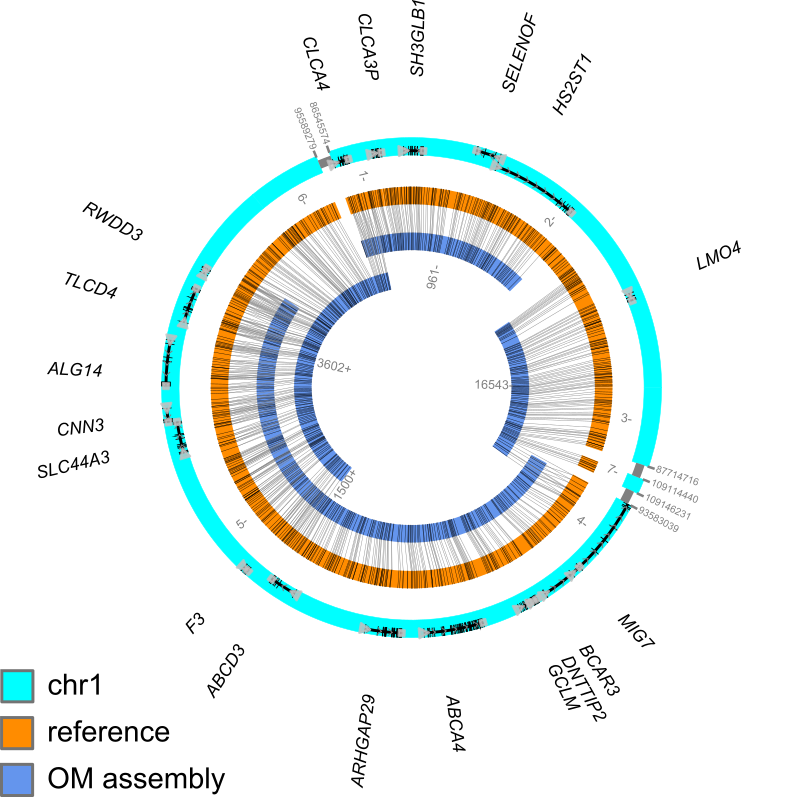
\includegraphics{RCMB56-amp1-AR}
        \caption{}
        \label{subfig:rcmb56-ar-1}
    \end{subfigure}
    \begin{subfigure}{0.49\textwidth}
        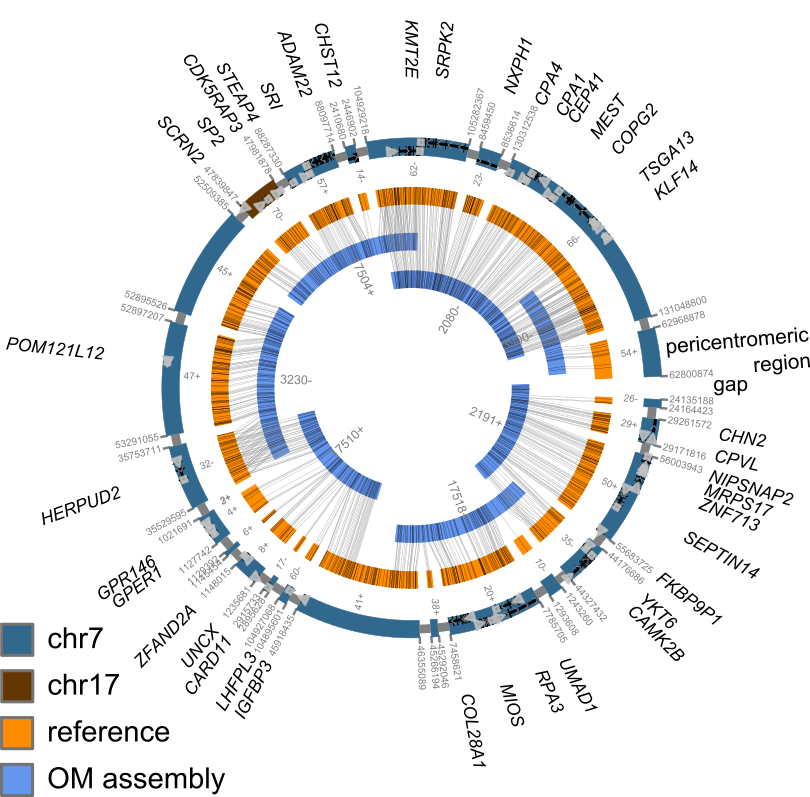
\includegraphics{RCMB56-amp2-AR}
        \caption{}
        \label{subfig:rcmb56-ar-2}
    \end{subfigure}
    \caption[Sequence assemblies of extrachromosomal amplifications in RCMB56.]{\textbf{Sequence assemblies of extrachromosomal amplifications in RCMB56.} (\textbf{a}) RCMB56 amp1 is a circular amplification composed of 3 segments of chr1p. (\textbf{b}) RCMB56 amp2 is a noncircular assembly composed of 21 segments of chr7 and chr17. Ends of the assembly map to pericentromeric (pictured, supported by \gls{wgs} and \gls{ogm} data) and peritelomeric (not pictured, supported by \gls{wgs} data only) regions of chr7. Sequences were assembled from \gls{wgs} aligned to the hg38 reference genome and scaffolded by \gls{ogm} data \cite{Kim_2020}.}
    \label{fig:rcmb56-ar}
\end{figure}

To further validate the sequence assemblies of amp1 and amp2, we used a recent method for targeted profiling of ecDNA, CRISPR-CATCH \cite{crispr-catch}. As expected, cutting amp1 in UHMW DNA from RCMB56-pdx produced a single fraction of DNA with the predicted length of ecDNA amp1. Moreover, short read sequencing maps this DNA to the amp1 sequence identified from bulk sequencing, confirming its circular structure  (Fig. \ref{fig:cc}a-b). 

Cutting amp2 produced 2 distinct fractions of DNA with lengths substantially shorter than amp2, which mapped to mutually exclusive segments of the amp2 assembly. Not cutting amp2 produced a single fraction with the predicted length of amp2 and mapping to the amp2 sequence (Fig. \ref{fig:cc}c-d). Both observations are consistent with the linear sequence assembly shown in Fig. \ref{subfig:rcmb56-ar-1}, and inconsistent with a hypothetical sequence linking the two ends of the amp2 assembly.

\begin{figure}[p]
    \centering
    \begin{subfigure}{0.49\textwidth}
        \centering
        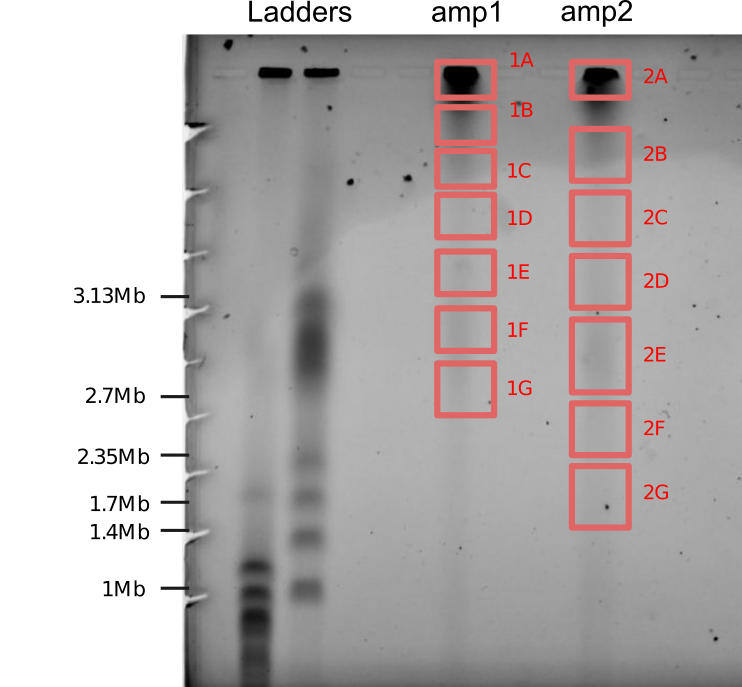
\includegraphics{cc-PFGE-gel}
        \caption{}
        \label{subfig:cc-pfge-gel}
    \end{subfigure}
    \begin{subfigure}{0.49\textwidth}
        \centering
        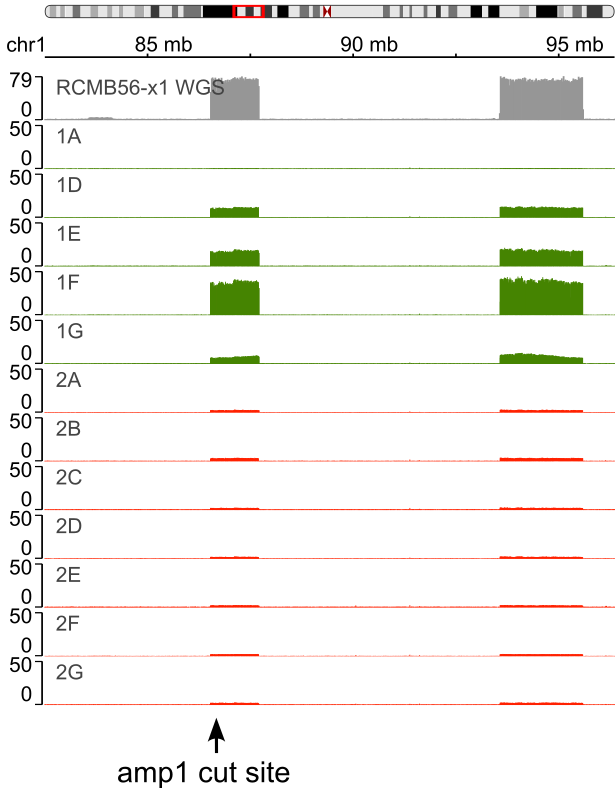
\includegraphics{cc-amp1-igv}
        \caption{}
        \label{subfig:cc-amp1-igv}
    \end{subfigure}
    \begin{subfigure}{0.44\textwidth}
        \centering
        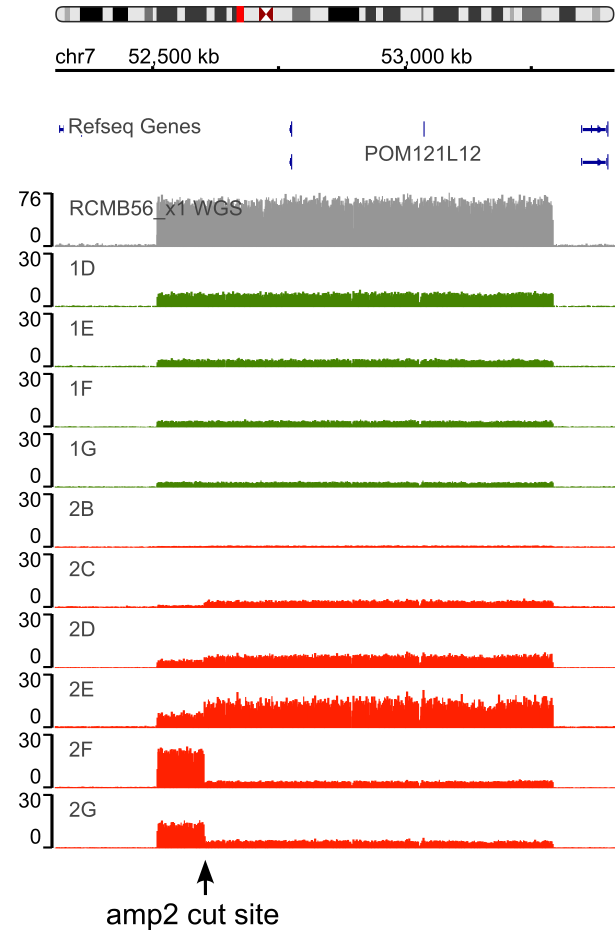
\includegraphics{cc-amp2-igv}
        \caption{}
        \label{subfig:cc-amp2-igv}
    \end{subfigure}
    \begin{subfigure}{0.54\textwidth}
        \centering
        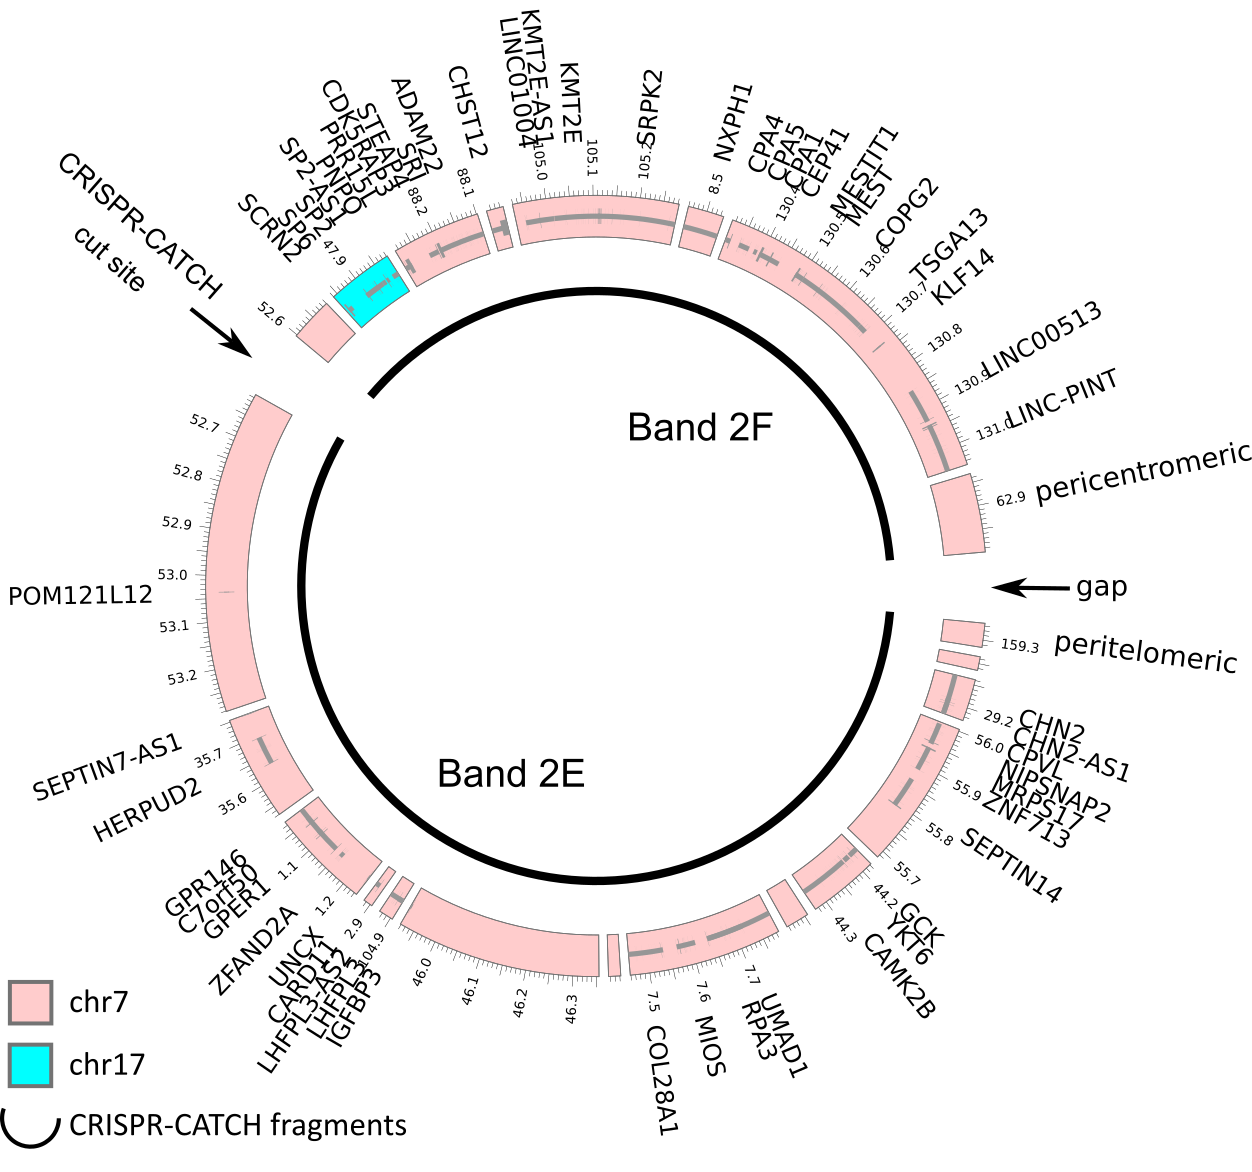
\includegraphics{cc-amp2-circos-map}
        \caption{}
        \label{subfig:cc-amp2-circos-map}
    \end{subfigure}
    \caption[CRISPR-CATCH indicates circular and linear extrachromosomal amplifications in RCMB56 tumors.]{\textbf{CRISPR-CATCH indicates circular and linear extrachromosomal amplifications in RCMB56 tumors.} (\textbf{a}) \gls{uhmw dna} from RCMB56-pdx was cut using CRISPR-Cas9 targeting locations on amp1 or amp2, then sorted by size using \gls{pfge}. Size-sorted bands were then sequenced and aligned to the human reference genome hg38. Circular and chromosomal DNA do not migrate, and are sampled in bands 1A and 1B. (\textbf{b}) \gls{wgs} depth of sequencing coverage of all bands at the amp1 locus. When amp1 is cut (green tracks), \gls{pfge} enriches linear \gls{uhmw dna} mapping to amp1 with a unimodal size distribution centered at $s \approx 3$Mbp (band 1F). When amp1 is not cut (red tracks), no enrichment of amp1 sequences is detected. (\textbf{c}) \gls{wgs} sequencing coverage of all bands at the amp2 locus. When amp2 is not cut (green tracks), \gls{pfge} enriches linear \gls{uhmw dna} mapping to amp2 with size $s \gg 3$Mbp (band 1D). When amp2 is cut (red tracks), \gls{pfge} enriches two distinct fractions of \gls{uhmw dna}, mapping to mutually exclusive fragments of the amp2  assembly and with lengths $s_1 \approx 2.8$Mbp (band 2E) and $s_2 \approx 2.4$Mbp (band 2F). (\textbf{d}) Genomic map of the fragments of amp2 enriched in bands 2E and 2F.}
    \label{fig:cc}
\end{figure}

Visual inspection of the \acrshort{wgs} data also revealed a low-copy gain (gain1) of unknown architecture composed of other segments of chr7 (35Mbp) and chr17 (800kbp). DNA \gls{FISH} imaging of metaphase cells for marker genes \textit{DNTTIP2} (amp1), \textit{KMT2E} (amp2) and \textit{ETV1} (gain1) indicated that amp1 and amp2 are amplified extrachromosomally (Fig. \ref{fig:fish-rcmb56-pdx-metaphase}). To confirm co-occurrence in the same cells, we performed multi-channel FISH imaging for the same markers in interphase cells. We observed distinct fluorescence spots for each gene, indicating that copies of each amplified gene are located on distinct chromatin bodies (Fig. \ref{fig:fish-rcmb56-ht-interphase}). 

\begin{figure}[!h]
    \centering
    \begin{subfigure}{0.32\textwidth}
        \centering
        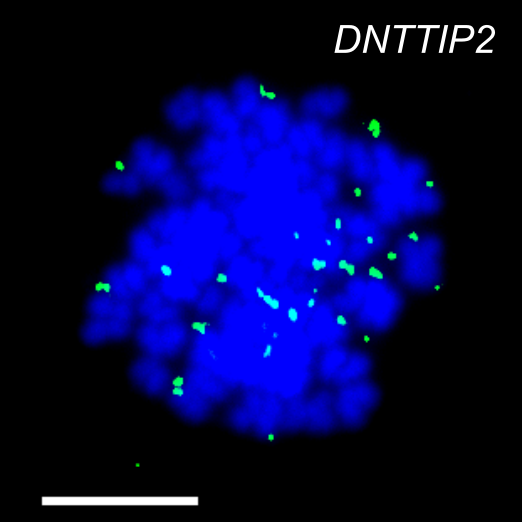
\includegraphics{rcmb56-pdx-dnttip2}
        \caption{}
        \label{subfig:}
    \end{subfigure}
    \begin{subfigure}{0.32\textwidth}
        \centering
        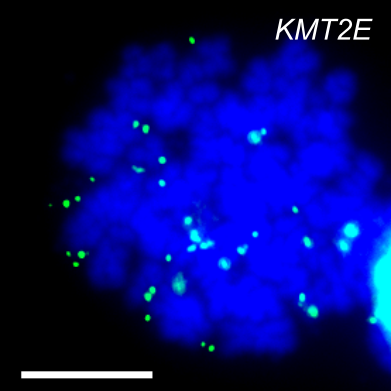
\includegraphics{rcmb56-pdx-kmt2e}
        \caption{}
        \label{subfig:}
    \end{subfigure}
    \begin{subfigure}{0.32\textwidth}
        \centering
        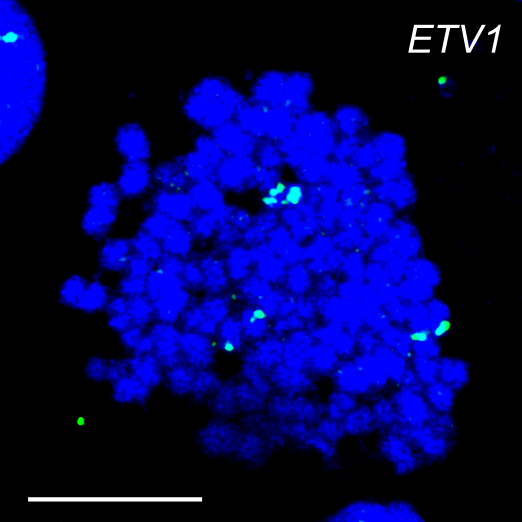
\includegraphics{rcmb56-pdx-etv1}
        \caption{}
        \label{subfig:}
    \end{subfigure}    
    \caption[FISH imaging of amplified marker genes in RCMB56-pdx metaphase cells.]{\textbf{FISH imaging of amplified marker genes in metaphase spreads of RCMB56-pdx nuclei.} (\textbf{a}) Marker gene \textit{DNTTIP2} (amp1). (\textbf{b}) Marker gene \textit{KMT2E} (amp2). (\textbf{c}) Marker gene \textit{ETV1} (gain1). DAPI chromatin stain in blue. Scale bars $10\mu$m.
    }
    \label{fig:fish-rcmb56-pdx-metaphase}
\end{figure}

\begin{figure}
    \centering
    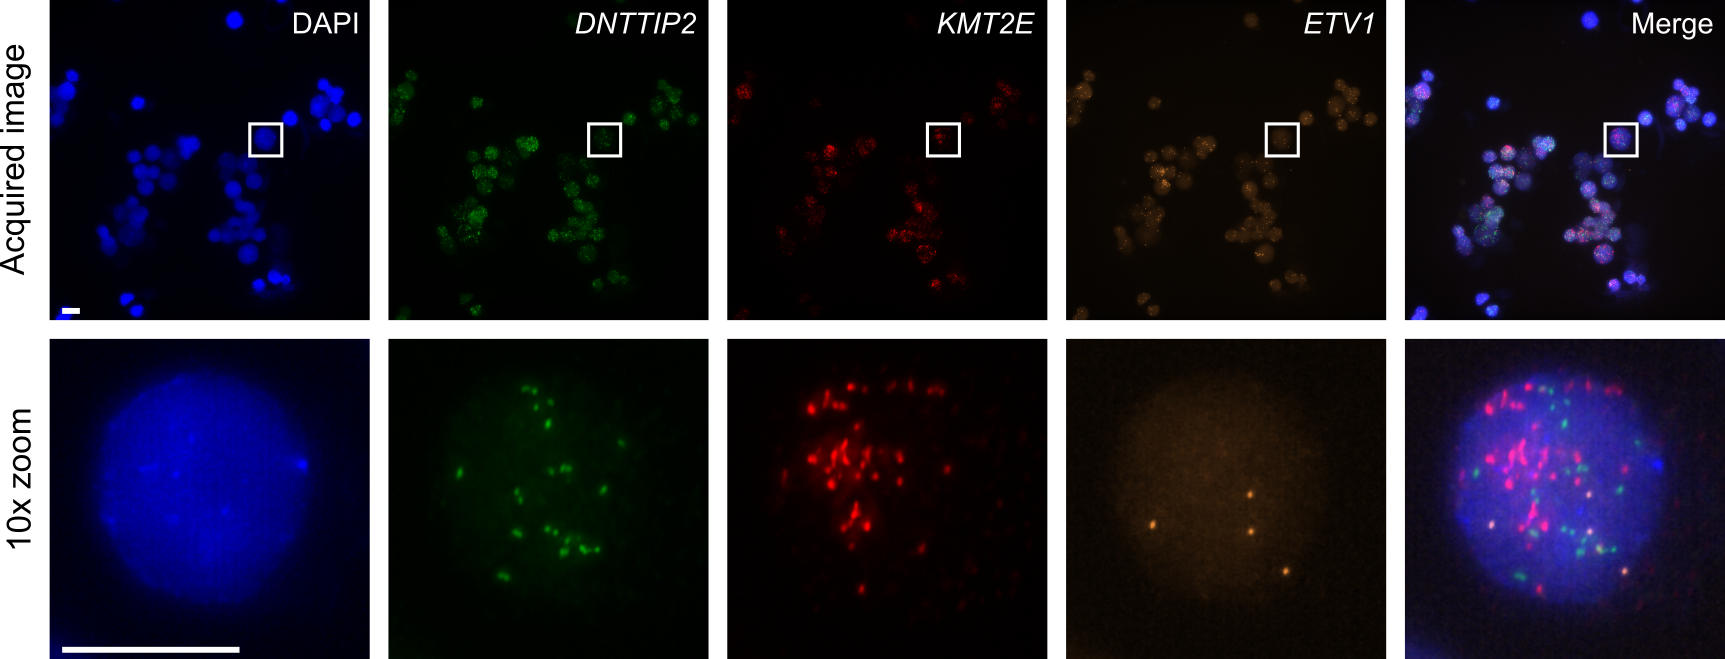
\includegraphics{rcmb56-ht-tricolor}
    \caption[Multi-channel FISH imaging of amplified marker genes in RCMB56-ht interphase cells.]{\textbf{Multi-channel FISH imaging of amplified marker genes in RCMB56-ht interphase cells.} Example image shown on top row, 10x zoom of an example single cell on bottom row. Columns from left to right: DAPI channel (chromatin), \textit{DNTTIP2} (amp1), \textit{KMT2E} (amp2), \textit{ETV1} (gain1), merge of all channels. Marker gene copies are spatially independent, indicating distinct amplifications of all 3 markers in the same cells. 
    }
    \label{fig:fish-rcmb56-ht-interphase}
\end{figure}

\subsection{MB patient tumors with ecDNA exhibit high intratumoral copy number heterogeneity.}
Substantial intratumoral copy number heterogeneity is expected in an ecDNA+ tumor due to random segregation of ecDNA during mitosis, driving tumor evolution and treatment resistance \cite{Lange_2021}.  To determine the extent of ecDNA copy number heterogeneity in patient MB tumors, we established an automated image analysis pipeline to estimate the distributions of copy number per cell in interphase FISH microscopy imaging (see Methods \ref{methods:fish}) and applied it to four primary MB tumors harboring ecDNA: MB036 (\textit{MYCN}), MB177 (\textit{MYCN}), MB268 (\textit{MDM4}), and RCMB56 (\textit{DNTTIP2}, \textit{KMT2E}, \textit{ETV1}). The estimated copy number per cell of all ecDNA-amplified marker genes had significantly greater mean (Wilcoxon test) and variance (Levene's test) than the ecDNA- cell line COLO320-HSR (Fig. \ref{fig:fish-heterogeneity}) which includes \textit{MYC} on a chromosomal amplification \cite{hung_2021}. These results from human MB tumors are consistent with high copy number heterogeneity observed in human cancer cell lines with ecDNA \cite{Lange_2021}. In each primary tumor analyzed, ecDNA was amplified (copy number greater than 5) in only a subset of cells (22-41\%, Supplementary Table 5 of \cite{Chapman}). 

\begin{figure}[!h]
    \centering
    \centerline{%
    \begin{subfigure}{1.1\textwidth}
        \centering
        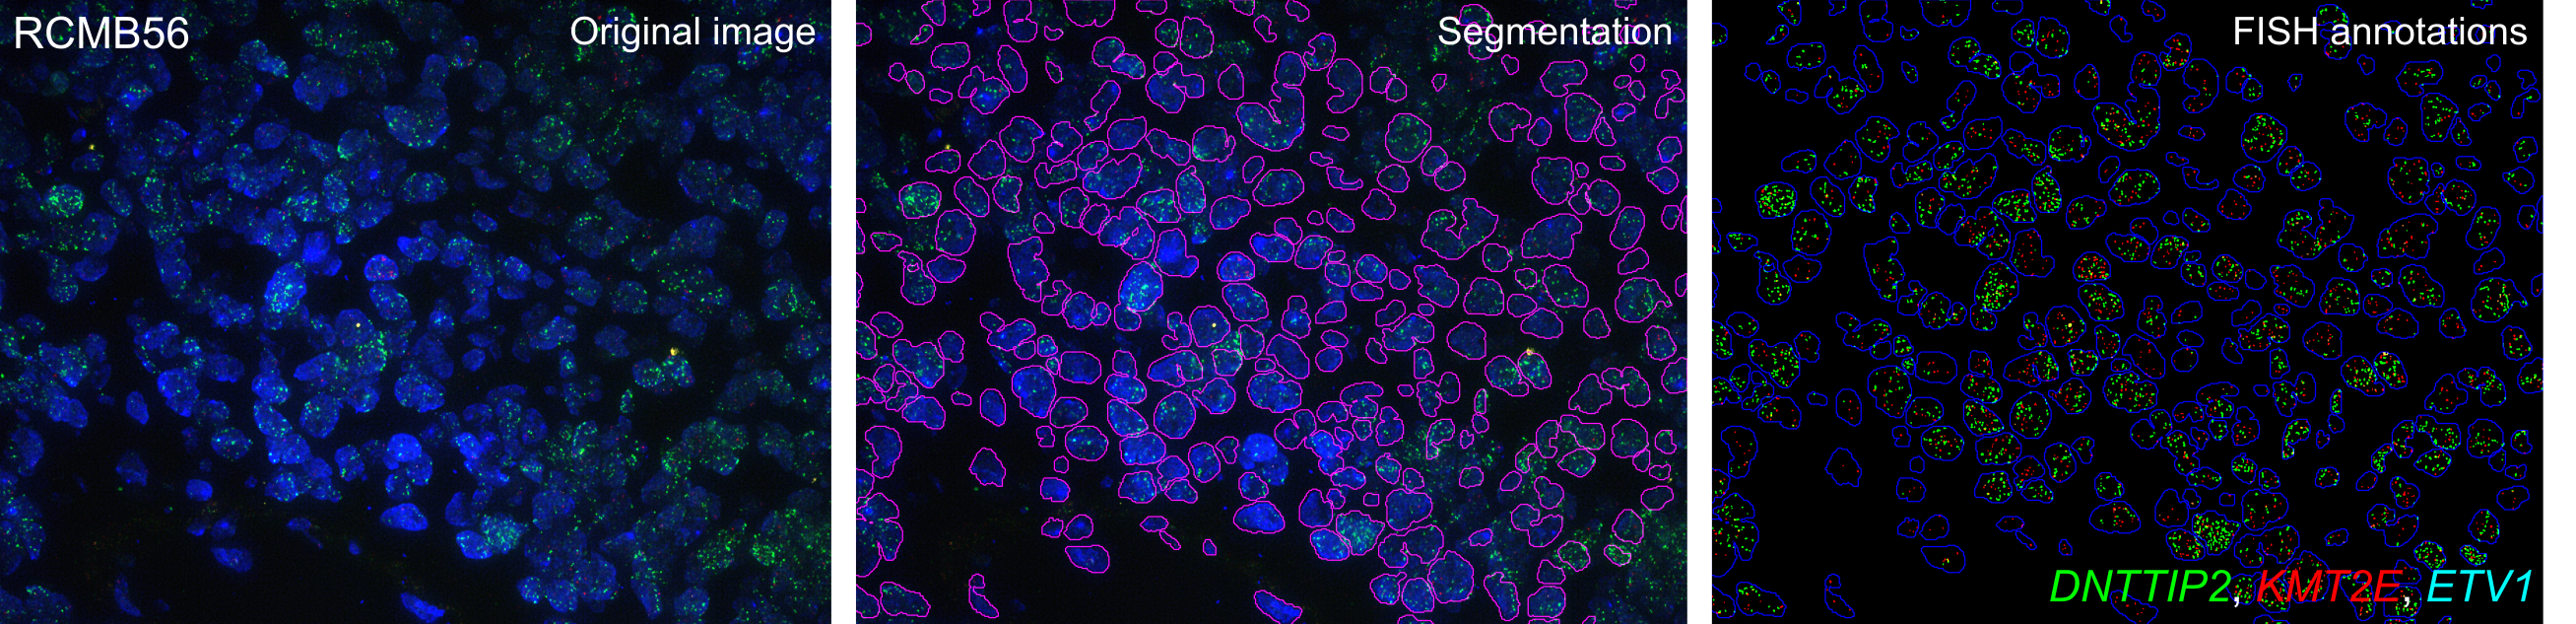
\includegraphics{rcmb56-ht-segmentation}
        \caption{}
        \label{subfig:fish-segmentation}
    \end{subfigure}%
    }
    \centerline{%
    \begin{subfigure}{1.1\textwidth}
        \centering
        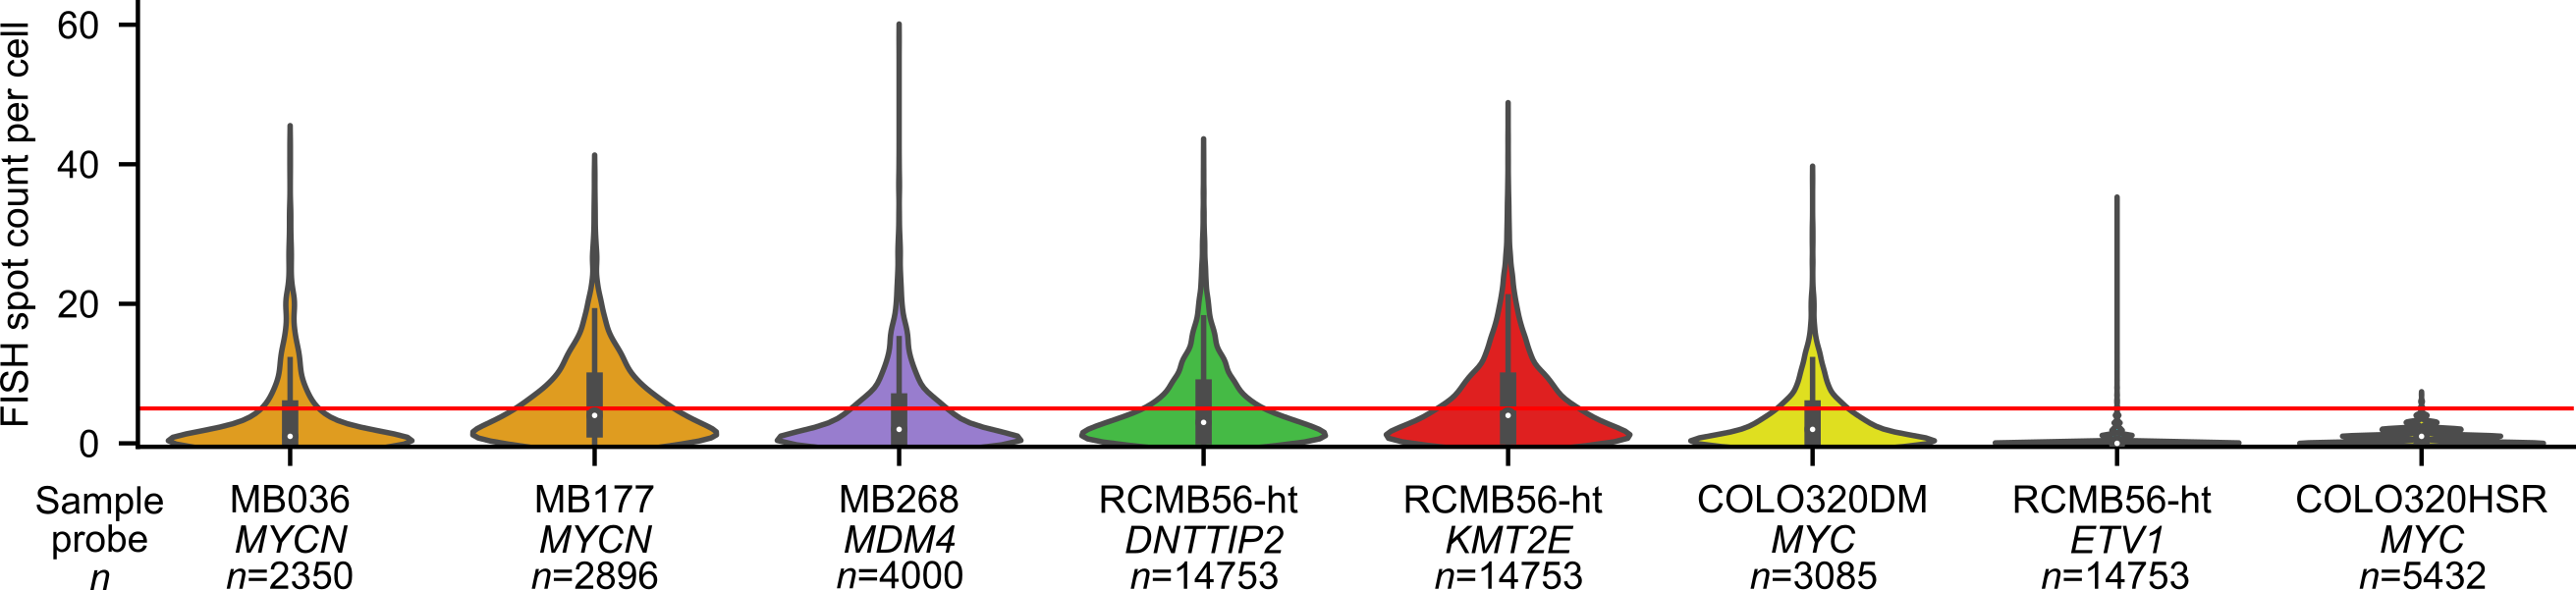
\includegraphics{violin-fish-counts}
        \caption{}
        \label{subfig:violin-fish-counts}
    \end{subfigure}%
    }
    \caption[Copy number estimation of ecDNA in single cells from FISH microscopy]{\textbf{Copy number estimation of ecDNA in single cells from FISH microscopy.} (\textbf{a}) Example output of automated image analysis pipeline. Segmentation: nuclear boundaries were detected from the DAPI channel image using NuSeT \cite{nuset}. FISH annotations: The number of FISH foci was inferred using ecSeg-i \cite{ecseg}. (\textbf{b}) Estimated copy counts for amplified foci on ecDNA and other copy gains. Red line indicates $n\geq5$, the threshold whereupon a cell was classified as amplified.
    }
    \label{fig:fish-heterogeneity}
\end{figure}

\par To determine whether copy number heterogeneity of an ecDNA+ tumor is accompanied by transcriptional heterogeneity, we analyzed 2,762 single nuclei from frozen tissue of RCMB56-ht using a multiome snRNA+ATAC-seq assay (10X Genomics) to profile transcriptomes and accessible chromatin of the same individual cells. Consistent with previous findings in bulk samples \cite{Turner_2017,Wu_2019} RCMB56-ht single nucleus ATAC-seq (snATAC-seq) sequencing coverage was enriched at the amp1 and amp2 loci at the aggregate level, and also in individual cells (Fig. \ref{subfig:scATAC-coverage}). To detect focal amplifications in single nuclei, we performed Monte Carlo permutation tests comparing snATAC-seq read density at the amplicon locus to that at random locations elsewhere in the genome (excluding blacklisted regions, see Methods \ref{methods:ssgsea}). Z-score normalized read density at the amp1 and amp2 loci had greater mean and variance than at gain1 (Fig. \ref{subfig:violin-scatac-coverage}), consistent with the copy number heterogeneity we observed in the interphase FISH data. We conservatively estimate that at least 224 out of 2762 (8\%, FDR $q < 0.10$) cells contained amp1 or amp2 (ecDNA+ cells). Of these, both amp1 and amp2 were detected together in only a minority of cells (72 out of 224, 32\%) (Fig. \ref{subfig:venn-ecDNA+cells}). Thus, evidence from quantitative FISH microscopy and multiome single-cell sequencing show that only a fraction of tumor cells in ecDNA+ MB tumors harbor high-copy ecDNA, and that these have highly variable copy numbers of extrachromosomal amplifications. 

\begin{figure}[!h]
    \centering
    \centerline{%
    \begin{subfigure}{1.2\textwidth}
        \centering
        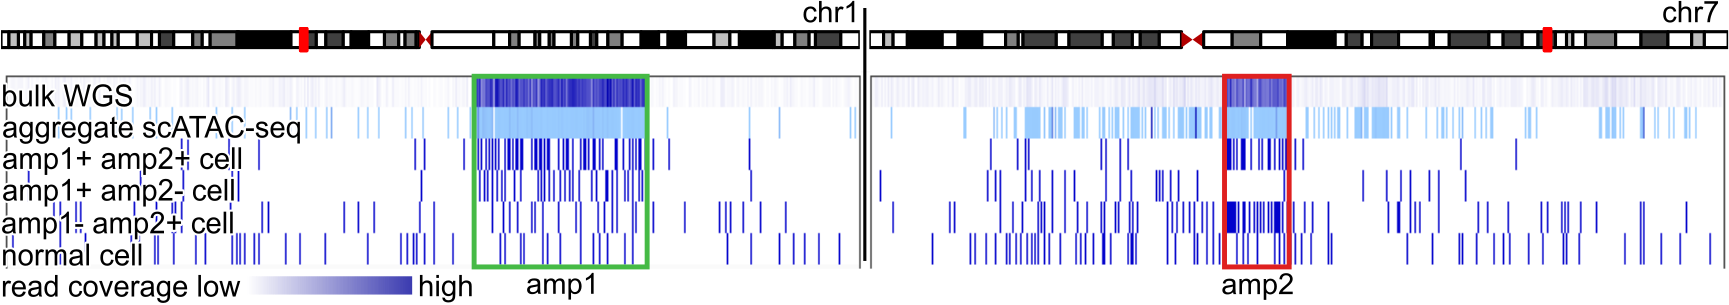
\includegraphics{scATAC-coverage}
        \caption{}
        \label{subfig:scATAC-coverage}
    \end{subfigure}%
    }
    \begin{subfigure}{.49\textwidth}
        \centering
        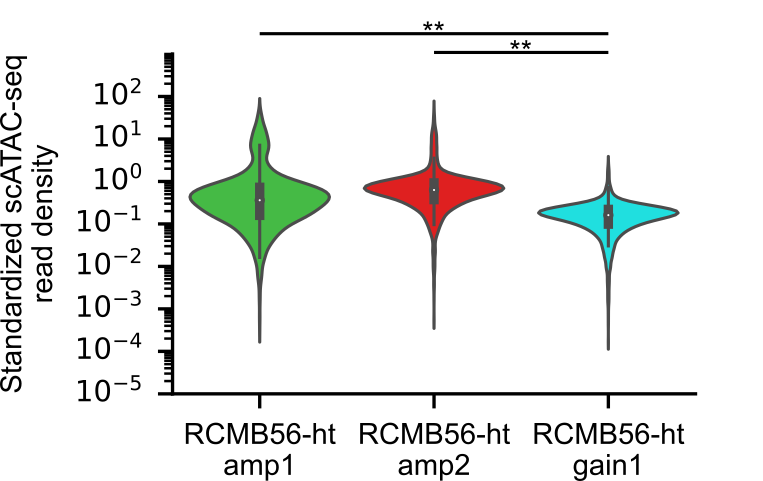
\includegraphics{scATAC-coverage-violin}
        \caption{}
        \label{subfig:violin-scatac-coverage}
    \end{subfigure}
    \begin{subfigure}{.49\textwidth}
        \centering
        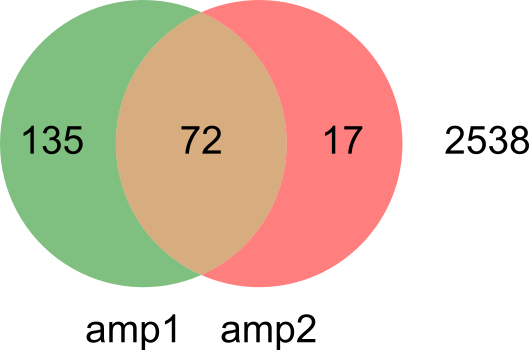
\includegraphics{rcmb56-ht-ecDNA+classifications}
        \caption{}
        \label{subfig:venn-ecDNA+cells}
    \end{subfigure}
    \caption[Detection of ecDNA in in single cells from single-cell ATAC-seq of RCMB56-ht.]{\textbf{Detection of ecDNA in in single cells from single-cell ATAC-seq of RCMB56-ht.} (\textbf{a}) Mapped read density of sequencing modalities at RCMB56 amp1 and amp2 loci. Tracks from top to bottom: bulk \gls{wgs}, aggregate scATAC-seq across all cells, and scATAC-seq of individual cells. (\textbf{b}) Distribution of Z-score normalized read coverage at the amp1, amp2, and gain1 loci. ** $p < 0.005$, Mann-Whitney test. (\textbf{c}) Sets of RCMB56 cells identified as harboring high-copy amplification of amp1 and amp2. Monte Carlo permutation test, $q < 0.05$.
    }
    \label{fig:scatac-heterogeneity}
\end{figure}

\subsection{ecDNA+ and ecDNA- tumor cell populations in the same tumor have distinct transcriptional profiles.}
Clustering single cells using the Weighted Nearest Neighbors algorithm (WNN, \cite{seurat_4}) placed the majority of ecDNA+ cells in a single cluster with distinct transcriptional and epigenetic features (Fig. \ref{fig:rcmb56-ht-clustering}). As expected, cells in the ecDNA+ cluster overexpressed \textit{DNTTIP2} ($q < 0.001$, Wilcoxon Rank Sum test) and \textit{KMT2E} ($q < 0.001$), the marker genes amplified on amp1 and amp2. Compared with other tumor and normal cells, ecDNA+ tumor cells also overexpressed \textit{GLI2} ($q < 0.001$), a known mediator of SHH-mediated transcription and a marker for SHH \gls{MB}, despite \textit{GLI2} not being affected by copy number alteration in this tumor. (Fig. \ref{subfig:clustering-exp-dotplot}, Supplementary Table 6 of \cite{Chapman}). To further investigate the relationship between ecDNA copy number and transcription, we estimated first, ecDNA copy number in single cells (z-scores), and second, the transcriptional activity of genes amplified on ecDNA in each cell (ssGSEA \cite{ssGSEA_2009} scores, see Methods \ref{methods:ssgsea}). As expected, ssGSEA scores were positively correlated with z-scores, indicating increased transcription of ecDNA-amplified genes with increasing ecDNA copy number (Fig. \ref{fig:ssgsea-x-zscores}). 

\begin{figure}[!h]
    \centering
    \begin{subfigure}{.49\textwidth}
        \centering
        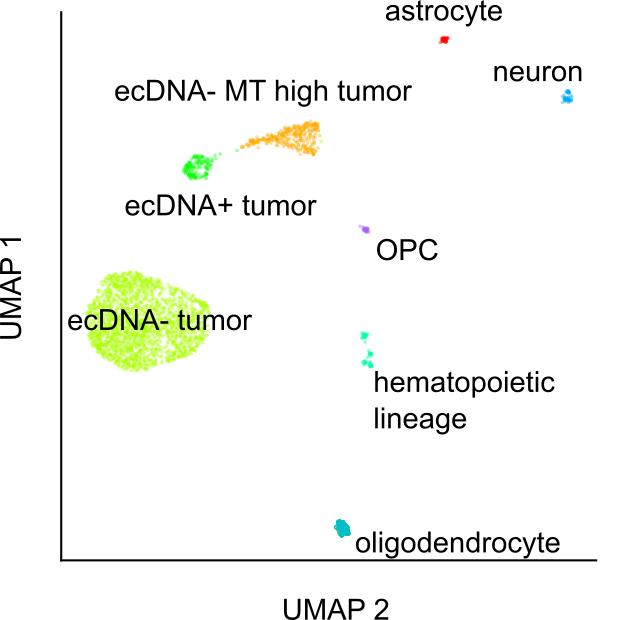
\includegraphics{rcmb56-ht-celltype-umap-v2}
        \caption{}
        \label{subfig:clustering-celltypes}
    \end{subfigure}
    \begin{subfigure}{.49\textwidth}
        \centering
        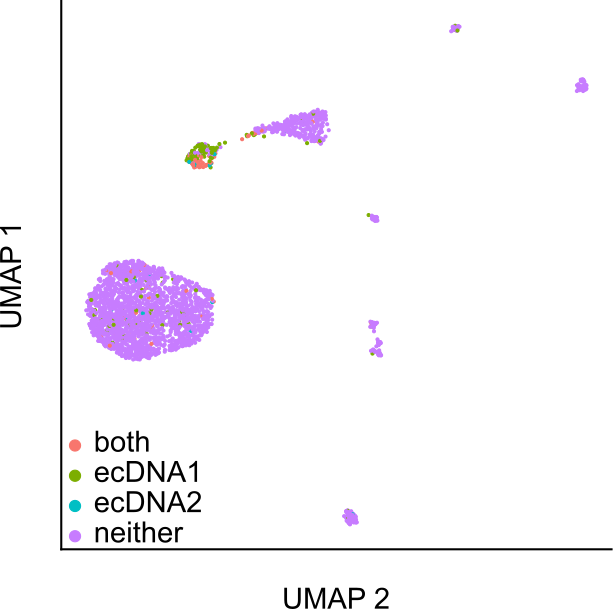
\includegraphics{rcmb56-ht-ecDNA-status-umap}
        \caption{}
        \label{subfig:clustering-ecDNA-status}
    \end{subfigure}
    \begin{subfigure}{.49\textwidth}
        \centering
        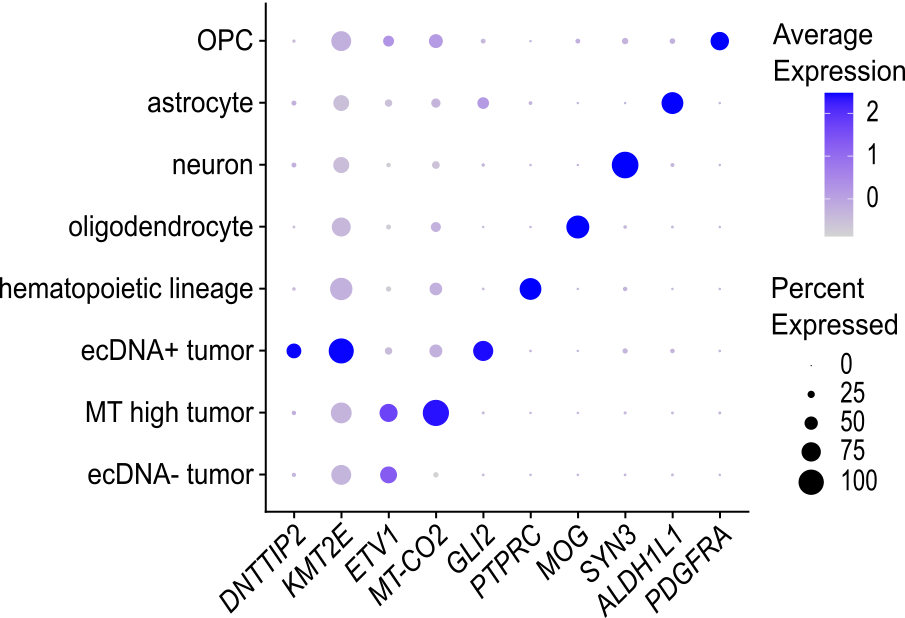
\includegraphics{rcmb56-ht-dotplot}
        \caption{}
        \label{subfig:clustering-exp-dotplot}
    \end{subfigure}
    \caption[RCMB56 ecDNA+ cells express a distinct transcriptional and epigenetic profile.]{\textbf{RCMB56 ecDNA+ cells express a distinct transcriptional and epigenetic profile.} (\textbf{a}) UMAP projection of 2,762 RCMB56-ht cells were clustered by joint transcriptional and epigenetic profiles using the WNN algorithm \cite{seurat_4}. ecDNA- tumor: cells harboring other structural variants but not enriched for ecDNA (see also Fig. \ref{fig:rcmb56-ht-infercnv}). ecDNA- MT high: ecDNA- tumor cells with high expression of mitochondiral genes. Normal cells were identified by expression of marker genes. (\textbf{b}) UMAP projection of RCMB56-ht cells labelled by high-copy focal amplification of ecDNA, identifed by depth of scATAC-seq coverage at ecDNA loci. (\textbf{c}) Transcription of marker genes in single cells of RCMB56-ht.  
    }
    \label{fig:rcmb56-ht-clustering}
\end{figure}

\begin{figure}[!h]
    \centering
    \begin{subfigure}{.49\textwidth}
        \centering
        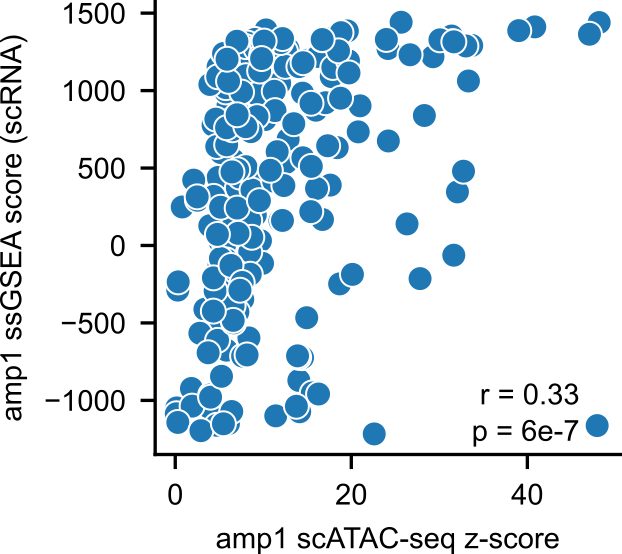
\includegraphics{ssgsea1-x-zscore1}
        \caption{}
    \end{subfigure}
    \begin{subfigure}{.49\textwidth}
        \centering
        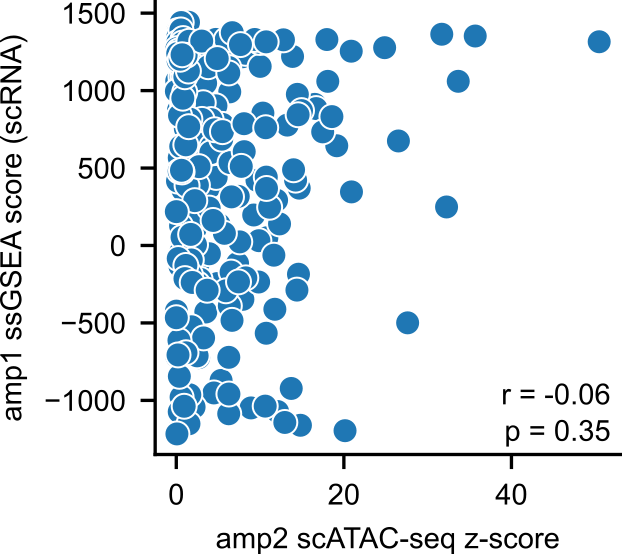
\includegraphics{ssgsea1-x-zscore2}
        \caption{}
    \end{subfigure}
    \begin{subfigure}{.49\textwidth}
        \centering
        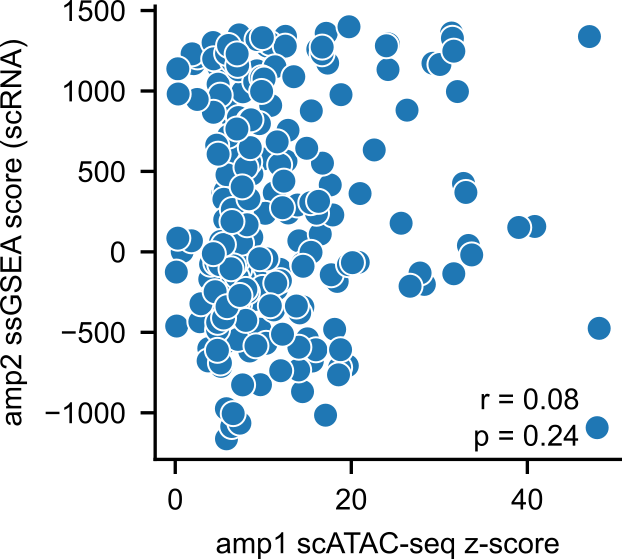
\includegraphics{ssgsea2-x-zscore1}
        \caption{}
    \end{subfigure}
    \begin{subfigure}{.49\textwidth}
        \centering
        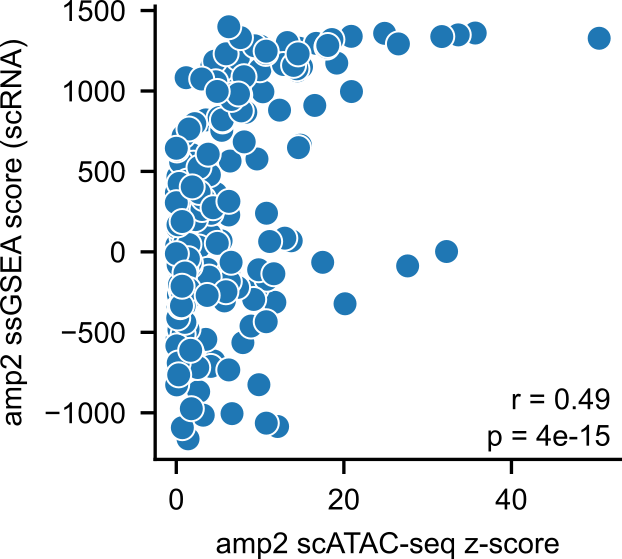
\includegraphics{ssgsea2-x-zscore2}
        \caption{}
    \end{subfigure}
    \caption[ecDNA copy number is associated with gene expression of ecDNA-amplified genes.]{\textbf{ecDNA copy number is associated with gene expression of ecDNA-amplified genes.} Pearson correlations between copy number at the amplified locus (z-scores) and transcriptional activity of amplified genes (ssGSEA scores). Copy number of amp1 is associated with transcription of amp1-amplified genes, but not with transcription for amp2-amplified genes. Conversely, copy number of amp2 is associated with amp2-amplified, but not amp1-amplified, gene expression. 
    }
    \label{fig:ssgsea-x-zscores}
\end{figure}

In addition to the ecDNA+ tumor cells, we identified two other clusters of tumor cells not enriched for ecDNA and with low expression of the amp1 and amp2 marker genes, one of which strongly expressed mitochondrial genes (`ecDNA-' and `ecDNA- MT high'), as well as normal cells such as astrocytes, oligodendrocytes and cells from the hematopoietic lineage (Fig. \ref{subfig:clustering-exp-dotplot}). Normal cell types were annotated by cell cluster-specific expression of known marker genes. Genomic copy number estimation from snRNA-seq confirms that normal cells had stable genomes whereas the tumor cells were characterized by copy-number alterations (Fig. \ref{fig:rcmb56-ht-infercnv}). 

\begin{figure}[!h]
    \centering
    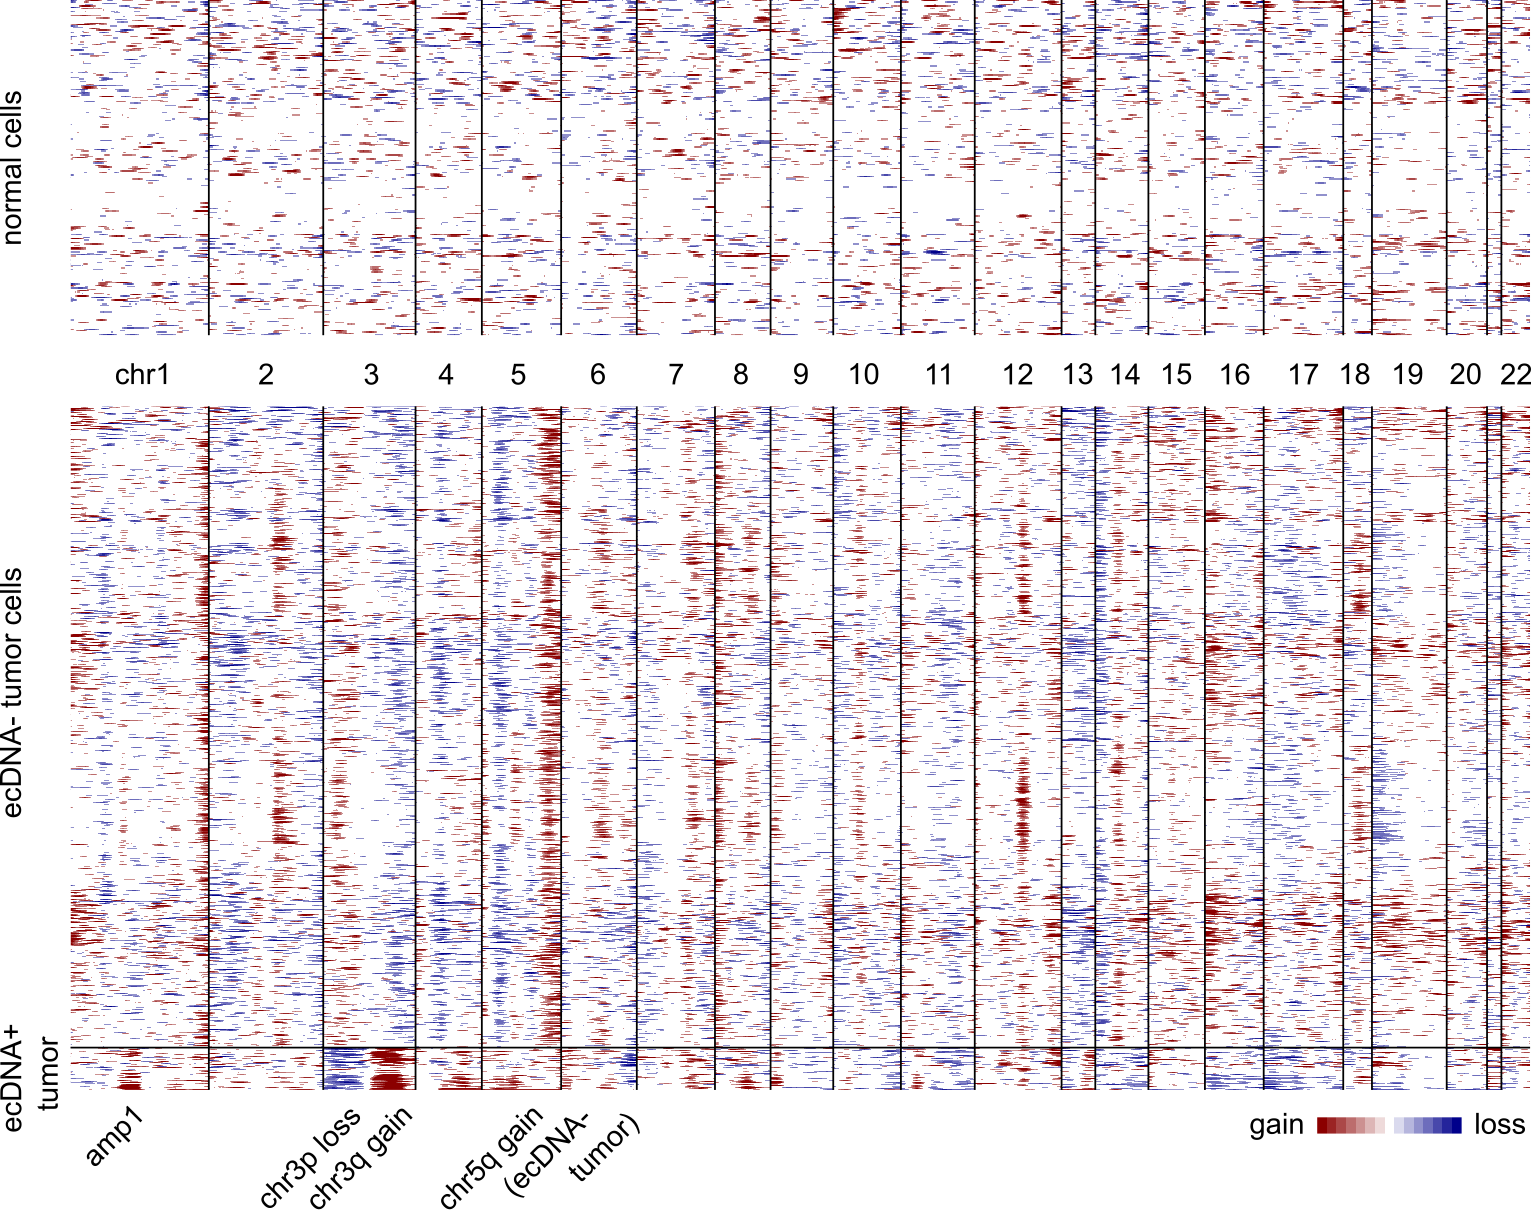
\includegraphics{rcmb56-ht-infercnv}
    \caption[Aneuploidy estimated from single-cell transcriptomes of 2,762 cells from RCMB56-ht]{\textbf{Aneuploidy estimated from single-cell transcriptomes of 2,762 cells from RCMB56-ht} using inferCNV \cite{inferCNV_2019}. Diploid cells comprising the astrocyte, neuron, OPC, hematopoietic and oligodendrocyte cell clusters comprised the reference set of normal cells. The cluster enriched for high-copy ecDNA is annotated. This cluster also uniquely harbors chr3p deletion and chr3q gain.}
    \label{fig:rcmb56-ht-infercnv}
\end{figure}

\subsection{A PDX model resembles ecDNA+ cells of its origin human tumor.}

Patient-derived xenografts (PDX) and cell lines have been used as preclinical models for identification and testing of compounds for new targeted therapies for MB \cite{rusert_2020}. To test whether cells in a PDX faithfully model ecDNA in the corresponding human tumor, we applied multiome scRNA+ATAC-seq to fresh tissue from passage 1 of the RCMB56-pdx model. In contrast to RCMB56-ht, nearly every human cell in the RCMB56-pdx sample contained ecDNA (9608 out of 9,620, 99.96\%, $q < 0.10$) (Fig. 4f, Supplementary Fig. 7b). The majority of these contained both amp1 and amp2 (8554 out of 9608, 89\%). Batch-correction and dimensionality reduction on the unified set of transcriptomes from both samples, using the Conos package \cite{conos_2019}, indicates that the cells of the PDX are transcriptionally similar to ecDNA+ cells in RCMB56-ht, and distinct from all other RCMB56-ht cells (Fig. \ref{fig:rcmb56-pdx-clustering}). We then asked whether the human tumor ecDNA+ cell subpopulation harbored additional identifying genomic alterations which could be confirmed in the PDX. Genomic copy number estimation from the scRNA-seq data indicated that tumor cells of the RCMB56-ht ecDNA+ cluster uniquely harbored chr3p deletion and chr3q duplication but not chr5q duplication (Fig. \ref{fig:rcmb56-ht-infercnv}). Cells from RCMB56-pdx universally harbored the same alterations (Fig. \ref{fig:rcmb56-pdx-infercnv}). These results indicate that the PDX tumor RCMB56-pdx is a clonal expansion of the ecDNA+ cells of the human tumor RCMB56-ht. 

\begin{figure}[!h]
    \centering
    \begin{subfigure}{.49\textwidth}
        \centering
        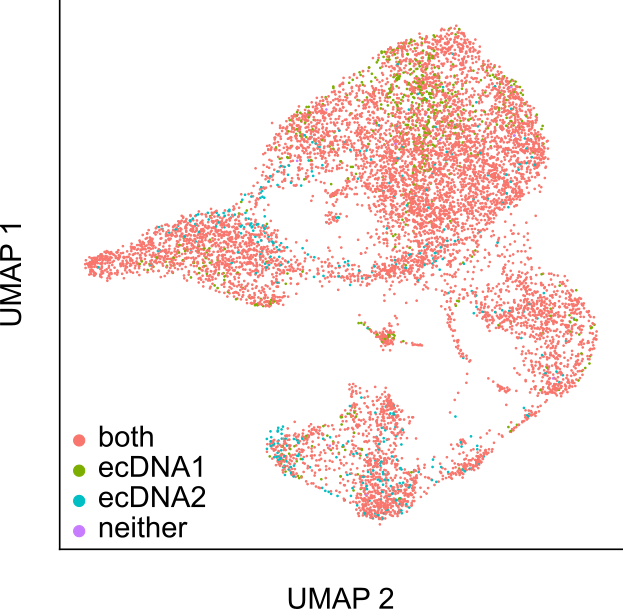
\includegraphics{rcmb56-pdx-ecDNA-status-umap}
        \caption{}
    \end{subfigure}
    \begin{subfigure}{.49\textwidth}
        \centering
        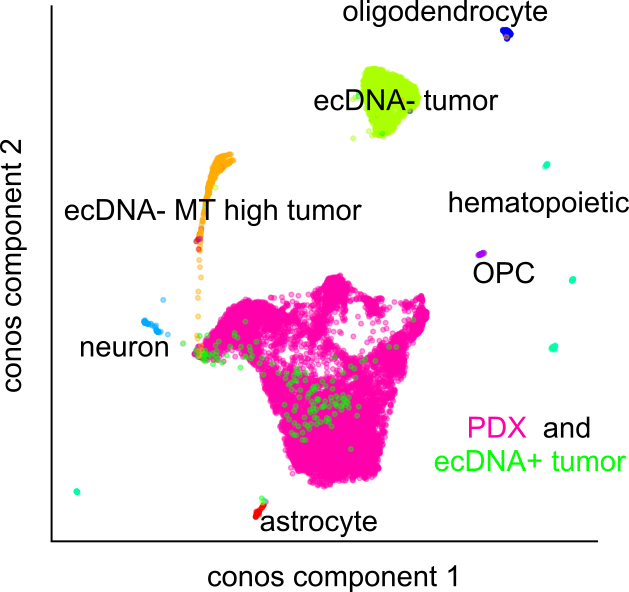
\includegraphics{rcmb56-pdx-conos}
        \caption{}
        \label{subfig:conos}
    \end{subfigure}
    \caption[High-copy ecDNA is universally present in 9,620 RCMB56-pdx cells.]{\textbf{High-copy ecDNA is universally present in 9,620 RCMB56-pdx cells.} (\textbf{a}) Low-dimensional UMAP embedding of 9,620 RCMB56-pdx accessible chromatin and transcriptomes, annotated by ecDNA detected by scATAC-seq. (\textbf{b}) Low-dimensional embedding of 9,620 RCMB56-pdx and 2,762 RCMB56-ht transcriptomes, integrated and batch-corrected using Conos \cite{conos_2019}. PDX cells (pink) overlap ecDNA+ cells from the patient tumor, but are distinct from other RCMB56-ht cell clusters.}
    \label{fig:rcmb56-pdx-clustering}
\end{figure}

\begin{figure}[!h]
    \centering
    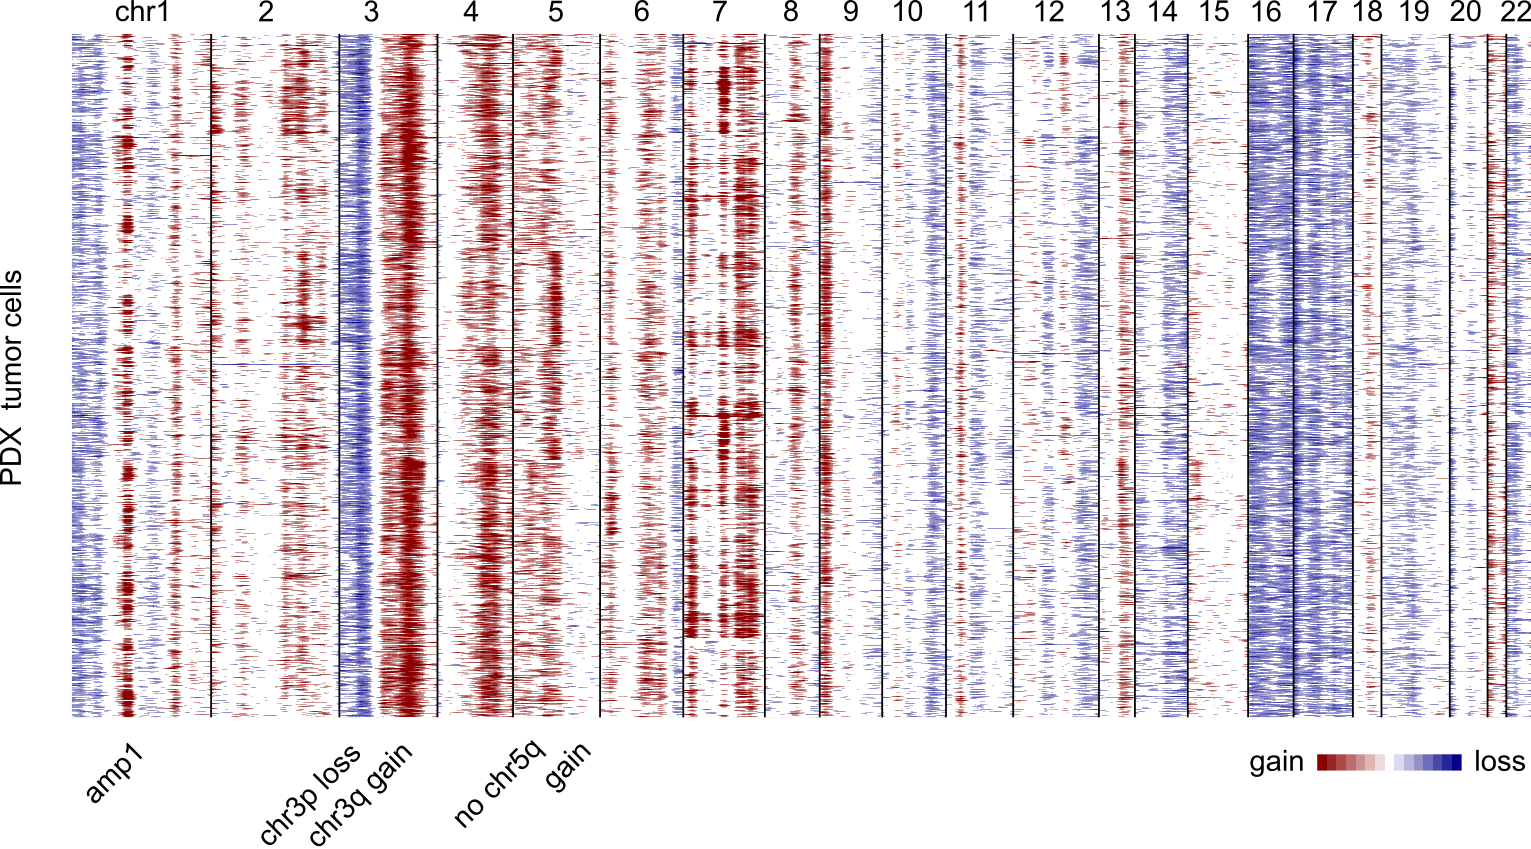
\includegraphics{rcmb56-pdx-infercnv}
    \caption[Aneuploidy estimated from single-cell transcriptomes of 9,620 cells from RCMB56-pdx]{\textbf{Aneuploidy estimated from single-cell transcriptomes of 9,620 cells from RCMB56-pdx} using inferCNV \cite{inferCNV_2019}. PDX cells univerally harbor the chromosomal copy gain (chr3q) and loss (chr3p) which uniquely identify ecDNA+ cells in the RCMB56-ht human tumor (Fig. \ref{fig:rcmb56-ht-infercnv}).
    }
    \label{fig:rcmb56-pdx-infercnv}
\end{figure}

\subsection{The relapsed RCMB56 patient tumor karyotype was present in a subpopulation of ecDNA+ cells in the primary.}
Following maximal resection, the RCMB56 primary tumor had been treated according to the standard of care with high-dose craniospinal proton therapy and chemotherapy including cisplatin, cyclophosphamide, and vincristine \cite{rusert_2020}. Two years after initial diagnosis, however, the RCMB56 tumor recurred and a second surgical resection was performed. WGS data from \gls{FFPE} tissue of the relapsed tumor (RCMB56-r1) indicated copy-number amplification at the amp1 locus but not the amp2 locus (data not shown). Computational reconstruction using \gls{AA} confirmed that the amp1 sequence remained largely unchanged. Following WGS, no tissue remained of the relapsed tumor for further analysis. Thus, although we cannot rule out that amp2 was present in an area of the relapsed tumor which was not sampled, we observe amp1 but no evidence of amp2 in the RCMB56 relapsed patient tumor.

\section{Discussion}
Analyses of the p53-mutant SHH tumor RCMB56-ht reveal intratumoral heterogeneity not present in subsequent longitudinal biopsies of the same tumor. Sequence assembly, from whole genome short-read sequencing, optical genome mapping on long reads, and CRISPR-CATCH, reconstructs two distinct high-copy extrachromosomal focal amplifications, one from 3 segments of chr1 and the other from 20 segments of chr7 and chr17. Analyses of FISH microscopy and single-cell sequencing of RCBM56-ht tissue concur that both amplicons may be found in the same tumor cells, and that amplicon copy number is highly variable between cells. Further analysis of multi-omic single-cell sequencing data reveals that tumor cells with high-copy ecDNA expressed a distinct transcriptional and epigenetic program, including \textit{GLI2}, a marker of malignant SHH subgroup MB. Thus, the RCMB56 patient tumor comprised a population of cells with heterogeneous ecDNA sequences, ecDNA copy number, and cell states. 

\par Although ecDNA+ and ecDNA- tumor cells coexisted in RCMB56-ht, the presence or absence of ecDNA became fixed in subsequent tumors descended from the primary tumor. In the relapsed tumor RCMB56-r1, resected 2 years after original diagnosis, we find amp1 but no evidence of amp2. In RCMB56-pdx, amp1 and amp2 are near-univerally present, indicating loss of the ecDNA- tumor cell subpopulation during engraftment. Thus, in either RCMB56 tumor, we observe substantial changes of intratumoral heterogeneity of ecDNA following a strong selective pressure. It remains to be seen whether similar changes in ecDNA+ cell populations occur in other patient tumors during tumor progression, or in other PDX models under selective pressure.

\par Data from multiple modalities confirm the circular extrachromosomal sequence of amp1, but not amp2. Whereas sequence assembly from \gls{wgs} and \gls{ogm} data fully reconstruct the circular amp1 sequence, the same data map a linear amp2 sequence assembly, with ends mapping to pericentromeric and peritelomeric regions of chr7. Cutting circular amp1 by CRISPR-CATCH yields linear DNA of the approximate length of the amp1 assembly, but cutting amp2 results in 2 fractions of linear DNA, whose lengths and sequences sum to the length and sequence of the amp2 assembly. In chapter 3, we will observe in Hi-C data that the ends of the amp2 assembly do not co-localize spatially. Nevertheless, amp2 appears a high-copy extrachromosomal amplification in FISH imaging, and the copy number distribution per cell resembles that of circular amp1. The base-resolution sequences of the amp2 assembly ends remain an intriguing unresolved question, and may shed light on whether stable linear extrachromosomal amplification can arise in human tumors.

% \par Short concluding comments. What is the one-sentence takeaway?

\section{Methods}
\subsubsection{Animals}
NOD-SCID IL2R$\gamma$ null (NSG) mice used for intracranial human tumor transplantation were purchased from The Jackson Laboratory (\#005557). Mice were bred and maintained in the animal facilities at the Sanford Consortium for Regenerative Medicine. All experiments were performed in accordance with national guidelines and regulations, and with the approval of the animal care and use committees at the Sanford Burnham Prebys Medical Discovery Institute and University of California San Diego (San Diego, CA, USA).

\subsubsection{Establishment and maintenance of \acrshort{rcmb56-pdx}}
The \acrlong{rcmb56-pdx} model was established by implanting 0.5-1x106 dissociated patient tumor cells directly into the cerebellum of NSG mice. Subsequent tumors were harvested from mice, dissociated and reimplanted into new NSG mice without \textit{in vitro} passaging. \textit{Ex vivo} experiments were performed with PDX RCMB56 cells of \textit{in vivo} passage 1 (x1).

\subsection{Optical genome mapping data collection and processing}
Ultra-high molecular weight (UHMW) DNA was extracted from frozen cells preserved in DMSO following the manufacturer's protocols (Bionano Genomics, USA). Cells were digested with Proteinase K and RNAse A. DNA was precipitated with isopropanol and bound with nanobind magnetic disks. Bound UHMW DNA was resuspended in the elution buffer and quantified with Qubit dsDNA assay kits (ThermoFisher Scientific).
\par DNA labeling was performed following manufacturer's protocols (Bionano Genomics, USA). Standard Direct Labeling Enzyme 1 (DLE-1) reactions were carried out using 750 ng of purified UHMW DNA. The fluorescently labeled DNA molecules were imaged sequentially across nanochannels on a Saphyr instrument. A genome coverage of at least 400x was achieved for all samples. 
\par \textit{De novo} assemblies of the samples were performed with Bionano's \textit{De Novo} assembly Pipeline (DNP) using standard haplotype aware arguments (Bionano Solve v3.6). With the Overlap-Layout-Consensus paradigm, pairwise comparison of DNA molecules was used to create a layout overlap graph, which was then used to generate the initial consensus genome maps. By realigning molecules to the genome maps ($p<10^{-12}$) and by using only the best matched molecules, a refinement step was done to refine the label positions on the genome maps and to remove chimeric joins. Next, during an extension step, the software aligned molecules to genome maps ($p<10^{-12}$), and extended the maps based on the molecules aligning past the map ends. Overlapping genome maps were then merged ($p<10^{-16}$). These extension and merge steps were repeated five times before a final refinement ($p<10^{-12}$) was applied to ``finish" all genome maps.

\subsection{ecDNA reconstruction with OGM data}
We used an ecDNA reconstruction strategy which incorporated the short-read derived CN-aware breakpoint graph generated by AA\cite{AA} with OGM contigs generated by the Bionano \textit{de novo} assembly Pipeline, and in RCMB56 we utilized contigs from both the Bionano DNP as well as the Rare Variant Pipeline (RVP).
\par We used AmpliconReconstructor (AR) v1.01\cite{AR} to scaffold together individual breakpoint graph segments using the collection of OGM contigs. We ran AR with the --noConnect flag set and otherwise default settings. A subset of informative contigs with alignments to multiple graph segments as well as a breakpoint junction were then selected for subsequent scaffolding by AR, using the ``--contig\_subset" argument of AR's OMPathFinder.py script. For exploration of unaligned regions of OGM contigs used in the reconstructions, we utilized the OGM alignment tool FaNDOM\cite{fandom} v0.2 (default settings). FaNDOM was used to identify the loose ends of the RCMB56 amp2. 
\par RCMB56 amp1 and D458 were fully reconstructed as described above; however, RCMB56 amp2 required more manual intervention. Due to the fractured nature of the breakpoint graphs in RCMB56 amp2, we searched for CN-aware paths in the AA breakpoint graph (using the plausible\_paths.py script from the AmpliconSuite pipeline), then converted these to in silico OGM sequences and aligned paths to OGM contigs directly using AR's SegAligner. 

\subsubsection{Metaphase spreads}
Cell lines were enriched for metaphases by addition of KaryoMAX (Gibco) at 0.1\textmugreek g/mL for between 2h.-overnight (0.02\textmugreek g/mL overnight for dissociated PDX cells). Single cell suspensions were then incubated with 75mM KCl for 8-15 minutes at 37\degree C. Cells were then fixed by carnoy fixative (3:1 methanol:acetic acid) and washed in fixative 3 times. Cells were then dropped onto humidified slides.

\subsubsection{\Gls{FISH}}
\label{methods:fish}
Slides containing fixed cells were briefly equilibrated in 2X SSC, followed by dehydration in 70\%, 85\%, and 100\% EtOH for 2 minutes each. FISH probes (Empire Genomics) diluted in hybridization buffer (EG) were applied to slides and covered with a coverslip. Slides were denatured at 72°C for 1-2 minutes and hybridized overnight at 37°C. The slide was then washed with 0.4x SSC, then 2x SSC-0.1\ Tween 20. DAPI was added before washing again and mounting with Prolong Gold.
\subsubsection{Microscopy}
Conventional fluorescence microscopy was performed using either the Olympus BX43 microscope equipped with a QiClick cooled camera, or the Leica DMi8 widefield fluorescence microscope followed by Thunder deconvolution using a 63X oil objective. Confocal microscopy was performed using a Leica SP8 microscope with lightning deconvolution and white light laser (UCSD School of Medicine Microscopy Core). Excitation wavelengths for multiple color FISH images were set manually based on the optimal wavelength for the individual probes, with care taken to minimize crosstalk between channels. ImageJ was used to uniformly edit and crop images. 

\subsection{Automated FISH analysis}
\textit{Cell segmentation.} We applied NuSeT \cite{nuset} to perform cell segmentation. Since all interphase tissue images were taken at the same resolution of 0.240 µm, we used the same NuSeT parameters for all images. Parameters were min\_score 0.95, nms threshold of 0.01, a nuclei size threshold of 500 and a scale ratio of 0.3. The average number of fish pixels per cell was computed by counting the number of FISH pixels with a pixel intensity above 85 pixels in each cell. 
\textit{Number of FISH blobs.} We convolved the original image with a normalized gaussian kernel to determine which pixels have high local intensity. We used a sampled gaussian kernel with a standard deviation of 3 pixels, and a size of 7 by 7 pixels. After convolving, we applied a threshold of 15 / 255 pixel brightness. Then, to filter out low brightness noise, we set a binary threshold that the brightness of these peaks must exceed one standard deviation above the average FISH brightness, and added an additional minimum area requirement.
\textit{Amplification mechanism.} We ran ecSeg-i \cite{ecseg} on each segmented cell to determine the amplification mechanism. ecSeg-i produces three probability scores representing the likelihood of the cell having no amplification, \gls{ecDNA} amplification, or \gls{HSR} amplification. We assigned the amplification mechanism with the highest likelihood. 

\subsubsection{Sample preparation and single-cell multiome sequencing}
From the \acrfull{rcmb56-ht}, disassociated cryopreserved cells stored in 10\% DMSO/FBS were used. Fresh tumor tissue was acquired from RCMB56 models grown as described above. At least 50mg of tissue (1M cells) was used for both samples. Disassociated cells were prepared for \acrfull{snRNA+ATAC} according to the manufacturer's instructions\cite{scRNA+ATAC_protocol}. Sequencing was performed on an Illumina NovaSeq S4 200 to a depth of at least 250M reads for snATAC-seq and 200M reads for snRNA-seq.
\subsubsection{Single cell coverage tracks}
Sequencing coverage of single cells were visualized in IGV desktop v2.9.297. Bulk \acrshort{wgs} coverage (bigwig format) was generated from deduplicated sequencing reads using deeptools v3.5.1\cite{deeptools} bamCoverage at 50bp resolution using default parameters. Single-cell coverage tracks were parsed from CellRanger ARC atac\_fragments.txt.gz output format to .bed format using a custom script, then converted to bigwig format using bedtools v2.27.1\cite{bedtools} genomecov and UCSC browser tools\cite{ucsctools} bedGraphToBigWig v4. Source code is available at \url{https://github.com/auberginekenobi/rcmb56-single-cell}.
\subsubsection{Single cell data processing and clustering}
\label{methods:seurat}
Sequencing data were uniformly processed using CellRanger ARC v2.0.0 (10X) with default parameters, followed by Seurat v4.0.4\cite{seurat_4}. Cell barcodes were retained whose sequencing coverage passed the following quality thresholds: ATAC mitochondrial fraction less than 0.1; ATAC read count between 1,000 and 70,000; and RNA read count between 500 (ht) or 1000 (pdx) and 25,000. Doublets were identified and removed using DoubletFinder v2.0\cite{doubletfinder_2019} using default parameters. Host cells were identified and removed from the PDX sample, using Xenocell v1.0.1\cite{xenocell_2021}, as barcodes with less than 90\% of uniquely mapping reads mapped to the human genome. Following preprocessing, 2,986 \acrshort{rcmb56-ht} and 9,620 \acrshort{rcmb56-pdx} cells remained. Single cell transcription data were normalized using regularized negative binomial regression implemented in the sctransform package\cite{sctransform_2019} (SCT) included with Seurat.
Clustering was performed independently on each sample using the Weighted Nearest Neighbors algorithm\cite{seurat_4} with default parameters. To label cell clusters with cell type identities, differentially expressed genes were found for each cluster using Seurat's FindAllMarkers function with default parameters (Supplementary Table 6 of \cite{Chapman}). Differentially expressed genes were cross-referenced against known cell type marker genes\cite{Karlsson_2021}. Only the \acrshort{rcmb56-ht} cell clusters were labelled in this way.
\subsubsection{Single-cell data integration and batch correction}
SCT normalized gene expression data for \acrshort{rcmb56-ht} and \acrshort{rcmb56-pdx} were integrated and batch-corrected using Conos v1.4.4\cite{conos_2019}, using default parameters and following the walkthrough tutorial available at \url{https://github.com/kharchenkolab/conos/blob/main/doc/walkthrough.md}. Low-dimensional embeddings plotted in \ref{subfig:conos} were estimated using the largeVis algorithm implemented in Conos using random seed 47; other random seeds returned similar results. Code is available at \url{https://github.com/auberginekenobi/rcmb56-single-cell}.
\subsubsection{Identification of ecDNA-containing cells}
ecDNA-containing cells were identified by permutation tests comparing snATAC-seq read coverage at the ecDNA regions to read coverage of random regions elsewhere in the genome. Code is available at \url{https://github.com/auberginekenobi/ecdna-quant}. Briefly, deduplicated snATAC-seq reads were obtained from the fragments.tsv output of CellRanger ARC and sorted by barcode. For Monte Carlo permutation testing, 1000 random contiguous regions of the genome, excluding centromeres, telomeres, known ecDNA, and low-mappability regions, were generated using bedtools v2.27.1\cite{bedtools}. Read coverage was counted using PyRanges v0.0.112\cite{pyranges_2020} and scaled to region length. For each cell, empirical p-values were estimated as $\hat{p} = (r+1)/(n+1)$, where $r$ is the rank of the test value out of $n$ permutations\cite{north_2002}. Multiple testing correction was performed using the Benjamini-Hochberg correction. Z-scores were calculated using the standard formula, comparing the average read coverage at the ecDNA-amplified region to the mean and variance of the Monte Carlo permutations. 
\subsubsection{Single cell genomic copy number estimation}
Copy number signature was identified in the human tumor and PDX using InferCNV v1.3.3\cite{inferCNV_2019}. Code is available at \newline \url{https://github.com/suneetz/githubSingleCell/blob/0243d6a8f8c6a2e96222d659bd5b3071c9ed28a4/infercnvHT}. Briefly, counts matrix and annotation files were obtained from CellRanger ARC and Seurat outputs (see Methods \ref{methods:seurat}). Normal reference cells were defined as ecDNA- cells belonging to cell clusters labelled as normal cell types. Because no normal reference cells were present in \acrshort{rcmb56-pdx}, the set of normal cells from \acrshort{rcmb56-ht} was spiked into the \acrshort{rcmb56-pdx} data prior to running inferCNV. The HMM fitting step was not performed for \acrshort{rcmb56-pdx}. All other parameters were default.
\subsubsection{Single-sample gene set enrichment analysis (ssGSEA)}
\label{methods:ssgsea}
ssGSEA is a variation of Gene Set Enrichment Analysis for quantifying aggregate expression of a gene set across the  transcriptome of one sample\cite{ssGSEA_2009}. To quantify transcriptional activity of ecDNA in single cells, we performed ssGSEA of two gene sets comprising every gene amplified on RCMB56 amp1 or amp2, treating each cell as a single sample. The population sample consisted of $n = 247$ ecDNA+ cells from the \acrshort{rcmb56-ht} sample. Gene expression values were the SCT-normalized transcription matrix, generated as described above using Seurat v4.0.4. ssGSEA was run using ssGSEA v10.0.11 implemented at \url{https://cloud.genepattern.org}\cite{genepattern_nb}. Association with z-score ecNDA copy number estimates was performed using Pearson's R implemented in scipy.stats v1.7.3 and visualized using Seaborn v0.9.0\cite{seaborn} histplot.

\section{Acknowledgments}

\ackfunding

\par Chapter 2, in part, is adapted from the following manuscript currently being prepared for publication: "Circular extrachromosomal DNA promotes inter- and intratumoral heterogeneity in high-risk medulloblastoma." Chapman, Owen; Luebeck, Jens; Sridhar, Sunita; Wong, Ivy T.L.; Dixit, Deobrat; Wang, Shanqing; Prasad, Gino; Rajkumar, Utkrisht; Pagadala, Meghana; Larson, Jon D.; He, Britney J.; Hung, King L.; Lange, Joshua T.; Dehkordi, Siavash R.; Chandran, Sahaana; Adam, Miriam; Morgan, Ling; Wani, Sameena; Tiwari, Ashutosh; Guccione, Caitlin; Lin, Yingxi; Dutta, Aditi; Lo, Yan Yuen; Juarez, Edwin; Robinson, James T.; Malicki, Denise M.; Coufal, Nicole G.; Levy, Michael; Hobbs, Charlotte; Scheuermann, Richard H.; Crawford, John R.; Pomeroy, Scott L.; Rich, Jeremy; Zhang, Xinlian; Chang, Howard Y.; Dixon, Jesse R.; Bagchi, Anindya; Deshpande, Aniruddha J.; Carter, Hannah; Fraenkel, Ernest; Mischel, Paul S.; Wechsler-Reya, Robert J.; Bafna, Vineet; Mesirov, Jill P.; Chavez, Lukas. The dissertation author was the primary investigator and author of the manuscript.
\chapter{\epigeneticstitle}
\label{chap:epigenomics}
\glsresetall
\clearpage

\section{Introduction}

In the previous chapter, we examined the RCMB56-ht patient tumor and showed that high-copy ecDNA defined a subpopulation of tumor cells expressing a distinct transcriptional program. In this chapter, we examine transcriptional dysregulation which occurs on and around the ecDNA amplified sequences of the RCMB56-pdx and D458 \gls{MB} models as well as several patient tumors. Gene transcription is frequently regulated by distal regulatory elements (enhancers) located up to 1Mbp away \cite{pennacchio_2013}. In some medulloblastomas \cite{northcott_2014} and other cancers \cite{neoloopfinder}, a somatic structural rearrangement (structural variant, SV) may juxtapose an oncogene and an ectopic enhancer to activate oncogenic transcription. Comparing the enhancer landscapes of the Group 3 MB cell lines D458 (\textit{MYC} ecDNA) and D283 (\textit{MYC} \acrshort{HSR}), we observe functional differences in the enhancer loci driving oncogene expression, indicating that the enhancer landscape of the structural variant contributes to oncogenic transcriptional dysregulation. These results add to accumulating evidence suggesting co-amplified enhancers as potential therapeutic vulnerabilities in ecDNA-amplified cancers \cite{hung_2021}.

\section{Results}

\subsection{ecDNA places oncogenes in new gene regulatory contexts.}
It has been shown that some MB tumors are driven by ``enhancer hijacking'' events, whereby somatic SVs cause an enhancer to be rewired to amplify transcription of \textit{GFI1} family or \textit{PRDM6} genes \cite{northcott_2012,Northcott_2017}. Given the extensive genomic rearrangement associated with some MB ecDNA, we investigated whether new DNA interactions between co-amplified non-coding regulatory enhancers and oncogenes emerge on circular ecDNA. To test this hypothesis, we profiled the accessible chromatin of 25 MB tumors (11 ecDNA+, 14 ecDNA-) using ATAC-seq \cite{atac-seq}, as well as chromatin interactions of 17 MB tumors (8 ecDNA+, 9 ecDNA-) using chromatin conformation capture (Hi-C) \cite{rao_2014}. Consistent with previous reports \cite{Wu_2019,kumar_2020}, bulk ATAC-seq read density was markedly enriched across entire ecDNA regions, even for ecDNA with only low-level amplification as estimated by bulk WGS. Hi-C sequencing reads exhibited a similar pattern of enrichment at ecDNA regions (Fig. \ref{fig:mb106-mb248-myc-hic}). 

\begin{figure}[!h]
    \centering
    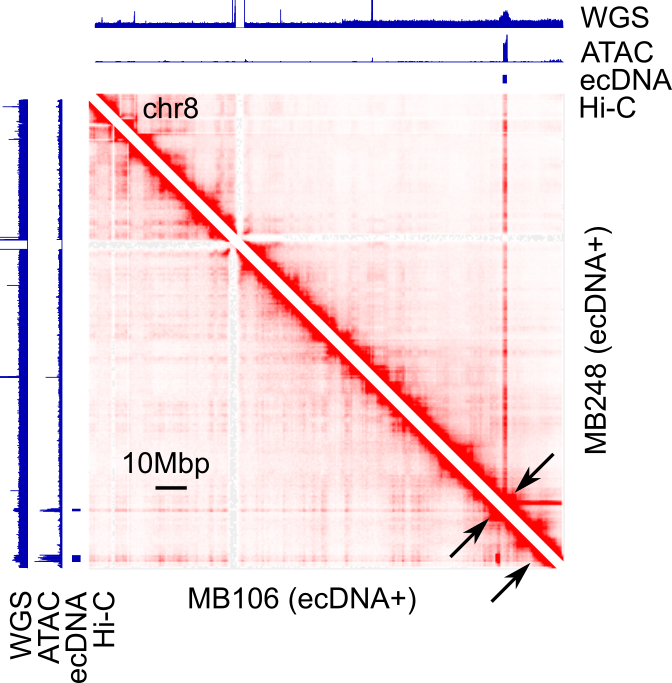
\includegraphics{MB106-MB248-chr8}
    \label{fig:MB106-MB248-hic}
    \caption[Chromatin interaction maps of chr8 in patient tumors with \textit{MYC} ecDNA.]{\textbf{Chromatin interaction maps of chr8 in patient tumors with \textit{MYC} ecDNA.} Chromosome-wide view of intrachromosomal interactions mapping to chr8 of the reference human genome. \Gls{wgs}, ATAC-seq and Hi-C sequencing depth are shown for two Group 3 MB samples harboring circular amplification of \textit{MYC}. Extrachromosomally amplified loci are indicated by arrows. These tumors are described further in \cite{archer_2017}.
    }
    \label{fig:mb106-mb248-myc-hic}
\end{figure}

\par In half of the analyzed ecDNA+ tumors (D458, MB106, MB268, and RCMB56), we observed clear evidence of aberrant chromatin interactions on ecDNA which spanned DNA breakpoints to link accessible loci and co-amplified genes from distal genomic regions. In the \textit{MYC}-amplified Group 3 MB primary tumor MB106, DNA interactions occurred between the \textit{MYC} locus and two co-amplified accessible regions located 13Mbp away on the reference genome, but 75kbp and 800kbp away on the ecDNA (Fig. \ref{subfig:MB106-circos}). Comparing the MB106 Hi-C interactome to that of MB288, a Group 3 MB primary tumor without ecDNA, we found that these chromatin interactions were specific to the MB106 ecDNA (Fig. \ref{subfig:MB106-MB288-hic}). 

\begin{figure}[!h]
    \begin{subfigure}{.49\textwidth}
        \centering
        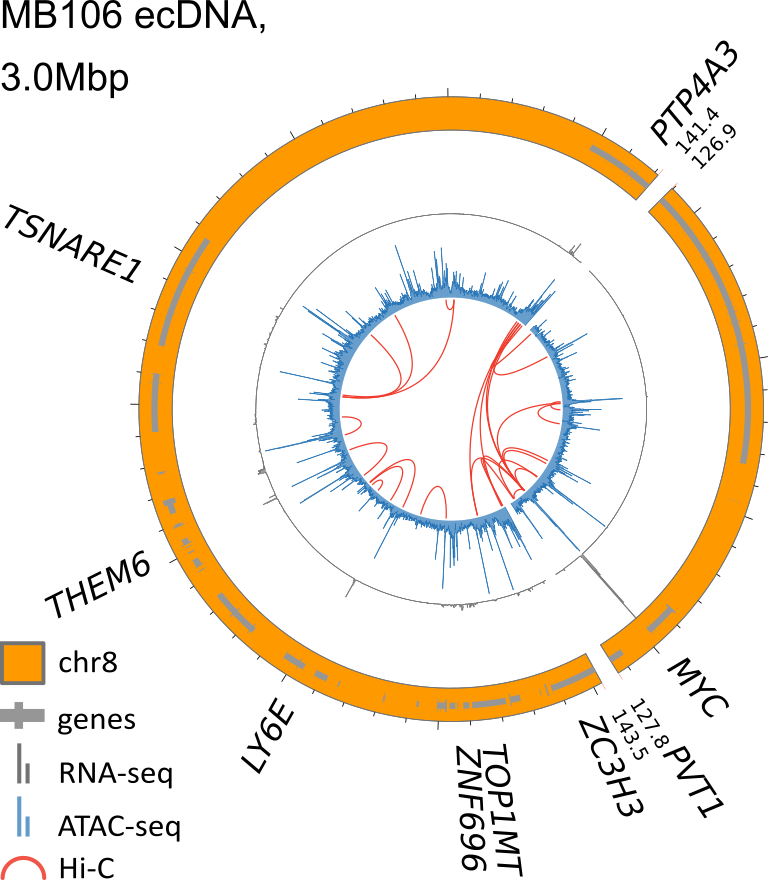
\includegraphics{MB106-circos}
        \caption{}
        \label{subfig:MB106-circos}
    \end{subfigure}
    \begin{subfigure}{.49\textwidth}
        \centering
        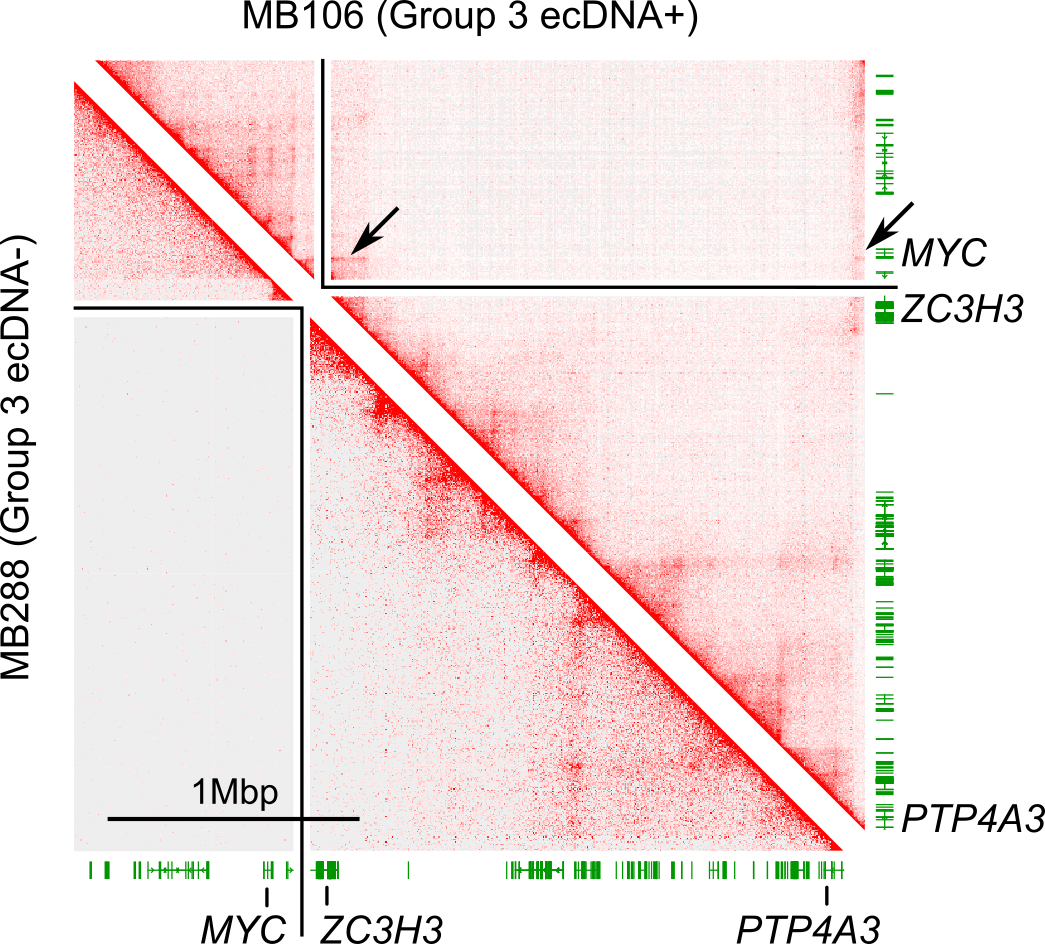
\includegraphics{MB106-MB288-ecDNA}
        \caption{}
        \label{subfig:MB106-MB288-hic}
    \end{subfigure}
    \caption[Transcriptional regulatory circuitry of ecDNA in \textit{MYC}-amplified Group 3 patient tumor MB106.]{\textbf{Transcriptional regulatory circuitry of ecDNA in \textit{MYC}-amplified Group 3 patient tumor MB106.} (\textbf{a}) Circular multi-omic map of the ecDNA sequence identified in Group 3 MB sample MB106. \textit{MYC} is highly expressed, and interacts with distal accessible loci located elsewhere on the ecDNA sequence. (\textbf{b}) Comparison of interaction densities at the MB106 ecDNA locus between MB106 (Group 3 ecDNA+) and MB288 (Group 3 ecDNA-). Ectopic interactions (arrows) between co-amplified segments of chr8 in MB106 are not present in the MB288 tumor with unrearranged \textit{MYC} locus.
    }
    \label{fig:MB106-MB288-myc-hic}
\end{figure}

In the SHH MB primary tumor MB268, we identified a 10.2Mbp ecDNA amplification which included the p53 regulator \textit{MDM4} \cite{toledo_2007} and is among the largest ecDNA amplifications identified in a patient tumor to date (Fig. \ref{fig:MB268}). \textit{MDM4} is recurrently amplified on glioblastoma ecDNA \cite{AA} and is a putative driver event in the MB268 tumor. On the same ecDNA, we also observed aberrant DNA interactions with the immune complement system regulator \textit{CFH} promoter. However, the functional significance of these co-amplified genes and DNA interactions remains unclear. 

\begin{figure}[!h]
    \centering
    \begin{subfigure}{.49\textwidth}
        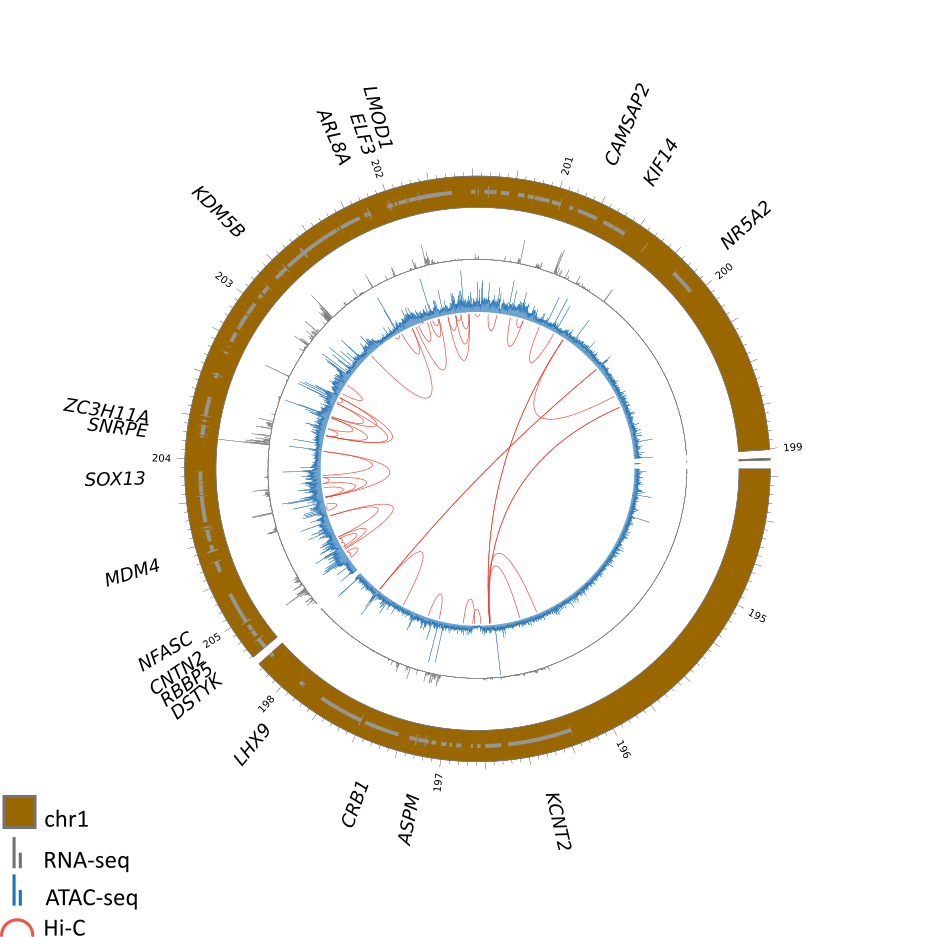
\includegraphics{MB268-circos}
    \end{subfigure}
    \begin{subfigure}{.49\textwidth}
        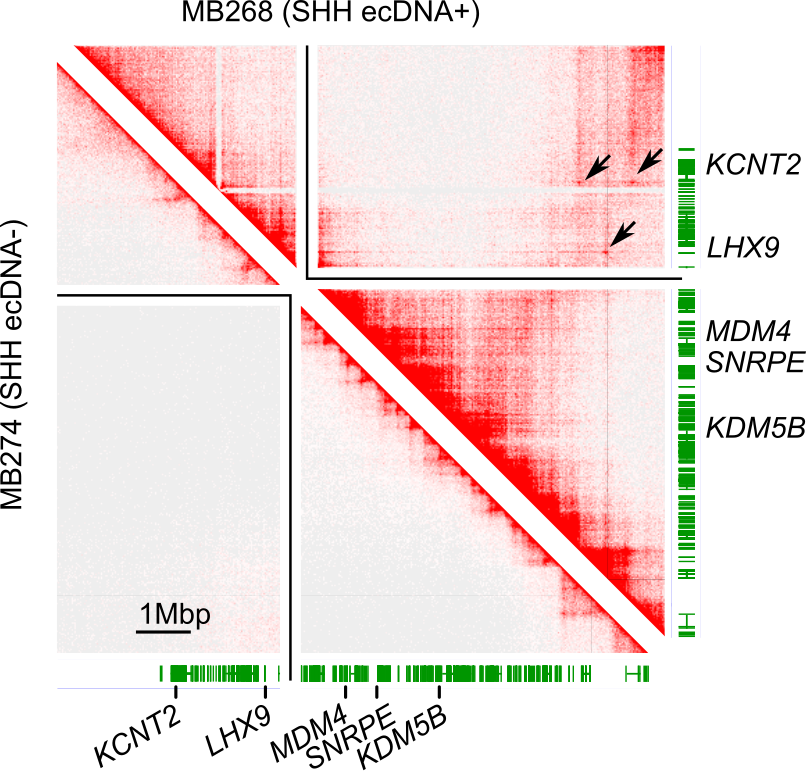
\includegraphics{MB268-hic}
    \end{subfigure}
    \caption[Transcriptional regulatory circuitry of ecDNA in SHH MB tumor MB268.]{\textbf{Transcriptional regulatory circuitry of ecDNA in SHH MB tumor MB268.} (\textbf{a}) Circular multi-omic map of the ecDNA present in the SHH MB patient tumor MB268. \textit{MDM4} is a negative p53 regulator recurrently amplified in glioblastoma \cite{AA}, and is a putative driver oncogene on this amplicon. (\textbf{b})Comparison of interaction densities at the MB268 ecDNA locus between MB268 (SHH ecDNA+) and MB274 (SHH ecDNA-). Ectopic interactions (arrows) between co-amplified segments of chr1 in MB268 are not present in unrearranged the MB274 tumor.
    }
    \label{fig:MB268}
\end{figure}

\par In two instances, the SHH MB tumor RCMB56-pdx and the Group 3 MB cell line D458, we identified rewired interactions between genomic loci originating from different chromosomes but co-amplified on the same ecDNA. As described above, RCMB56 harbored an ecDNA comprised of segments of chr1, and a complex extrachromosomal amplification comprised of segments of chr7 and chr17. Hi-C data indicated frequent chromatin interaction across breakpoints in each of the two amplicons present in this tumor (Fig. \ref{fig:RCMB56-circos}-\ref{fig:RCMB56-hic}). Aberrant chromatin interactions mapping to amp1 targeted accessible regions at the \textit{DNTTIP2}, \textit{SH3GLB1}, and \textit{SELENOF} gene loci (Fig. \ref{subfig:amp1-hic}). Aberrant interactions on amp2 included intrachromosomal interactions mapping to \textit{RPA3}, \textit{HERPUD2}, \textit{KLF14} and others; and trans-chromosomal interactions between the \textit{SP2} locus and the brain-specific long noncoding RNA \textit{LINC0301359}, and from the \textit{PRR15L} promoter to an intragenic region upstream of \textit{SRI} (Fig. \ref{subfig:amp2-hic}). 

\begin{figure}[!h]
    \centering
    \begin{subfigure}{.49\textwidth}
        \centering
        \includegraphics{RCMB56-amp1-circos}
        \caption{}
        \label{subfig:amp1-circos}
    \end{subfigure}
    \begin{subfigure}{.49\textwidth}
        \centering
        \includegraphics{RCMB56-amp2-circos}
        \caption{}
        \label{subfig:amp2-circos}
    \end{subfigure}
    \caption[Transcriptional regulatory circuitry of ecDNA sequences in RCMB56 p53-mutant SHH MB tumors.]{\textbf{Transcriptional regulatory circuitry of ecDNA sequences in RCMB56 p53-mutant SHH MB tumors.} (\textbf{a}) Transcription (RNA-seq, grey), accessible chromatin (blue), and chromatin interactions (Hi-C, red arcs) mapped onto the amp1 assembly (outer track, brown). Chromatin interactions occur across a structural breakpoint between accessible loci near highly-expressed genes such as \textit{DNTTIP2}. (\textbf{b}) Transcription, accessible chromatin, and chromatin interactions mapped onto the amp2 assembly. The gap in the assembly is adjacent to pericentromeric and peritelomeric loci. Ectopic interactions putatively target \textit{RPA3}, \textit{HERPUD2}, \textit{KLF14}, \textit{SP2}, and others.}
    \label{fig:RCMB56-circos}
\end{figure}
\begin{figure}
    \begin{subfigure}{\textwidth}
        \centering
        \includegraphics{RCMB56-amp1-hic}
        \caption{}
        \label{subfig:amp1-hic}
    \end{subfigure}
    \begin{subfigure}{\textwidth}
        \centering
        \includegraphics{RCMB56-amp2-hic}
        \caption{}
        \label{subfig:amp2-hic}
    \end{subfigure}
    \caption[Ectopic chromatin interactions on ecDNA in RCMB56.]{\textbf{Enhancer rewiring on ecDNA in RCMB56.} See also Fig. \ref{fig:RCMB56-circos}. (\textbf{a}) Chromatin interaction density map of the amp1 assembly. Arrows indicate putative enhancer rewiring events, or chromatin loops which span a breakpoint on the amp1 assembly. (\textbf{b}) Chromatin interaction density map of the amp2 assembly. Putative enhancer hijacking events are again indicated by arrows. The two ends of this assembly do not interact (top of the triangle), suggesting that they are spatially distant in the cell.}
    \label{fig:RCMB56-hic}
\end{figure}

\par D458 harbors an ecDNA amplification containing MB oncogenes \textit{MYC} and \textit{OTX2}, from chromosomes 8 and 14 respectively. Co-amplification of \textit{MYC} and \textit{OTX2} on the same ecDNA was validated by confocal FISH showing extrachromosomal co-localization of \textit{OTX2} and \textit{MYC} in D458 cells (Fig. \ref{D458-fish}), and by assembly of the D458 ecDNA from WGS and OGM data (Supplementary Fig. 11 of \cite{Chapman}). \textit{OTX2} is a known regulator of \textit{MYC} transcription and both genes are highly expressed in D458 (Fig. \ref{subfig:f4e}). The Hi-C data revealed several interactions of the \textit{MYC} promoter with co-amplified regulatory elements of chr8 and chr14 (Fig. \ref{fig:D458-ecDNA}). In summary, these results show that aberrant enhancer-promoter interactions resulting from structural rearrangements on ecDNA are common in MB tumors. 

\begin{figure}[!h]
    \centering
    \begin{subfigure}{\textwidth}
        \centering
        \includegraphics{D458-fish}
        \caption{}
        \label{D458-fish}
    \end{subfigure}
    \begin{subfigure}{.54\textwidth}
        \centering
        \includegraphics[right]{f4e}
        \caption{}
        \label{subfig:f4e}
    \end{subfigure}
    \begin{subfigure}{.44\textwidth}
        \centering
        \includegraphics[right=2cm]{D283-fish}
        \caption{}
        \label{subfig:D283-fish}
    \end{subfigure}
    \caption[Two Group 3 MB cell lines with intra- and extrachromosomal \textit{MYC} amplifications.]{\textbf{Two Group 3 MB cell lines with intra- and extrachromosomal \textit{MYC} amplifications.} (\textbf{a}) Confocal FISH of \textit{MYC} and \textit{OTX2} on a metaphase spread of a D458 cell. (\textbf{b}) Gene transcription of all protein-coding genes in D458 and D283 from publicly available data in DepMap \cite{depmap}.  MB Group 3 oncogenes \textit{MYC} and \textit{OTX2} are highlighted. (\textbf{c}) FISH in a metaphase spread of a D283 nucleus shows chromosomal \gls{HSR} \textit{MYC} amplification. \textit{OTX2} is not amplified in D283.}
    \label{fig:D458-fish}
\end{figure}

\begin{figure}[!h]
    \begin{subfigure}{\textwidth}
        \centering
        \includegraphics{D458-circos}
        \caption{}
        \label{subfig:D458-circos}
    \end{subfigure}
    \begin{subfigure}{\textwidth}
        \centering
        \includegraphics{D458-hic}
        \caption{}
        \label{subfig:D458-hic}
    \end{subfigure}
    \caption[Transcriptional regulatory map of the D458 ecDNA.]{\textbf{Transcriptional regulatory map of the D458 ecDNA.} (\textbf{a}) Circular map of accessible chromatin (blue) and chromatin interactions (red) mapping to the D458 ecDNA sequence assembly. 
    (\textbf{b}) Interchromosomal interactions between segments of the D458 ecDNA originating from chr8 and chr14. Arrows highlight putative chromatin loops included in (a). f: functional, as determined by a significant and D458-specific effect on cell proliferation upon CRISPRi inhibition (Fig. \ref{fig:crispri-pooled}); nf: not identified as functional in the same pooled CRISPRi screen.
    }
    \label{fig:D458-ecDNA}
\end{figure}

\subsection{Co-amplified enhancers shape the transcriptional regulatory circuitry of ecDNA.}
To test whether the observed enhancer rewiring events in ecDNA have functional roles in tumor cell proliferation, we performed a pooled CRISPRi proliferation screen in the Group 3 MB cell line D458, targeting all 645 accessible loci co-amplified on the ecDNA using 32,530 small guide RNA sequences (sgRNAs). These loci included 10 highly accessible regions from chr14, each overlapping ENCODE candidate cis-regulatory elements (cCREs) \cite{encode}. Because enhancer usage is highly conserved in Group 3 MB tumors \cite{lin_2017}, we performed the same screen in the Group 3 cell line D283, in which \textit{MYC} (but not \textit{OTX2}) is tandem amplified on a 55Mbp \gls{HSR} of chr8q (Fig. \ref{subfig:D283-fish}). While the \textit{MYC} promoter was essential in both cell lines, our screen identified 6 functional elements which, upon CRISPRi inhibition, specifically reduced D458 proliferation compared to D283 after 21 days (MAGeCK MLE, $q < 0.05$; Fig. \ref{fig:crispri-pooled}) \cite{mageck}. On chr8, these loci included two accessible regions of a known \textit{MYC} superenhancer \cite{lin_2017} and the \textit{PVT1} promoter. In D458, much of the superenhancer is duplicated internally on the ecDNA, and \textit{PVT1} is amplified in D458 but not in D283.  Conversely, we observed that other accessible regions of the same \textit{MYC} superenhancer were specifically essential for D283 but not for D458, indicating altered regulatory dependencies on the \textit{MYC}-ecDNA compared to the \textit{MYC}-HSR amplification. These results are consistent with a previous comparison of ecDNA+ and ecDNA- glioblastoma cell lines, where the impact of enhancer silencing on proliferation was associated with cell line-specific chromatin accessibility and interactions \cite{Morton_2019}.

The Hi-C data indicated interactions between \textit{MYC} on chr8 and regulatory elements of chr14 co-amplified on the same ecDNA, two of which are essential for D458 proliferation (Fig. \ref{subfig:D458-hic}): a cluster of elements at the \textit{OTX2} locus as well as a distal enhancer \cite{wortham_2014} located 80kbp downstream of \textit{OTX2} on the reference genome, but inverted on the ecDNA. D283-specific elements on chr14 included peaks at the N-terminal exon of \textit{OTX2} and another distal enhancer \cite{wortham_2014} 55kbp from \textit{OTX2} on the reference but also inverted on the ecDNA. To further test the influence on transcription of regulatory regions essential in D458 but not in D283, we performed additional CRISPRi inhibition experiments targeted against the \textit{PVT1} promoter and an accessible region within the internal duplication of the \textit{MYC} superenhancer. Consistent with the result of the CRIPSRi proliferation screen, silencing of the \textit{MYC} superenhancer reduced \textit{MYC} expression for 2 out of 3 tested sgRNAs in D458 but not in D283 (Fig. \ref{fig:crispri-myc-se}). No significant difference was observed in \textit{OTX2} transcription in either cell line. Silencing of the \textit{PVT1} promoter abrogated \textit{PVT1} transcription but not \textit{MYC} or \textit{OTX2}, in D458 but not in D283 (Fig. \ref{fig:crispri-pvt1-tss}). Thus, although proliferation in both Group 3 MB cell lines is driven by \textit{MYC} amplification, the relative importance of co-amplified genes and cis-regulatory elements is specific to the genomic architecture of the amplicon.

% Pooled CRISPRi screen
\begin{figure}[!h]
    \centering
    \centerline{%
    \includegraphics{pooled-screen}%
    }
    \caption[A large CRISPRi screen identifies differentially active enhancers in two \textit{MYC} amplicons.]{\textbf{A large CRISPRi screen identifies differentially active enhancers in two \textit{MYC} amplicons.} Pooled CRISPRi screen in the two G3 MB cell lines D458 (\textit{MYC} ecDNA) and D283 (\textit{MYC} HSR) targeted against all accessible loci on the D458 ecDNA as identified by ATAC-seq. Tracks from top to bottom: amplified regions of the D458 ecDNA; amplified regions of the D283 HSR; refSeq genes; D458 bulk ATAC-seq signal; CRISPRi essentiality score tracks for D458 and D283 generated by CRISPR-SURF \cite{crispr-surf}. Vertical highlighted bars indicate accessible loci which are significantly depleted at T21 relative to T0, and colored by cell line specificity. Grey: essential in D458 and D283 with no significant difference; green: significantly depleted in D458 relative to D283; yellow: significantly depleted in D283 relative to D458. All significance values determined by FDR-corrected MAGeCK-MLE permutation test \cite{mageck} ($q < 0.05$).}
    \label{fig:crispri-pooled}
\end{figure}

% Targeted CRISPRi of MYC SE
\begin{figure}[!h]
    \centering
    \begin{subfigure}{.49\textwidth}
        \centering
        \includegraphics{D458-MYC-SE-MYC}
        \caption{}
        \label{subfig:d458-myc-se-myc}
    \end{subfigure}
    \begin{subfigure}{.49\textwidth}
        \centering
        \includegraphics{D458-MYC-SE-OTX2}
        \caption{}
        \label{subfig:d458-myc-se-otx2}
    \end{subfigure}
    \begin{subfigure}{.49\textwidth}
        \centering
        \includegraphics{D283-MYC-SE-MYC}
        \caption{}
        \label{subfig:d283-myc-se-myc}
    \end{subfigure}
    \begin{subfigure}{.49\textwidth}
        \centering
        \includegraphics{D283-MYC-SE-OTX2}
        \caption{}
        \label{subfig:d283-myc-se-otx2}
    \end{subfigure}
    \caption[A co-amplified enhancer on the D458 ecDNA promotes \textit{MYC} expression.]{\textbf{A co-amplified enhancer on the D458 ecDNA promotes \textit{MYC} expression.} Relative expression of \textit{MYC} and \textit{OTX2} in D458 (\textbf{a}-\textbf{b}) and D283 (\textbf{c}-\textbf{d}), measured by qPCR ($2^{-\Delta\Delta Ct}$), in D458 and D283 cell lines upon CRISPRi targeting of an accessible locus within a known \textit{MYC} superenhancer which promotes D458 proliferation (see also Fig. \ref{fig:crispri-pooled}). sgNT: nontargeting control; sg\textit{MYC}-SE-A-C: sgRNAs targeting the \textit{MYC} enhancer at D458\_peak\_30782, positions chr8:127330655, chr8:127330840, and chr8:127330927 respectively. qPCR was performed on all guides in technical triplicate. All co-ordinates refer to the hg38 assembly. ** $p < 0.01$; *** $p < 0.001$; nested ANOVA with Dunnett’s correction.
    }
    \label{fig:crispri-myc-se}
\end{figure}

% Targeted CRISPRi of PVT1 TSS
\begin{figure}[!h]
    \centering
    \begin{subfigure}{.32\textwidth}
        \centering
        \includegraphics{D458-PVT1-TSS-PVT1}
        \caption{}
        \label{subfig:d458-pvt1-tss-pvt1}
    \end{subfigure}
    \begin{subfigure}{.32\textwidth}
        \centering
        \includegraphics{D458-PVT1-TSS-MYC}
        \caption{}
        \label{subfig:d458-pvt1-tss-myc}
    \end{subfigure}
    \begin{subfigure}{.32\textwidth}
        \centering
        \includegraphics{D458-PVT1-TSS-OTX2}
        \caption{}
        \label{subfig:d458-pvt1-tss-otx2}
    \end{subfigure}
    \begin{subfigure}{.32\textwidth}
        \centering
        \includegraphics{D283-PVT1-TSS-PVT1}
        \caption{}
        \label{subfig:d283-pvt1-tss-pvt1}
    \end{subfigure}
    \begin{subfigure}{.32\textwidth}
        \centering
        \includegraphics{D283-PVT1-TSS-MYC}
        \caption{}
        \label{subfig:d283-pvt1-tss-myc}
    \end{subfigure}
    \begin{subfigure}{.32\textwidth}
        \centering
        \includegraphics{D283-PVT1-TSS-OTX2}
        \caption{}
        \label{subfig:d283-pvt1-tss-otx2}
    \end{subfigure}
    \caption[\textit{PVT1} promotes D458 cell proliferation.]{\textbf{\textit{PVT1} promotes D458 cell proliferation.} 
     Relative expression of \textit{PVT1}, \textit{MYC}, and \textit{OTX2}, measured by qPCR ($2^{-\Delta\Delta Ct}$), in D458 (\textbf{a}-\textbf{c}) and D283 (\textbf{d}-\textbf{f}) cell lines upon CRISPRi targeting of the \textit{PVT1} promoter which promotes D458 proliferation (see also Fig. \ref{fig:crispri-pooled}). sgNT: nontargeting control; sg\textit{PVT1}-D-F: sgRNAs targeting the \textit{PVT1} promoter at D458\_peak\_30920, positions chr8:127794266, chr8:127794773, and chr8:127794945 respectively. qPCR was performed on all guides in triplicate. All co-ordinates refer to the hg38 assembly. *** $p < 0.001$; **** $p < 0.0001$; nested ANOVA with Dunnett’s correction.
    }
    \label{fig:crispri-pvt1-tss}
\end{figure}

\subsection{ecDNA interacts with chromosomal oncogene loci.}
Recent studies have revealed intermolecular enhancer-promoter interactions between ecDNA molecules (`ecDNA hubs') \cite{hung_2021} or between the chromosomes and ecDNA (`mobile enhancers') \cite{Zhu_2021}. To test for such intermolecular chromatin interactions in medulloblastoma, we computationally identified interchromosomal loops from Hi-C of the SHH MB tumor RCMB56-pdx, where one loop anchor mapped to the circular ecDNA amp1. This analysis revealed a nexus of interactions mapping from the \textit{ARHGAP29} locus on amp1 to loci elsewhere in the genome with plausible tumorigenic roles, including \textit{MECOM}, \textit{RAD51AP2}, \textit{POU4F1}, and \textit{IGF1R} (Fig. \ref{fig:mobile-enhancers}). However, the functional significance of these intermolecular chromatin interactions in MB remains untested.

% mobile enhancers
\begin{figure}[!h]
    \begin{subfigure}{.49\textwidth}
        \centering
        \includegraphics{RCMB56-amp1-trans-circos}
        \caption{}
        \label{subfig:RCMB56-amp1-trans}
    \end{subfigure}
    \begin{subfigure}{.49\textwidth}
        \centering
        \includegraphics{RCMB56-amp1-trans-hic}
        \caption{}
        \label{subfig:rcmb56-mecom}
    \end{subfigure}
    \caption[The RCMB56 amp1 ecDNA interacts with chromosomal gene loci.]{\textbf{The RCMB56 amp1 ecDNA interacts with chromosomal gene loci.} (\textbf{a}) Interchromosomal chromatin interactions detected by FitHiC2 \cite{fithic2} between amp1 and other chromosomes. Interactions mapping to a gene locus are labelled. (\textbf{b})  Interaction density map between segments of chr1 and chr3, rendered in Juicebox \cite{juicebox}. Vertical stripes indicate increased contact density between the ecDNA and chr3 over background interactions between chr1 and chr3. Arrow indicates the chromatin loop detected between \textit{ARHGAP29} on amp1 and \textit{MECOM} on chr3. 
    }
    \label{fig:mobile-enhancers}
\end{figure}

\section{Discussion}
    
By mapping chromatin interactions occurring on ecDNA in patient and model tumors, we observe ectopic chromatin interactions occurring between genomic loci which are distal on the reference genome but proximal on the ecDNA. In representative tumors of the SHH and Group 3 \gls{MB} subgroups, these interactions targeted known or putative oncogene loci, and coincided with high gene expression. To determine the extent to which the enhancer landscape of an ecDNA may affect cell proliferation, we performed pooled and targeted CRISPR inhibition experiments in the Group 3 MB cell line D458, which amplifies oncogenes \textit{MYC}, \textit{OTX2}, and \textit{PVT1} on ecDNA. These experiments reveal that a distal \textit{MYC} superenhancer is essential to cell proliferation, and that the relative importance of specific enhancer sub-elements is specific to the sequence of the structural rearrangement. In this illustrative model, the rearranged enhancer landscape of the ecDNA sequence contributes to the cell's proliferative capacity.

Therapeutic targeting of rewired enhancers in patient tumors remains a major unresolved challenge. In our example Group 3 \textit{MYC}-amplified cell lines D283 and D458, the bromodomain inhibitor JQ1 attenuates cell growth by downregulating \textit{MYC} transcription \cite{bandopadhayay_2014}. The mechanism of action is believed to be disruption of BRD4-mediated binding of transcriptional machinery to \textit{MYC} enhancers, downregulating \textit{MYC} expression. However, clinical trials of BRD inhibitors have so far shown high rates of adverse events and limited efficacy \cite{sun_2020}. In addition, further research will be required to resolve and target the exact oncogenic seuqences driving patient tumors such as RCMB56, which does not amplify a known MB oncogene on either ecDNA amplification.

\section{Methods}
\subsection{ATAC-seq}
Archer \textit{et al.} samples. At least 25mg of pulverized frozen tissue from samples previously included in proteomics analysis5 were sequenced by ATAC-seq according to an established protocol for bulk ATAC-seq of frozen neuronal cells\cite{milani_2016}. Reads were aligned, deduplicated and preprocessed according to ENCODE best practices. Samples included in subsequent analyses passed the following quality control thresholds: PCR bottleneck coefficient 1 (PBC1) $> 0.7$, PCR bottleneck coefficient 2 (PBC2) $> 3$, non-redundant read fraction (NRF) $> 0.8$ and TSS enrichment $> 2.6$. These samples had at least 13 million uniquely mapped single-end reads (GRCh37). Accessible chromatin regions were identified using MACS2 v2.1.2 \cite{macs} using Benjamini-Hochberg corrected p-value threshold $q< 0.05$.

\textit{RCMB56 and D458}. Frozen dissociated cells were ATAC-sequenced at ActiveMotif, Inc. (San Diego, CA). Briefly, ~100K cells were permeabilized and transposase loaded with sequencing adapters was added. Sequencing was performed on Illumina NextSeq 500. Reads were aligned, deduplicated and preprocessed according to ENCODE best practices. Samples had PBC1 $> 0.9$, PBC2 $> 20$, NRF $> 0.5$ and at least 30 million uniquely mapped paired-end reads (hg38). Accessible chromatin regions were identified using MACS2 v2.1.2 \cite{macs} using Benjamini-Hochberg corrected p-value threshold $q < 0.05$.
\subsubsection{Chromosome conformation capture}
\textit{Archer et al. samples (except MB248)}. Hi-C on frozen tumor tissue sample was carried out using protocols previously described for tissue Hi-C experiments88. In brief, frozen tissues are pulverized using a mortar and pestle kept cold on a bed of dry ice into a fine powder. The tissue powder was then transferred to a 15mL conical tube containing 5mLs of DPBS and fixed with 2\% formaldehyde for 10 minutes. The fixation was quenched by addition of 0.2M Glycine. The fixed tissue was pelleted by centrifugation, washed 1x with DPBS, and then flash frozen until ready for further processing. For Hi-C experiments, the fixed frozen tissue pellets were first resuspended in 3mLs of lysis buffer (10mM Tris-HCl pH 8.0, 5mM CaCl\textsubscript{2}, 3mM MgAc, 2mM EDTA, 0.2mM EGTA, 1mM DTT, 0.1mM PMSF, 1X Complete Protease Inhibitors). The sample was transferred to an M-tube and dissociated using a GentleMACS Tissue dissociator (Miltenyi) using the ``Protein M-tube'' setting. The sample was removed from the M-tube into a 50mL conical. The M-tube was washed with 3mLs of lysis buffer with 0.4\% Triton X-100 added, and this wash was combined with the original 3mLs of sample for a total volume of 6mLs with final concentration of 0.2\% Triton X-100. The sample was then passed through a 40µM cell strainer. The strainer was washed with an additional 2mLs of lysis buffer with 0.2\% Triton X-100. The sample was then centrifuged and washed with 1mL of lysis buffer with 0.2\% Triton X-100. After centrifugation, the sample was resuspended in 0.5\% SDS and processed with previously described in situ Hi-C method \cite{rao_2014} using the MboI enzyme. Libraries were prepared using the Illumina TruSeq LT sequencing adaptors. Initial QC sequencing was first performed on a MiSeq to assess library quality, and if sufficient, was subject to production scale sequencing on the HiSeq X or NovaSeq platform, respectively.

\textit{D458, RCMB56, and MB248}. Hi-C experiments were carried out by Arima Genomics, Inc (San Diego, CA) using the Arima-HiC Kit protocol with MboI restriction enzyme. Subsequently, Illumina-compatible sequencing libraries were prepared by shearing the proximally ligated DNA and then size-selecting DNA fragments using SPRI beads. The size-selected fragments containing ligation junctions were enriched using Enrichment Beads (provided in the Arima-HiC Kit), and converted into Illumina-compatible sequencing libraries using the Swift Accel-NGS 2S Plus kit (P/N: 21024) reagents. After adapter ligation, DNA was PCR amplified and purified using SPRI beads. The purified DNA underwent standard QC (qPCR and Bioanalyzer) and sequenced on the NovaSeq following manufacturer's protocols.

\subsection{Hi-C data processing}
Hi-C reads were trimmed using Trimmomatic 0.39 \cite{trimmomatic} and aligned to the hg38 human genome reference using the HiC-Pro toolkit v2.11.3-beta using default parameters\cite{hic-pro}. Visualization and contact normalization was performed with JuiceBox v1.11.08 \cite{juicebox} and the Knight-Ruiz algorithm \cite{kr}. Chromatin interactions were called using Juicer Tools GPU HiCCUPS v1.22.01 \cite{juicer} using fdr threshold 0.2 and default recommended parameters for Hi-C \cite{rao_2014}. From visual inspection, we found that HiCCUPS correctly annotated interactions mapping to ecDNA, except for locus pairs mapping within ~50kb of a structural rearrangement. Due to these technical challenges, chromatin interactions described herein were manually curated based on HiCCUPS interaction calls. 

\subsection{Identification of intermolecular chromatin interactions} 
See also \ref{fig:mobile-enhancers}. To screen for putative intermolecular chromatin interactions originating from possible mobile enhancers on ecDNA \cite{Zhu_2021}, we performed loop detection on Hi-C data of RCMB56-pdx using FitHiC v2.0.8 \cite{fithic2} inter-chromosomal mode, at resolution 50kbp and setting no bias upper bound, as recommended by the tool's authors for this task. Interactions with corrected q-values less than 0.05 were selected, then further filtered for loops with one anchor mapping to RCMB56 amp1. To reduce false positive loop calls originating from changes in copy number variation, loops were further filtered to remove those mapping to amp2 or to within 100kbp of a breakpoint on amp1. After filtering, 46 high-confidence loops remained which mapped from amp1 to elsewhere in the reference genome. Genes were associated with a loop if the gene locus overlapped the 50kbp loop anchor. Panel \ref{subfig:RCMB56-amp1-trans} was generated using circos v0.69-8 \cite{circos}.

\subsection{Pooled CRISPRi proliferation screen}
The pooled CRISPRi proliferation screen was designed according to methods described previously \cite{Morton_2019}. Briefly, sgRNAs targeting the D458 ecDNA regulome were designed using CHOPCHOP \cite{chopchop}. All sgRNAs with no exact homology elsewhere in the genome (ie, mm0 = 0) were included, totaling 32,530 sgRNAs. Targeted regions included 645 accessible regions on the D458 ecDNA, and putative enhancers of \textit{MYC} in medulloblastoma61. As positive controls, sgRNAs targeting the promoter regions of \textit{POLR2A}, \textit{MYC} and \textit{OTX2} were also included. No non-targeting sgRNAs were included; however 4 1kbp loci from chr8 with no evidence of regulatory activity in D458 were also included. Pooled oligonucleotides were generated at Genewiz, Inc. The library was amplified and packaged into lentivirus in 293FT cell line (Invitrogen) by SBP Functional Genomics Core Facility.

D283 Med and D458 Med cells were infected by the lentivirally-packaged sgRNA library at a MOI of 0.3 at a multiplicity of 1000 cells/sgRNAs. Two independent infections were performed for each cell line as biological replicates (A and B). Forty-eight hours post-infection, infected cells were selected using puromycin (1\textmugreek g/ml). After 2 days selection, the MOI was measured and 30 million of cells were collected for NGS sequencing (timepoint 0 ``T0'') as a reference baseline for sgRNA distribution. Another 30 million of cells were re-plated into the culture flasks and maintained for 21 days (timepoint 21 ``T21''). 

To ensure sgRNA representation in each replicate, 30 million cells were maintained throughout the screen during cell passage every 3-4 days. Cells were harvested at T21, and genomic DNA extraction was performed using the NucleoSpin Blood XL kit. The NGS samples were prepared by the SBP Functional Genomics Core Facility using two-step PCR amplification of the integrated sgRNA using the genomic DNA as a template. For the first PCR, ``PCR1'' sgRNAs were amplified using Herculase II Fusion DNA Polymerases (Agilent 600675) from total genomic DNA isolated from each replicate at T0 and T21. 4\textmugreek g of genomic DNA was used for each 50ul reaction. PCR1 products were cleaned up using QIAquick PCR Purification Kit (Qiagen). For the second PCR ``PCR2'', 5 \textmugreek l of each cleaned PCR1 product was used for each 50\textmugreek l reaction with primers designed to include Illumina Adaptors and unique barcodes to allow for multiplexed NGS. PCR2 products were bead-purified (AMPure XP, Beckman), and eluted in 30 \textmugreek l of low-EDTA TE buffer. Final concentrations of the desired products were determined by TapeStation (Agilent) and equimolar amounts from each sample were pooled for Next Generation Sequencing.
Following selection, libraries were sequenced on an Illumina NovaSeq 6000 to a minimum depth of 60M reads per sample. Sequencing data QC, alignment and preprocessing was performed using MAGeCK-VISPR v0.4.165 \cite{mageck} At least 85\% of reads per sample were uniquely mappable to a sgRNA sequence, and fewer than 100 sgRNAs (0.3\%) were absent from any library. CRISPRi score tracks were generated using CRISPR-SURF v1.06 \cite{crispr-surf}. To identify D458-specific functional loci, T21 and T0 for both cell lines were compared using the Robust Rank Aggregation (RRA) algorithm of MAGeCK. Essential loci were identified for each cell line where guides mapping to that locus were depleted at T21 (corrected p-value $< 0.05$). Independently, D458-specific loci were identified by a linear model parameterized on cell line and timepoint (MAGeCK MLE, corrected p-value $< 0.05$). The final set of D458-specific functional loci was the intersection of the loci identified by these two analyses. Genomic tracks were plotted in IGV desktop v2.9.2 \cite{igv}.

\subsection{Targeted CRISPRi experiments}
For CRISPRi experiments, D283 and D458 medulloblastoma cells were lentivirally transduced with dCas9-KRAB-mCherry plasmid \cite{crispri} (Addgene \#60954) to express dCas9 in these cells. Cells stably expressing dCas9 were FACS sorted based on mCherry expression and were transduced with sgRNA vectors. sgRNAs were cloned into the lentiGuide-puro plasmid (Addgene \#52963) as described previously \cite{dixit_2021}. All plasmids were verified by Sanger sequencing. 293T cells (ATCC Cat\# CRL-3216) were used to generate lentiviral particles by cotransfecting the packaging vectors psPAX2 and pMD2.G using LipoD293 transfection reagent (SignaGen, SL100668) following the manufacturer's instructions.

\subsection{Quantitative RT-PCR}
Five days after sgRNA transduction, cells from different conditions were collected and Qiagen RNeasy Kit was used to isolate total cellular RNA from cell pellets according to the manufacturer's instructions. iScript cDNA Synthesis Kit (Bio-Rad, catalog 1708890) was used for reverse transcription into cDNA. Quantitative real-time PCR was performed in technical triplicate for 2 bioreplicates of each experimental condition on a Bio-Rad CFX384 Real-Time System using SYBR Green PCR Master Mix (Bio-Rad, catalog 1725270). 
Gene transcription was estimated from qPCR data using the delta delta Ct method ($Exp = 2^{-\Delta \Delta Ct}$). Testing for change in gene expression was performed using nested ANOVA with Dunnett's multiple comparisons test, implemented in GraphPad Prism 9.5.2.

\section{Acknowledgments}

\ackfunding

\par Chapter 3, in full, is adapted from the following manuscript currently being prepared for publication: "Circular extrachromosomal DNA promotes inter- and intratumoral heterogeneity in high-risk medulloblastoma." Chapman, Owen; Luebeck, Jens; Sridhar, Sunita; Wong, Ivy T.L.; Dixit, Deobrat; Wang, Shanqing; Prasad, Gino; Rajkumar, Utkrisht; Pagadala, Meghana; Larson, Jon D.; He, Britney J.; Hung, King L.; Lange, Joshua T.; Dehkordi, Siavash R.; Chandran, Sahaana; Adam, Miriam; Morgan, Ling; Wani, Sameena; Tiwari, Ashutosh; Guccione, Caitlin; Lin, Yingxi; Dutta, Aditi; Lo, Yan Yuen; Juarez, Edwin; Robinson, James T.; Malicki, Denise M.; Coufal, Nicole G.; Levy, Michael; Hobbs, Charlotte; Scheuermann, Richard H.; Crawford, John R.; Pomeroy, Scott L.; Rich, Jeremy; Zhang, Xinlian; Chang, Howard Y.; Dixon, Jesse R.; Bagchi, Anindya; Deshpande, Aniruddha J.; Carter, Hannah; Fraenkel, Ernest; Mischel, Paul S.; Wechsler-Reya, Robert J.; Bafna, Vineet; Mesirov, Jill P.; Chavez, Lukas. The dissertation author was the primary investigator and author of the manuscript.
\chapter{\pedpancantitle}
\label{chap:pedpancan}

\section{Abstract}

Circular extrachromosomal DNA (ecDNA) is a driver of oncogene amplification in aggressive cancers. The frequency and diversity of ecDNA has been comprehensively described in many different types of adult cancers and in some selected childhood cancer types, such as neuroblastoma and medulloblastoma. However, the frequency of ecDNA and its association with survival has not been comprehensively analyzed in the spectrum of pediatric cancers. In this study, we used the Amplicon Architect (AA) bioinformatics tool via cloud computing to reconstruct ecDNA sequence structures from Whole Genome Sequencing (WGS) data available in two of the largest publicly accessible pediatric cancer data repositories, the Children's Brain Tumor Network (CBTN) and the St. Jude Cloud cancer genomics platform. In total, we analyzed a retrospective cohort of over 1,600 tumor biopsies from 1,400 different patients, spanning 47 different childhood tumor types. As a result, we identified ecDNA in 15 different pediatric tumor types, with an overall incidence of ecDNA of 10\% in the entire patient cohort. We estimate frequencies of ecDNA in pediatric osteosarcomas (47\%), rhabdomyosarcomas (40\%), retinoblastomas (19\%), ETMRs (all, $n=4$), high-grade gliomas (20\%), and others. Across this cohort, ecDNA was found to be significantly associated with poor survival. Our results show that ecDNA is widely prevalent in pediatric cancers, amplifies known and potentially novel oncogenes, frequently evolves during disease progression, and significantly associates with worse clinical outcomes.

\section{Introduction}

Circular extrachromosomal DNA (ecDNA) has recently emerged as a mechanism for rapid oncogene amplification. Also known as double minutes, ecDNA sequences are typically greater than 1 Mb in size, contain one or more oncogenic sequences, and lack centromeres. ecDNA is subject to non-Mendelian inheritance, leading to unequal segregation of ecDNA during cytokinsesis and consequently intratumoral heterogeneity with every cell division \cite{bafna_2022}. The mechanisms which promote and maintain ecDNA or which suppress or inhibit ecDNA have yet to be fully elucidated. Several methods have emerged for identification of ecDNA, including microscopic examination with FISH and sequencing-based approaches. Algorithmic assembly from short-read whole genome sequencing has arisen as a cost-effective method to identify ecDNA, and has been applied to estimate the prevalence of ecDNA in adult \cite{Kim_2020,pongor_2023,luebeck_2022} and some pediatric cancer types \cite{Koche_2020,Chapman}. However, we are aware of only isolated meta-analyses \cite{gebhart_2005} and case reports describing ecDNA in other pediatric solid tumors including rhabdomyosarcoma, osteosarcoma, retinoblastoma, and others. 

We and others have recently shown that many pediatric cancers harbor unique mutations and driver oncogenes that differ from their adult counterparts \cite{grobner_2018,ma_2018}. However, ecDNA analysis was not included in these pan-cancer studies, in part because computational methods for reconstructing ecDNA from whole-genome sequencing data were not available at the time.  To address this gap, we have now analyzed the frequency of ecDNA in two of the largest publicly available childhood cancer data repositories. The pediatric pan-cancer study presented here identifies childhood cancer types commonly affected by ecDNA, catalogues ecDNA-amplified genes in primary and recurrent tumors, and examines the association between ecDNA and patient survival. In addition to being an indicator of prognosis, ecDNA provides an opportunity for therapies targeting ecDNA-specific properties, but its real-time clinical applicability has yet to be explored. This study seeks to take the first step in this process by highlighting the spectrum of childhood patients who may benefit from future therapies targeting ecDNA. 

\section{Results}

\subsection{ecDNA occurs in at least 15 distinct pediatric tumor types.}

To investigate the prevalence of ecDNA in pediatric tumors, we accessed whole genome sequencing data from two large cloud genomic platforms: St Jude Cloud and Children’s Brain Tumor Network (CBTN). In total, we analyzed a retrospective cohort of \gls{wgs} data of 1670 tumor biopsies from 1481 different patients. Clinical data was available for some patients and included age at diagnosis, sex, survival, tumor tissue site, race/ethnicity, and molecular subgroup for some tumor types. To detect ecDNA, we applied AmpliconArchitect (AA), a tool that detects and reconstructs focal genomic amplifications from whole genome sequencing data \cite{AA}. We then applied AmpliconClassifier, which classifies the reconstructed sequence as ecDNA or a separate noncircular amplification. Amplicons were classified as circular, breakage-fusion-bridge, complex noncyclic, or linear (Fig. \ref{subfig:cloud-workflow-diagram}). 174 ecDNA sequences were detected in tumor tissue of 157 out of 1486 patients (10\%). This cohort spans 47 different tumor types, 15 of which were found to have ecDNA in at least one sample. The frequencies of ecDNA in these 15 cancer types were as follows: \acrfull{ETMR} 4/4 (100\%), \acrfull{PB} 2/4 (50\%), \acrfull{OS} 27/57 (47\%), \acrfull{RMS} 14/35 (40\%), \acrfull{CPC} 1/3 (33\%), \acrfull{NB} 32/106 (30\%), \acrfull{MPNST} 1/4 (25\%), \acrfull{HGG} 32/157 (20\%), \acrfull{RB} 6/32 (19\%), \acrfull{MB} 25/177 (14\%), \acrfull{ACC} 2/21 (10\%), \acrfull{EPN} 2/73 (3\%), \acrfull{CPG} 1/39 (3\%), \acrfull{GG} 1/44 (2\%), and \acrfull{LGG} 1/290 (0.3\%) (Fig. \ref{subfig:pedpancan-piecharts}). ecDNA was significantly associated with tumor type ($\chi^2 = 299.96$, p value $2.2\times10^{-16}$).  ecDNA was not identified in the 32 other tumor types in our cohort.

\begin{figure}[!h]
    \centering
    \begin{subfigure}{\textwidth}
        \centering
        \includegraphics{cloud-workflow-diagram}
        \caption{}
        \label{subfig:cloud-workflow-diagram}
    \end{subfigure}
    \begin{subfigure}{\textwidth}
        \centering
        \includegraphics{pedpancan-piecharts}
        \caption{}
        \label{subfig:pedpancan-piecharts}
    \end{subfigure}
    \caption[Frequency of ecDNA sequences across a large restrospective cohort of pediatric tumors.]{\textbf{Frequency of ecDNA sequences across a large restrospective cohort of pediatric tumors.} (\textbf{a}) Analysis workflow diagram of cloud cancer genomics databases of whole genome sequencing data. (\textbf{b}) ecDNA frequencies for select tumor types in this cohort.}
    \label{fig:frequency-pedpancan}
\end{figure}

\subsection{ecDNA status is predictive of 5-year survival across pediatric cancer types.}
To evaluate the relationship between ecDNA and survival across pediatric cancer types, we performed Kaplan-Meier regression analyses across 345 patients for whom clinical metadata were available. Patients with \gls{ecDNA+} tumors had significantly worse five-year overall and progression free survival compared to patients with ecDNA negative tumors (log-rank-test, $p_{OS} < 0.001$, $p_{PFS} < 0.001$) (Fig. \ref{fig:survival-pedpancan}). Individual survival analyses for each tumor type were not significant, attributable to low statistical power. To further substantiate the association between survival and ecDNA status, we performed a Cox regression analysis with ecDNA as the predictor and age and sex as covariates. ecDNA was significantly associated with poor survival ($HR=3.17$, $p = 1.24 \times 10^{-9}$). To determine whether \gls{ecDNA+} tumors had worse outcomes than those with other forms of focal amplification, we compared survival across different classes of amplification: no amplicon, ecDNA, linear, and highly rearranged amplicons). Patients with cyclic amplification had significantly worse overall survival compared to patients with no amplification and linear amplification (\comment{TODO}log-rank test, $p_{OS} < 0.001$). 

\begin{figure}[!h]
    \centering
    \begin{subfigure}{\textwidth}
        \centering
        \includegraphics{km-pedpancan}
        \caption{}
        \label{subfig:km-pedpancan}
    \end{subfigure}
    \begin{subfigure}{\textwidth}
        \centering
        \includegraphics{cph-pedpancan}
        \caption{}
        \label{subfig:cph-pedpancan}
    \end{subfigure}
    \caption[Survival analysis of a retrospective cohort of 345 patients across \textit{n} pediatric tumor types.]{\textbf{Survival analysis of a retrospective cohort of 345 patients across \textit{n} tumor types.} (\textbf{a}) Kaplan-Meier curves indicating 5-year overall survival for ecDNA+ and ecDNA- patients. (\textbf{b}) Cox Proportional Hazards regression coefficients indicating log relative hazards for age, sex, ecDNA status and tumor type.}
    \label{fig:survival-pedpancan}
    % TODO Update n of patients and tumor types in this analysis
\end{figure}

Molecular subgroup annotations were available for 108 for \gls{HGG} tumors, facilitating comparison of the effect size of ecDNA on survival relative to other molecular determinants of risk. The most current subgrouping of \gls{HGG} includes classification into \gls{H3K27mut}, \gls{H3G34mut}, \gls{IDHmut} and \gls{H3/IDHwt} tumors \cite{mackay_2017}. ecDNA was distributed across these subgroups as follows: \gls{H3K27mut} (14/56, 25\%), \gls{H3G34mut} (0/4, 0\%), \gls{IDHmut} (2/6, 33\%), and \gls{H3/IDHwt} (11/42, 26\%). Cox regression indicates that molecular subgroup, especially H3K27 mutation status, is a major determinant of patient outcome ($HR = 4.39$, $p < 0.001$), consistent with previous results \cite{mackay_2017}. This model estimates a modest but insignificant effect of ecDNA on patient survival ($HR = 1.13$, $p = 0.6$, Fig. \ref{fig:survival-hgg}).

\begin{figure}[!h]
    \centering
    \begin{subfigure}{\textwidth}
        \centering
        \includegraphics{km-hgg}
        \caption{}
        \label{subfig:km-hgg}
    \end{subfigure}
    \begin{subfigure}{\textwidth}
        \centering
        \includegraphics{cph-hgg}
        \caption{}
        \label{subfig:cph-hgg}
    \end{subfigure}
    \caption[Survival analysis of a retrospective cohort of 108 pediatric \gls{HGG} patients.]{\textbf{Survival analysis of a retrospective cohort of 108 pediatric \gls{HGG} patients.} (\textbf{a}) Kaplan-Meier curves indicating 5-year overall survival for ecDNA+ and ecDNA- patients. (\textbf{b}) Cox Proportional Hazards regression coefficients indicating log relative hazards for ecDNA status and tumor type.}
    \label{fig:survival-hgg}
\end{figure}

\subsection{ecDNA most commonly amplifies \textit{MYCN} in neuroblastoma.} 
\label{NB}
The genomic landscape of ecDNA in neuroblastoma has been thoroughly described \cite{Koche_2020, yi_2022}, and the distribution of ecDNA in this neuroblastoma patient cohort is largely consistent with previous observations. We identify circular ecDNA amplification in 32 out of 106 neuroblastomas (30\%). ecDNA amplification was almost exclusively detected at the \textit{MYCN} oncogene locus (30 out of 31, 97\%). 

\subsection{ecDNA amplifies C19MC-\textit{TTYH1} fusions in \acrlong{ETMR}.} Nine out of ten \gls{ETMR} tumors harbor oncogenic amplification and fusion of \textit{TTYH1} with the C19MC microRNA cluster \cite{li_2009, lambo_2019}. Our cohort includes 4 \gls{ETMR} tumors, all \textit{TTYH1}-C19MC amplified on ecDNA. One of these also had noncircular \textit{MYCN} amplification, suggesting a secondary driver.

\subsection{\textit{MYC} amplification occurs on ecDNA in \acrlong{PB}} \Glspl{PB} comprise five molecular subgroups, including a subgroup harboring recurrent amplification of \textit{MYC} \cite{li_2020}. We identify 2 ecDNA sequences in 4 \gls{PB} patient tumors, one amplifying \textit{MYC} and the other the C19MC cluster canonically amplified in \gls{ETMR}. It remains unknown whether the C19MC-amplified \gls{PB} shares other molecular or clinical features with \gls{ETMR} tumors.

\subsection{ecDNA amplifies diverse \acrlong{RMS} oncogenes including \textit{FOXO1}-\textit{PAX7} fusions.}
ecDNA has been described in \gls{RMS} case reports since 1971 \cite{granberg_1971, steilen-gimbel_1996, meddeb_1996, gil-benso_2003, mysorekar_2008}. A review of case literature  \cite{gebhart_2005} identifies ecDNA in 15\% of human rhabdomyosarcomas ($n=84$). We identify ecDNA in \gls{wgs} of 14 out of 35 \gls{RMS} tumors (40\%). Amplified oncogenes were \textit{SOX21} (putative, $n=3$), \textit{MYCN} ($n=2$), \textit{FGFR1} (2), \textit{MDM2} (2), \textit{NSD3} (2), and \textit{FOXO1}-\textit{PAX7} fusion (2). One ecDNA  sequence did not contain any known oncogenes. Both \textit{MYCN} amplification  \cite{williamson_2005} and \textit{FOXO1} fusion \cite{missiaglia_2012} are prognostic indicators of poor \gls{RMS} patient outcomes; however it remains unknown whether properties of ecDNA contribute to these outcomes.

\subsection{Half of focal amplifications in \acrlong{OS} are circular.}
Osteosarcomas have among the highest rates of structural variation among pediatric cancer types \cite{pcgp}, and over 90\% carry inactivating mutations of the p53 pathway \cite{chen_2014}. A previous case literature review reported ecDNA in 21\% of OS tumors ($n=146$) \cite{gebhart_2005}. We detect ecDNA in \gls{wgs} of 27 out of 57 OS patient tumors (47\%). The genomic distribution of ecDNA amplifications largely reflected the known regions of recurrent focal amplification in OS, including \textit{MYC} ($n=4$ patients) \textit{RUNX2} ($n=3$), and chr17p11.2-p12 ($n=6$). chr17p11.2-p12 contains unstable low-copy repetitive sequences which are amplified in pediatric  \gls{OS} \cite{van_dartel_2002} and \gls{MB} \cite{Chapman}, and adult \gls{HGG} \cite{van_dartel_2003}, \gls{MM} \cite{fabris_2007}, \gls{LMS} and \gls{MFH} \cite{kaur_2007}. Genes with putative oncogenic roles within this region include \textit{PMP22}, \textit{COPS3}, \textit{TOP3A}, \textit{MAPK7}, and \textit{MAP2K4} \cite{van_dartel_2002}. 

\subsection{ecDNA amplifies the known landscape of focal amplifications in pediatric \acrfull{HGG}}
Among adult patient tumors, ecDNA occurs most frequently in glioblastomas \cite{Kim_2020}. Reconstruction of circular ecDNA from \gls{wgs} of a large cohort of adult glioblastomas previously identified recurrent ecDNA amplification of \textit{EGFR}, \textit{MDM2}, \textit{CDK4} and \textit{MYCN} in descending frequency \cite{sanborn_2013}. In a large cohort of pediatric \gls{HGG}, also included in our dataset, focal amplification was previously reported of oncogenes \textit{PDGFRA}, \textit{MET}, \textit{EGFR}, \textit{MYC}, \textit{MYCN}, Cyclin D family members \textit{CCND1/2/3}, and Cyclin D-dependent kinases \textit{CDK4/6}. The circular structure of one of these amplicons (\textit{EGFR}) was subsequently comprehensively described at diagnosis and relapse \cite{xu_2019}. We identify ecDNA in 32 of 157 \glspl{HGG} (20\%). Circular amplicons included all of the oncogenes previously described as amplified in this cohort, establishing  circular ecDNA as a frequent form of oncogenic amplification in \gls{HGG}.
% Fusion genes?

\subsection{\textit{MYCN} amplification occurs on ecDNA in a high-risk subset of ependymomas.}
Amplification of the \textit{MYCN} oncogene defines a subset of \gls{EPN} tumors with exceptionally poor prognoses \cite{ghasemi_2019}. Given that in neuroblastoma, \textit{MYCN} is almost exclusively amplified on ecDNA and confers poor prognosis, we investigated whether \textit{MYCN} amplification can occur on ecDNA in \gls{EPN}. We identify 2 ecDNA sequences across 73 \gls{EPN} tumors. This cohort included a single patient with \textit{MYCN}-amplified spinal \gls{EPN}, where \textit{MYCN} was amplified on circular ecDNA in both primary and progressive tumors. The other ecDNA comprised amplification of segments of chr13q33, which to our knowledge has not been described in \gls{EPN}, but is amplified in other cancers \cite{knuutila_1998}. Genes with putative oncogenic roles within this amplicon include \textit{ITGB1L1} \cite{wang_2022}, \textit{ZIC2} \cite{liu_2022} and \textit{ZIC5} \cite{tan_2022, song_2022}.

\subsection{ecDNA amplifies \textit{RB1} fusion genes in RB.}
\Gls{RB} is generally distinguished by early biallelic inactivation of the \textit{RB1} tumor suppressor gene followed by subsequent driver mutations, but 3\% of non-hereditary \glspl{RB} carry wild-type \textit{RB1} and high-copy amplification of \textit{MYCN} \cite{rushlow_2013}. Other high-copy focal amplifications previously reported in \gls{RB} include \textit{MDM4} and co-amplification of \textit{OTX2} and \textit{AKT1} \cite{sakai_1985}. Given that \textit{MYCN}-amplified \gls{RB} bears histological resemblence to \gls{NB} \cite{rushlow_2013}, and that \textit{MYCN} amplifications occur almost exclusively on ecDNA in \gls{NB} (see \ref{NB}), we hypothesized that \textit{MYCN} amplification in \gls{RB} also occurs on ecDNA. We identify circular ecDNA in 6 of 32 \gls{RB} patient tumors. Two of these harbored \textit{MYCN} amplification on ecDNA, out of 3 total \textit{MYCN}-amplified \gls{RB} tumors. Other notable oncogenes amplified on ecDNA included \textit{OTX2} ($n=1$), \textit{SMARCA5} ($n=1$), and putative \textit{RB1} fusion genes ($n=2$): \textit{RB1-THSD1} and \textit{RB1-LHFPL6}. Both amplicons fused the 5' end of \textit{RB1} to the 3' end of the partner gene. No RNA-seq data were available to confirm expression of the putative fusion gene product. However, the recurrent high-copy amplification of truncated \textit{RB1}, and the absence of a high-confidence oncogene on either amplicon, make it tempting to speculate that the \textit{RB1} fusion products provide some other selective advantage beyond \textit{RB1} inactivation.

% \subsection{ecDNA was not detected in low-risk pediatric solid tumor types.}
% ecDNA was not detected in WT, PCP, etc. 
% ecDNA was detected in less than 5% of ...
% any observations about trends (could also be discussion).

\section{Discussion}

Our survey of circular ecDNA across a large cohort of many different pediatric tumor types reveals that ecDNA is most frequent in high-risk malignant tumors, and largely absent from low-risk or benign tumors. For example, ecDNA was detected in one in five high-grade gliomas, but only one in 290 low-grade gliomas. The landscape of ecDNA-amplified genes largely reflects previously-known landscapes of gene amplification, indicating that the oncogenic sequence is not only amplified, but circular and acentric as well. Similarly to a recent result in adult cancers, patients with tumors harboring circular acentric amplifications had worse five-year survival than patients with other forms of amplification.

\par Recurrently ecDNA-amplified genomic loci in other pediatric tumor types span the spectrum of known oncogenes in pediatric cancer: \textit{MYC} family proto-oncogenes, cyclin-dependent kinases, C19MC, growth factor receptors, and others. We highlight unanswered questions around a few recurrent ecDNA loci as promising areas of future study.

\par The chromosomal band chr17p11.2-p12 is ecDNA-amplified in 6 \gls{OS} and 1 \gls{MB} tumors in our cohort, and its amplification has been described in various adult cancers. Copy number variation in this region has also been shown to cause the childhood developmental disorders \gls{SMS} (deletion) \cite{gropman_2006} and \gls{CMT1A} (tandem duplication) \cite{thomas_1997}. The mechanism underlying both syndromes is believed to be unequal crossing over due to homologous recombination between flanking repeat gene clusters \cite{potocki_2000}. It remains to be shown whether the ecDNA amplifications at that locus arise by a similar mechanism.

\section{Methods}

\subsection{Pediatric Tumor WGS}

\subsubsection{CBTN – Children’s Brain Tumor Network (992 biosamples from 831 patients)} WGS of a variety of pediatric tumor biopsies were identified using the Gabriella Miller Kids First Data Resource center portal (\url{https://portal.kidsfirstdrc.org/}). Patients were originally sequenced as part of the Pediatric Brain Tumor Atlas (PBTA) (\url{https://cbtn.org/pediatric-brain-tumor-atlas}). WGS data were preprocessed and aligned to human reference genome hg38 using the Kids First harmonized WGS pipeline (\url{https://github.com/kids-first/kf-somatic-workflow}) and subsequently analyzed using Cavatica (\url{https://cavatica.sbgenomics.com/}), on the cloud genomic analysis platform for Kids First genomic data. Docker containers containing fingerprint and AmpliconArchitect software were installed on the Cavatica cloud genomics platform (see section \ref{4-classification}).

\subsubsection{St. Jude – St Jude Cloud Repository (678 biosamples from 655 patients)} WGS of pediatric tumor biopsies were identified using the St Jude Cloud data portal. Patients were sequenced as part of the \gls{pcgp} and \gls{rtcg}. AmpliconArchitect software was installed on the SJ Cloud platform (see section \ref{4-classification}). 

\subsection{ecDNA detection and classification from bulk WGS}
\label{4-classification}
To detect ecDNA, all samples in the WGS cohort were analyzed using AmpliconArchitect v1.2 \cite{AA} and AmpliconClassifier v0.4.4 \cite{Kim_2020}. Briefly, the AmpliconArchitect algorithm was performed as follows. Copy number segmentation and estimation were performed using CNVkit v0.9.667 \cite{cnvkit}. Segments with copy number $ CN \geq 4$ were extracted using PrepareAA (April 2020 update) as “seed” regions. For each seed, AmpliconArchitect searches the region and nearby loci for discordant read pairs indicative of genomic structural rearrangement. Genomic segments are defined based on boundaries formed by genomic breakpoint locations (identified by discordant reads) and by modulations in genomic copy number. A breakpoint graph of the amplicon region is constructed using the CN-aware segments and the genomic breakpoints, and cyclic paths are extracted from the graph.  Amplicons are classified as cyclic (ecDNA+), breakage-fusion-bridge, complex non-cyclic, linear, or no focal amplification by the heuristic-based companion script, AmpliconClassifier. Biosamples with one or more classifications of ``ecDNA''were considered ecDNA+, and all others were considered ecDNA- (Supplementary Table 1). 
Code is available at:
\begin{itemize}
\item PrepareAA: https://github.com/jluebeck/PrepareAA 
\item AmpliconArchitect: https://github.com/virajbdeshpande/AmpliconArchitect 
\item AmpliconClassifier: https://github.com/jluebeck/AmpliconClassifier 
\end{itemize}

\subsection{Patient metadata, survival and subgrouping annotation}

Sample metadata was collected where available from the respective cloud genomics data platform: \url{https://pedcbioportal.kidsfirstdrc.org/}, \url{https://portal.kidsfirstdrc.org/} (CBTN) and \url{https://pecan.stjude.cloud/} (St Jude).

\subsection{Survival Analyses}
Kaplan-Meier (KM) and Cox Proportional Hazards (CPH) was performed with R with the survfit package. 

Kaplan-Meier: Sample size was n = 345 (50 ecDNA+, 295 ecDNA-). Differential survival was determined by log-rank test. Individual analyses by cancer type were too small to test. 

Cox Proportional Hazards on age, sex, cancer type and ecDNA: Sample size was n = 301 observations. 

Cox Proportional Hazards on age, sex, HGG subgroup and ecDNA: Sample size was n = 102 observations.
\comment{
\subsection{Pairwise Similarity of ecDNA sequences}

We compared overlapping focal amplifications to quantify amplicon similarity by quantifying the relative degrees of shared overlap in genomic coordinates and in SV breakpoint location. These calculations are implemented into the amplicon\_similarity.py script, available in the AmpliconClassifier repository (\url{https://github.com/jluebeck/AmpliconClassifier}). 

\par Briefly, we defined two measurements of similarity based on Jaccard indices. First, JaccardGenomicSegment similarity, which is a Jaccard index computed on two sets formed by the coordinate ranges of the genomic intervals comprising two focal amplifications. Second, JaccardBreakpoint similarity, which is a Jaccard index computed on two sets formed by the locations of SV breakpoint junctions in the two focal amplifications. Two SV breakpoint junctions were determined to be the same if the total absolute difference between the measured genomic endpoints of the junction was less than 250bp.
\par The amplicon similarity script supports comparison of amplicons both globally for all amplicon regions, but also can be run in a restricted mode which limits the comparison to specific regions of the genome. Furthermore, as AmpliconArchitect may include flanking regions which are not focally amplified as part of the amplification itself, the amplicon similarity script filters from the calculation regions that are not focally amplified (CN $< 4.5$ default), and we also redundantly filter regions that are also present in the low-complexity or low-mappability database used by AmpliconArchitect.
}
\subsection{Statistical Methods} 
Statistical test, test statistic and p-values are indicated where appropriate in the main text. Categorical associations were established using the chi-squared test of independence if $N>5$ for all categories, and the Fisher exact test otherwise. For both tests, the R package stats 3.6.2 was used. Multiple hypothesis corrections were performed using the Bonferroni correction. All statistical tests described herein were two-sided unless otherwise specified.

\section{Acknowledgments}

This work is supported by a generous endowment by the Clayes foundation to the Research Center for Neuro-Oncology and Genomics within the Rady Children’s Institute for Genomic Medicine, a Hannah’s Heroes St. Baldrick’s Scholar Award (LC), funding from the NIH National Institute of Neurological Disorders and Stroke Institute, R21 NS116455 (LC) and R21 NS120075 (LC), the NIH National Cancer Institute R01, U01 CA184898 (JPM), F31 CA271777 (OSC) and U24 CA264379 (VB and JPM), the NIH National Institute of General Medical Sciences R01 GM074024 (JPM) and R01 GM114362 (VB and JPM), the NIH National Library of Medicine T15 LM011271 (OSC), a Moores Cancer Center Pilot Grant (LC, VB, and JPM), Cancer Grand Challenges grant CGCSDF-2021/100007, with support from Cancer Research UK and the National Cancer Institute (VB). This work used the Extreme Science and Engineering Discovery Environment (XSEDE), which is supported by National Science Foundation grant number ACI-1548562. This research was conducted using data made available by The Children’s Brain Tumor Network (formerly the Children’s Brain Tumor Tissue Consortium).

\par Chapter 4, in full, is adapted from the following manuscript currently being prepared for publication: "Extrachromosomal DNA promotes oncogene amplification across multiple pediatric cancer types." Sridhar, Sunita; Chapman, Owen S; Dutta, Aditi; Wang, Shanqing; Luebeck, Jens; Bafna, Vineet; Mesirov, Jill P; Chavez, Lukas.
The dissertation author was the second investigator and author of the manuscript.


%% APPENDIX
%\appendix
%\chapter{Final notes}




%% END MATTER
% \printindex %% Uncomment to display the index
% \nocite{}  %% Put any references that you want to include in the bib 
%               but haven't cited in the braces.
%\bibliographystyle{abbrv}  %% This is just my personal favorite style. 
\bibliographystyle{abbrv}

%                              There are many others.
%\setlength{\bibleftmargin}{0.25in}  % indent each item
%\setlength{\bibindent}{-\bibleftmargin}  % unindent the first line
%\def\baselinestretch{1.0}  % force single spacing
%\setlength{\bibitemsep}{0.16in}  % add extra space between items
\bibliography{medullo,pedpancan,vita}  %% This looks for the bibliography in template.bib 
%                          which should be formatted as a bibtex file.
%                          and needs to be separately compiled into a bbl file.
\singlespace  %to force bibilography environment to use single spacing for each entry 
              %double spacing between entries remains
\end{document}

